% !TEX TS-program = pdflatexmk -f
\documentclass[12pt,bibliography=totoc]{article}

\usepackage{graphicx}
\usepackage[table]{xcolor}% http://ctan.org/pkg/xcolor
\usepackage{times}
\usepackage{changepage}
\usepackage{textgreek}
\usepackage{amsmath}
\usepackage[left=2.5cm, right=2.5cm, top=2.5cm, bottom=2.5cm]{geometry}
\usepackage{amsmath}
\usepackage{booktabs}
\usepackage{array}
\usepackage{float}
\usepackage{natbib}
\usepackage{fancyhdr}
\graphicspath{ {./images/} }
\usepackage{placeins}
\usepackage{graphicx}
\usepackage{subcaption}
\usepackage{setspace}
\singlespacing
\usepackage{booktabs,amsfonts,dcolumn}
\newcolumntype{d}[1]{D..{#1}}
\newcommand\mc[1]{\multicolumn{1}{c}{#1}} % handy shortcut macro
\usepackage[justification=centering]{caption}
\usepackage[colorlinks=true,allcolors=blue]{hyperref}%
\usepackage{graphicx}
\usepackage{tabularx}
\usepackage{tikz}
\usepackage[toc, page]{appendix}
\usepackage[nottoc]{tocbibind}
\usepackage{indentfirst}
\usepackage{caption}
\usepackage{booktabs}
\usepackage[flushleft]{threeparttable}

%%%%%% !TEX TS-program = pdflatexmk

\newcommand\fnote[1]{\captionsetup{font={it,small}, singlelinecheck=off,justification=raggedright }\caption*{#1}}
\newcommand*\rot{\rotatebox{90}}

\pagestyle{fancy}
% Clear the header and footer
\fancyhead{}
\fancyfoot{}
% Set the right side of the footer to be the page number
\fancyfoot[R]{\thepage}



\begin{document}


\begin{titlepage}
  % \vspace*{\stretch{1.0}}
  % \begin{center}
   %   \Large\textbf{Országok és vállalatok multi-dimenziós összekötöttségének vizsgálata, különböző pénzügyi instrumentumok mentén}\\
    %   \bigskip
    %  \large\textit{Kotró Balázs}\\
    %  \medskip
    %  \large{Komplex vizsga - Kutatási tanulmány}
   %\end{center}
  % \vspace*{\stretch{2.0}}
%\end{titlepage}




 \begin{center}
\Huge\textbf{Interconnectedness Among Sovereign Yield Curve Factors}\\
 
\vspace{3cm}


 \Large\textit{Milan Csaba Badics - Balazs Kotro}
 



\vspace{4cm}
\end{center}

\begin{abstract}
We are investigating the interconnectedness of the yield curve factors of 12 developed economies worldwide. From the yield curve time series we extract the Level, Slope and Curvature factors by the Diebold-Li decomposition technique for every day. On the recieved 36 observation series a pairwise Toda-Yamamoto causality test is performed in order to identify connections. Our static results show that there is a significant amount cross connections among the different factos. On average Slope is the most connected factor, followed by Level and Curvature. We also identify the USA to be the main driver of the observation universe. We distinguish between four turbulent and thrhree calm periods during the 23-year long observation period. Our dynamic results show that during turbulent economic periods the density of the connections gets higher. All three factors of the USA is always net connection provider, while in crisis, stronger onomies act as drivers of the universe.
\end{abstract}


\end{titlepage}

\newpage

\section{Introduction}

The subprime crisis renewed the interest in analyzing the co-movements of different financial instruments and systemic risk related studies came to the forefront. 
Shocks can be transmitted differently across various assets, therefore it is convenient to achieve awareness both for regulators and other market participants in order to react more efficiently. 
Understanding such network structures are valuable for reducing potential damage and making appropriate future decisions. 
Analysis of the interconnectedness of different assets plays crucial role in systematic risk assessment. 
Furthermore, during crises the strength of connections sharply increases and risk spills over across financial institutes and sovereign bonds, as it happened for example during the financial crisis of 2008-2009 (\cite{diebold2012better}, \cite{diebold2014network}, \cite{demirer2018estimating}).

The literature distinguishes between two different channels of impacts which are not mutually exclusive.
Fundamentals of different economical entities may be interconnected by flows of goods, services, and capital. 
These effects are known in the literature as \textit{spillovers} (\cite{masson1999contagion}), \textit{interdependence} and \textit{interconnectedness}  (\cite{forbes2002no}, \cite{forbes2012big}), or \textit{fundamentals-based contagion} (\cite{kaminsky2000crises}). 
On the other hand, financial shocks in one firm or country may conceivably trigger crises elsewhere by their fundamentals. This transmission mechanism is known in the literature as \textit{pure contagion} (\cite{masson1999contagion}). We are using the terminology \textit{interconnectedness} for the rest of the paper since this expression captures the essence of the behavior of the yield curve factors, we chose for investigation.

Since the financial system is a huge, complicated, interactive system, in recent years scholars began using complex network theories to investigate the interconnectedness of financial institutions. 
\cite{acemoglu2015systemic} points out that in smaller financial systems, shocks make the densely interconnected network steadier, however after a certain size the opposite applies. 
\cite{glasserman2015likely} has some common features with the previously mentioned article, however they allow continuous distributions of the shocks. 
By doing so, they state that the probability of default of a firm is lower when a shock hits some of its neighbors compared with when the firm is directly hit.
According to \cite{elliott2014financial}, diversification initially allows failure cascades to travel within the system, but as it increases further, organizations are better insured against another's failures. 
Depending more on other participants makes personal sensitivity lower on own investments. 
Another mechanism of shock transmission is the decrease of interbank loan availability as known as funding liquidity shock.
\cite{gai2010contagion} examine the liquidity hoarding that formed on the interbank funding markets. 
They find that such accumulation of liquidity can flow through a banking network, with serious consequences. 
As soon as one bank draws down or shortens the terms of its interbank loans, the related banks are eager to do the same. 
This results a liquidity shock that is not characterized by the damping of interbank default shocks.

In the empirical literature there are several methods to measure connectedness. 
In the last decade the widespread methods are Granger causality network (\cite{billio2012econometric}), Conditional/ Comovement/ Contagion Value at Risk (CoVaR) (\cite{adrian2008federal}), Marginal Expected Shortfall (MES) (\cite{acharya2012capital}) and numerous studies appeared based on the Vector AutoRegressive Diebold-Yilmaz (DY) framework (\cite{diebold2009measuring}, \cite{diebold2012better}, \cite{diebold2014network}). 
Compared to CoVaR and MES methods, the advantage of Granger causality-based frameworks is the ability to examine the network both on micro (pairwise connectedness) and macro (total connectedness) level. 
As result, these methods have been often used to analyze the network on different asset classes like equities, bonds, exchange rates or commodity prices. 


The contribution of this paper to the existing literature is threefold. It is the first study to explore cross connections between yield curve factors. Hereby we extend the sope of \cite{sowmya2016linkages} who observe spillover effects among individual factors. The results indicate that there is a significant amount of linkage between the Level-Slope-Curvature pairs as well.

Second, we use the Toda-Yamamoto causality framework to effectively handle different level of integrations among the time series and handle cointegrations. The Engle-Granger test reveals numerous countegrated time series pairs, and there are time series in the observation universe that needs to be differentiated to be stationary, while others are stationary without differentiation.

Third, ouuobservation period cover a more than 23-year long horizon. During this timeframe we identify 4 different turbulentteriod, the Dotcom bubble, the subprime crisis, the European sovereign crisi and the Covid19 pandemic. We find that the defined connection numbers peak during the crisis periods. Also all three factors of the USA is always a driver of the observation universe, while core economies like Germany and Switzerland act as drivers in crisis periods.

\section{Literature review}
Investigation of co-movements of different maturities of yield curves is a traditionally trusted approach used by central banks to make efficient effective monetary policy decisions.
Believing in the expectations hypothesis, (\cite{laopodis2004monetary}) claims that long-term interest rates are driven by current and expected future short-term interest rates.
In the other hand, thanks to the more and more globalized financial systems, the integration of the maturity spectrum of different yield curves have been disrupted.
Monetary policy decisions have primary influence on short end movements, thus interconnectedness among the short maturity nodes is more consistent with the alternation of business cycles.
The main moving forces of the long end of the yield curve are current preferences and risk appetite in terms of global investments. 
\cite{ilmanen1995time} says that global capital flows and the volume of these investments are the drivers of the integration of distant maturity points.
An overview of existing literature on bond market reveals that connection metrics can be calculated via numerous methods based on different underlyings. 

Bond returns have been in the scope of research for decades.
With the help of a linear regression model using global and local instruments, \cite{ilmanen1995time} analyzes the predictable variation of long maturity government bond returns in six developed countries and states that a small set of global instruments can forecast 4 to 12 percent of the monthly variation.
\cite{driessen2003common} identify those factors that that jointly determine bond returns of different maturities in the US, Germany, and Japan. Their results highlight that the positive correlation between bond markets is driven by the term structure levels.
US and German bond markets are examined by \cite{engsted2007comovement} and significant spillover effects are found in the way from the US to Germany and only limited vice versa.
After comparing the co-movement of total bond return indices of ten emerging economies, four frontier markets and the US, \cite{piljak2013bond} say that domestic and global factors explain the variation in the bond returns in emerging and frontier markets.
\cite{ahmad2018financial} use panel regression to analyze the determinants of net volatility and return spillover between the BRICS and global bond indices. Based on their conclusions, government debt, current account deficit, and interest rate are major drivers of financial connectedness.


There are articles make consequences based on bond yields or certain points of the yield curve. 
\cite{sutton2000there} proxies short term and long term interest rates with bond yields of 3 months and 10 years and observe American, British, Japanese, German and Canadian bond yields. He highlights that long end of term structure of interest rates is positively correlated across the markets.
Using long-term interest rates, \cite{laopodis2004monetary} examines the monetary policy implications of the greater integration of major capital markets. He proves greater convergence among countries in the European Union as Germany being in a hegemonic status.
By choosing the smooth-transition copula-GARCH model, \cite{kumar2011dynamics} investigate the bond market integration of six G7 economies. Their results shows that the long end of the yield curve is more integrated than the short end of the yield curve. 
\cite{fernandez2015volatility} explore volatility spillovers in EMU sovereign bond markets. They report that more than half of the total variance of the forecast errors is explained by shocks across countries rather than by idiosyncratic shocks. 
A year later in \cite{fernandez2016using} study the time-varying behavior of net pair-wise directional connectedness at different stages of the euro sovereign debt crisis, again for EMU bonds. Majority of their identified connections were triggered by the peripheral countries during the crisis.


In other papers, bond spreads are chosen as the scope of investigation.
\cite{balli2009spillover} employs multivariate GARCH models for analyzing the time-varying nature of European government bond market integration. According to his paper macroeconomic announcements and international risk factors are the important factors for the volatility of yield differentials among euro government bonds.
\cite{favero2012sovereign} provide evidence on the determinants of sovereign yield spreads and market sentiment effects in the Eurozone to evaluate the rationale for a common Eurobond jointly guaranteed by Eurozone member states. 
Based on the study of \cite{antonakakis2013sovereign} who examine the spillovers in the sovereign yield spread among Eurozone countries, 61 percent of the variances are explained by the spillovers from other countries. 
Benchmarking with German interest rates, \cite{sibbertsen2014testing} do tests for a break in the persistence of EMU government bond yield spreads of France, Italy and Spain. They find evidence for breaks between 2006 and 2008. Additionally, the persistence of the yield spreads against German government bonds has increased significantly after this period. 
\cite{claeys2014measuring} measure direction and extent of sovereign bond markets linkages among sixteen European Union using a factor-augmented version of the VAR model. They say that most of the frequent surges in market co-movements are driven by larger shocks rather than by contagion.


Interconnectedness between derived factors of the yield curve can be analyzed, the following articles are focusing on this.
After inspecting the yield curve interactions for the East Asian regions, \cite{bae2011global} prove that in explaining yield curve dynamics, global factors play a more important role than regional factors.
\cite{abbritti2013global} choose seven developed countries to measure the impact of global factors by using the affine term structure model., They conclude that global factors influence the long end of the yield curve. 
\cite{sowmya2016linkages} investigate linkages between latent factors of the yield curves of four developed countries and seven Asian Economies. They find that the regional influence is higher in slope and curvature factors among the Asian countries. The number of linkages
are high during periods of crisis.

\newpage

\section{Methodology}
\noindent
\subsection{The Nelson-Siegel yield curve model and the Diebold-Li decomposition}


%A hozamgörbe modelleknek az a célja, hogy lehetővé tegyék a hozamgörbe illesztését, ezt követő paraméteres struktúrán alapuló interpolációját és extrapolációját, amely megegyezik más, nem parametrikus (statisztikai alapú) illesztési modellekkel, például a simító spline-okkal.
The target of the yield curve models is to enable the fitting of the yield curve, then the parametric interpolation and extrapolation afterwards, which is in line with the non-parametric (statistics based) fitting methods, such as smoothing splines.
%A statisztikai modellek mellett \cite{diebold2006forecasting} modellje terjedt el a tudományos irodalomban és az ipari alkalmazásban egyaránt. A módszer a \cite{nelson1987parsimonious} által kidolgozott hozamgörbe modellezés dinamikus kiegészítése. A piacon megfigyelt hozamgörbe a  következő egyenletnek feleltethető meg:
Besides the statistical approaches, the model of \cite{diebold2006forecasting} spread widely both in the academic literature and in industrial applications. This method is the dynamic extension of the yield curve modelling elaborated by \cite{nelson1987parsimonious}. The observed yield curve can be described with the following equation:

%---------------------------------------------------------------EQ1------------------------------------------------------------------------------------------------------------
\begin{equation}
y_{\tau}=\beta_{1}+\beta_{2}\left ( \frac{1-e^{-\lambda\tau}}{\lambda\tau} \right )+\beta_{3}\left ( \frac{1-e^{-\lambda\tau}}{\lambda\tau} -e^{-\lambda\tau}\right )
\end{equation}
%-------------------------------------------------------------------------------------------------------------------------------------------------------------------------------

%where \textit{y\textsubscript{it}(m\textsubscript{it})} are the observed rates on a given date \textit{i} and maturity \textit{t}, and \textbeta\textsubscript{1t}, \textbeta\textsubscript{2t}, \textbeta\textsubscript{3t} 

where $y_{\tau}$ are the realized values for $\tau$ maturity, $\beta_{1}$, $\beta_{2}$ és $\beta_{3}$ are time varying parameters, and $\lambda$ is the exponential decay factor.
The Nelson-Siegel model is a simple way of yield curve fitting, while the approach is capable to capture the stylized facts observable on the market, such as the usual shape of yield curves (forward sloping, inverse, humped).
% miközben az eljárás képes megragadni a piacon megfigyelhető stilizált tényeket, például a görbe megszokott alakjait (emelkedő, inverz, púpos). 
The $\beta_{i}$ parameters have an economic meaning, $\beta_{1}$ represents the long end of the yield curve,  $\beta_{2}$ is the short term component, while $\beta_{3}$ mimics the middle interval. According to the interpretation of \cite{litterman1991common} these factors can be considered as the Level, Slope and Curveture of the yield curve, accordingly. These components can be utilized for interest-rate asset immunization as well. Besides simple estimation, the model of \cite{diebold2006forecasting} has two further advantages compared to non-parametric approaches. First is, that the extrapolation is more accuratge thanks to the model being exponential. The other is the upper mentioned Litterman interpretation with which understanding and comapring results becomes much easier.
 
With the extension of \cite{diebold2006forecasting} the Nelson-Siegel model becomes dynamic (the curve fits on multiple observations). The parametrization of the yield cureve can be done at every point in time
to form a set of time-dependent parameters. This is achieved in a two steps procedure:
\begin{itemize}
\item First, the $\lambda$  paramater gets fixed such that the second factor attains its maximum at $\tau$ = 30 months and the $\beta$ parameters get derived.
\item Next, an AR(1)-process is fitted to these time dependent parameters to model the dynamics over time, which results the dynamic Nelson-Siegel model.
\end{itemize}

Additional stylized facts achieved by the Diebold-Li model is the high persistance of time dynamics (same yield curve tenors are highly dependent on past values) and the fact that the long end of the curve is less volatile than the short end.


\subsection{The Toda-Yamamoto model}

The Today-Yamamoto framework is a popular causality testing method. It is widely used in time series analysis. \cite{zhang2009energy} check the relationship between economic growh and carbon emissions or energy consumption and find that neither of the proposed variables leads to economic growth. \cite{hansen2006causal} look for dependencies between foreign direct investments and increase of the GDP in a sample of 31 developing countries. They find evidence that FDI causes growth.  While checking healthcare related expenditures and GDP growth, \cite{amiri2012granger} conclude that bidirectional causality is predominant. \cite{basher2012oil} say that there is an evidence that increases in emerging market stock prices increase oil prices. The common factor in the upper mentioned researches, that the authors has to deal with integrated or cointegrated time series sets.

The \cite{toda1995statistical} method uses the followig premise: the classic Granger causality test (\cite{granger1969investigating}) obtained by a VAR model may cause a non-stationarity problem since it does not account the potential cointegration between the used time series.
%A VAR modellel kapott klasszikus Granger oksági teszt (\cite{granger1969investigating}) használatakor nemstacionaritási probléma léphet fel, mivel az nem számol az idősorok között fellépő potenciális kointegrációval. 
\cite{toda1995statistical} point out, that the usual Wald test leads to integrated or cointegrated VAR model, which eventually results spurious Granger causal connections. The Toda-Yamamoto approach eliminates this shortcoming by introducing a modified Wald test (MWald) which has restrictions on the parameters of the VAR$(p)$ model. The test is based on a  $\chi_{p}$  distribuiton, where $p' = p + d^{max}$. The order of VAR is increased artificially, $p$ gets increased by $d^{max}$ which is the maximal order of the integration. Then a VAR with order of $(p + d^{max})$ is estimated, where the last  $d^{max}$ lag coefficient is ignored. A VAR$(p + d^{max})$  model is described by equations a (2) and (3):

%---------------------------------------------------------------EQ2------------------------------------------------------------------------------------------------------------
\begin{equation}
Y_t=\alpha_0+\sum_{i=1}^{p} \delta_{1i} Y_{t-i}+\sum_{j=p+1}^{d^{max}} \alpha_{1j} Y_{t-j}+\sum_{j=1}^{p} \theta_{1j} X_{t-j} +\sum_{j=p+1}^{d^{max}} \beta_{1j} X_{t-j}+\omega_{1t} \
\end{equation}


%---------------------------------------------------------------EQ3------------------------------------------------------------------------------------------------------------
\begin{equation}
X_t=\alpha_1+\sum_{i=1}^{p} \delta_{2i} Y_{t-i}+\sum_{j=p+1}^{d^{max}} \alpha_{2j} Y_{t-j}+\sum_{j=1}^{p} \theta_{2j} X_{t-j} +\sum_{j=p+1}^{d^{max}} \beta_{2j} X_{t-j}+\omega_{2t} \
\end{equation}
%-------------------------------------------------------------------------------------------------------------------------------------------------------------------------------

where $\alpha, \delta, \theta$ and $\beta$ are model parameters, $p$ is the optimal lag of the original VAR model, $\omega_{1t}$ és $\omega_{2t}$  are the errors of the VAR model, and $d^{max}$ is the maximal order of integration in terms of the Toda-Yamamoto model.
Hereby based on (2), there is a Granger causality between $X$ and $Y$, $\delta_{1i}  \neq 0$ for all $i$. In the same manner, based on (3),  Granger causality is observable between $Y$ and $X$, if  $\delta_{2i}  \neq 0$ for all $i$.
From the VAR$(p+d^{max})$  model, the Toda–Yamamoto approach is realized in three steps: 

\begin{itemize}
\item Perform $d^{max}$  ordered stationarity test on all time series with applying ADF (Augmented Dickey-Fuller test), KPSS (Kwiatkowski-Phillips-Schmidt-Shin test) and PPE ( Phillips-Perron test) tests individually or in combination. 

\item Determine the optimal lag, $(p)$ with the maximal consistency of the AIC (Akaike's Information criterion), the FPE (Akaike's Final Prediction Error), the BIC (Bayesian Information Criterion), the HQ (Hannan-Quinn criterion) and the LR (Lielihood Ratio test) criteria.

\item With the application of the upper mentioned parameters, rejecting the Granger test between $X$ and $Y$ means a causality relation in Toda-Yamamoto terms. Bivariate rejection suggests a mutual causal relationship between the variables.
\end{itemize}

The Toda-Yamamoto procedure  has  three main advantages.  First and foremost, as mentioned above, it can be utilized on integrated an cointegrated time series without any preliminary testing. Second, according to \cite{rambaldi1996testing} the computaion of MWald test is simple, since it can be calulated with a set of Seemingly  Unrelated  Regressions. Third, \cite{zapata1997monte} shows that in an intentionally overfitted environment, the MWALD test performs as well as more complicated procedures (if the sample size is at least 50). 


\section{Data}

We select twelve developed countries to the examination universe based on the OECD classification. 
We choose those sovereigns which have the highest GDP and have a sufficiently strong bond market, thus the following countries are chosen: Australia, Canada, Switzerland, Germany, Spain, France, Great Britain, Italy, Japan, South Korea, the Netherlands and the United states of America. 
Ongoingly they are referred as the three-letter abbreviation introduced by OECD, respectively:  AUS, CAN, CHN, DEU, ESP, FRA, GBR, ITA, JPN, KOR, NLD and USA. 
The rates were collected from Bloomberg.
During the empirical analysis, each yield curve is examined by its whole node structure with fifteen different maturities: 3, 6, 12, 24, 36, 48, 60, 72, 84, 96, 120, 180, 240 and 360 moths. 
This maturity structure applies for all countries. 
The first observation day is 9/30/1998 while the last one is 12/31/2021, therefore altogether we can work with 6068 daily observations. 
Missing data points are forward filled from the previous day.

The inputs of the country yield curves are always zero-coupon bonds, denominated in the local currency of the sovereign. 
Debt in local currency represents the different interest rate cycles of the economy and represents the domestic monetary policy better. 
Furthermore, the debt denominated in local currency has better liquidity and credit rating then holding the same in USD  (\cite{sowmya2016linkages}). 
Table \ref{tab:curveDescripticeStatistics} in the appendix provides descriptive statistics for the 1-, 5-, 10- and 30-year nodes of each country yield curves. 
The Level (L), Slope (S) and Curvature (C) factors are calculated by \cite{diebold2006forecasting}, \cite{diebold2008global}, assuming a dynamic Nelson-Siegel model. 
Figure \ref{fig:factorTimeSeries} shows the normalized time series of the factors. 
On the below figure period denoted with green shading represents the dotcom bubble, the red colored area represents the subprime crisis, the blue stands for the European sovereign debt crisis and yellow tinting indicates the Covid19 pandemic. 

Observing the below graphs one can notice several stylized facts. 
Level factors decline and converge across countries during the observation period. 
\cite{holston2017measuring} point out that the natural rare r\textsuperscript{*} declined over the past 25 years in advanced economics thanks to global, macro and demographic factors. 
\cite{evans2007economic} find evidence form the US market, claiming that macro shocks shift the level factor of the yield curve.
Slope time series show countercyclical behavior and comoves across countries.
According to \cite{estrella1991term} slope factor can predict recessions.
On Figure 1/(b) drops can be seen during the period of the dotcom bubble and the subprime crisis. 
Also, majority of Slope time series are in a downward trend during the Covid19 period.
Curvature explains the variation in interest rates across maturities and represents term premium. 
It is mainly related to the current state of monetary policy and it has less exposure to the macroeconomic shocks (\cite{dewachter2006macro})
%---------------------------------------------------------------Fig2------------------------------------------------------------------------------------------------------------

\begin{figure}[H]

  \begin{subfigure}[t]{.5\textwidth}
    \centering
    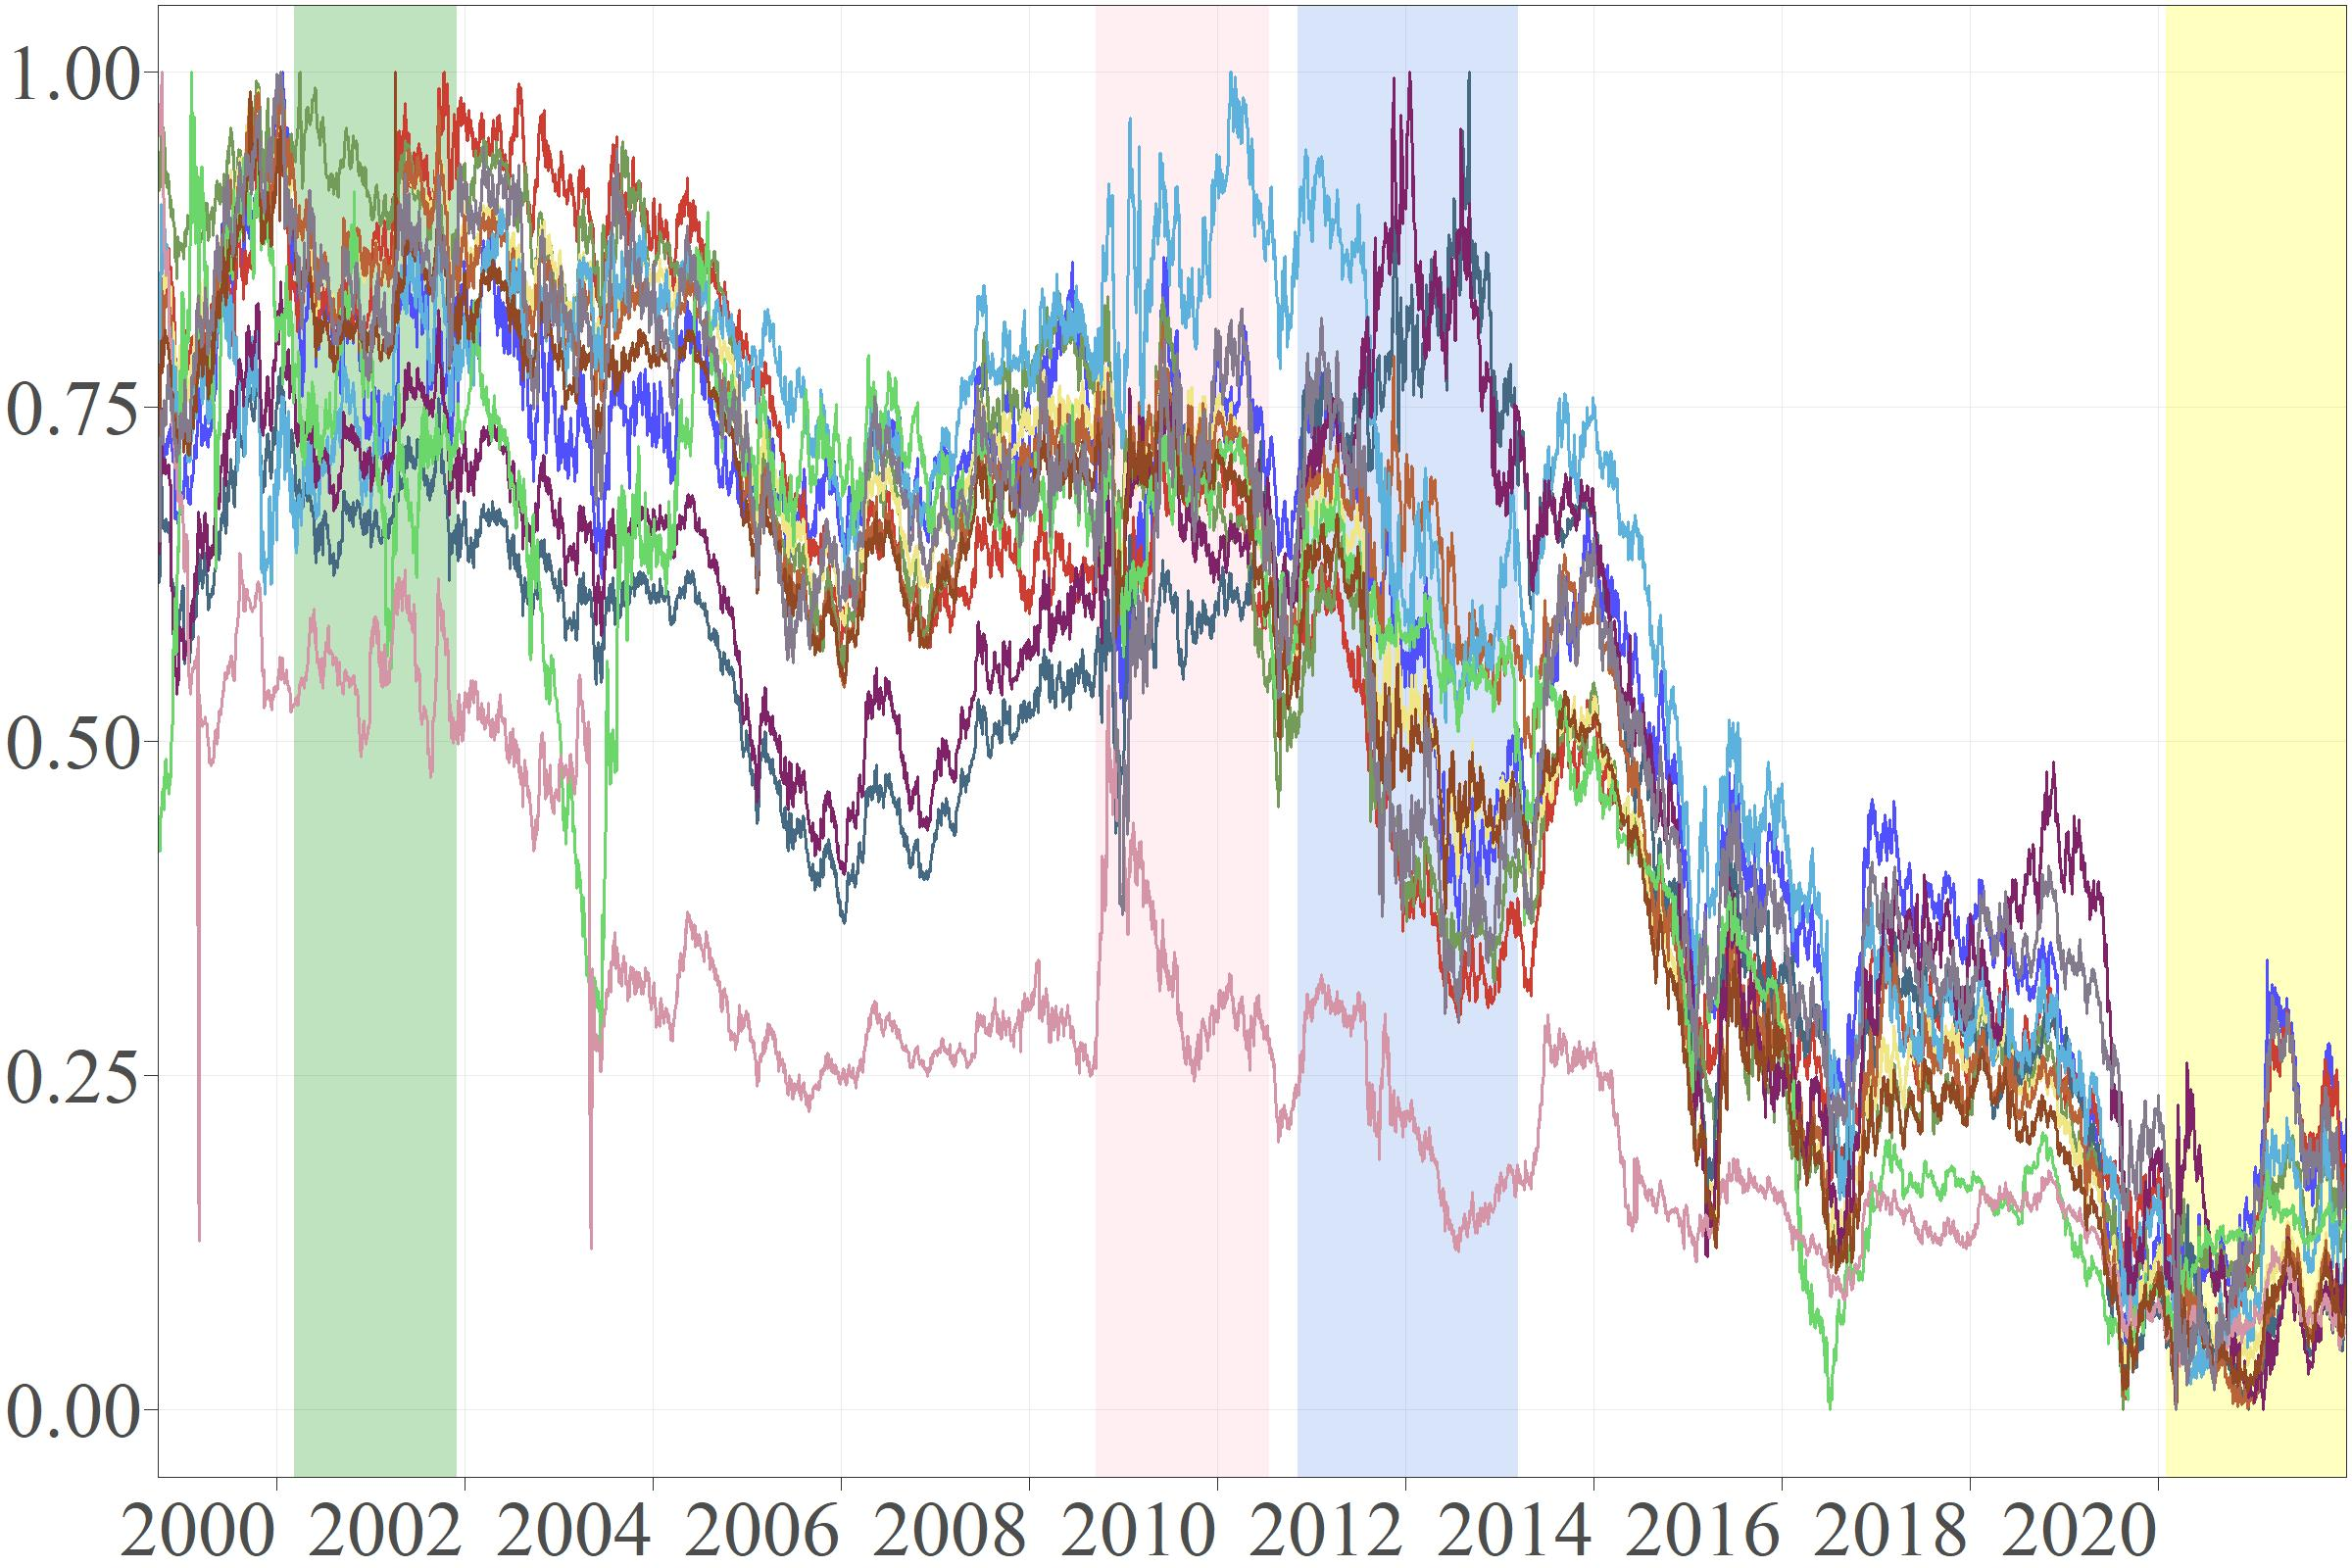
\includegraphics[width=\linewidth]{Level}
    \caption{\textbf{Level}}
\label{fig:levelTimeSeries}
  \end{subfigure}
  \hfill
  \begin{subfigure}[t]{.5\textwidth}
    \centering
    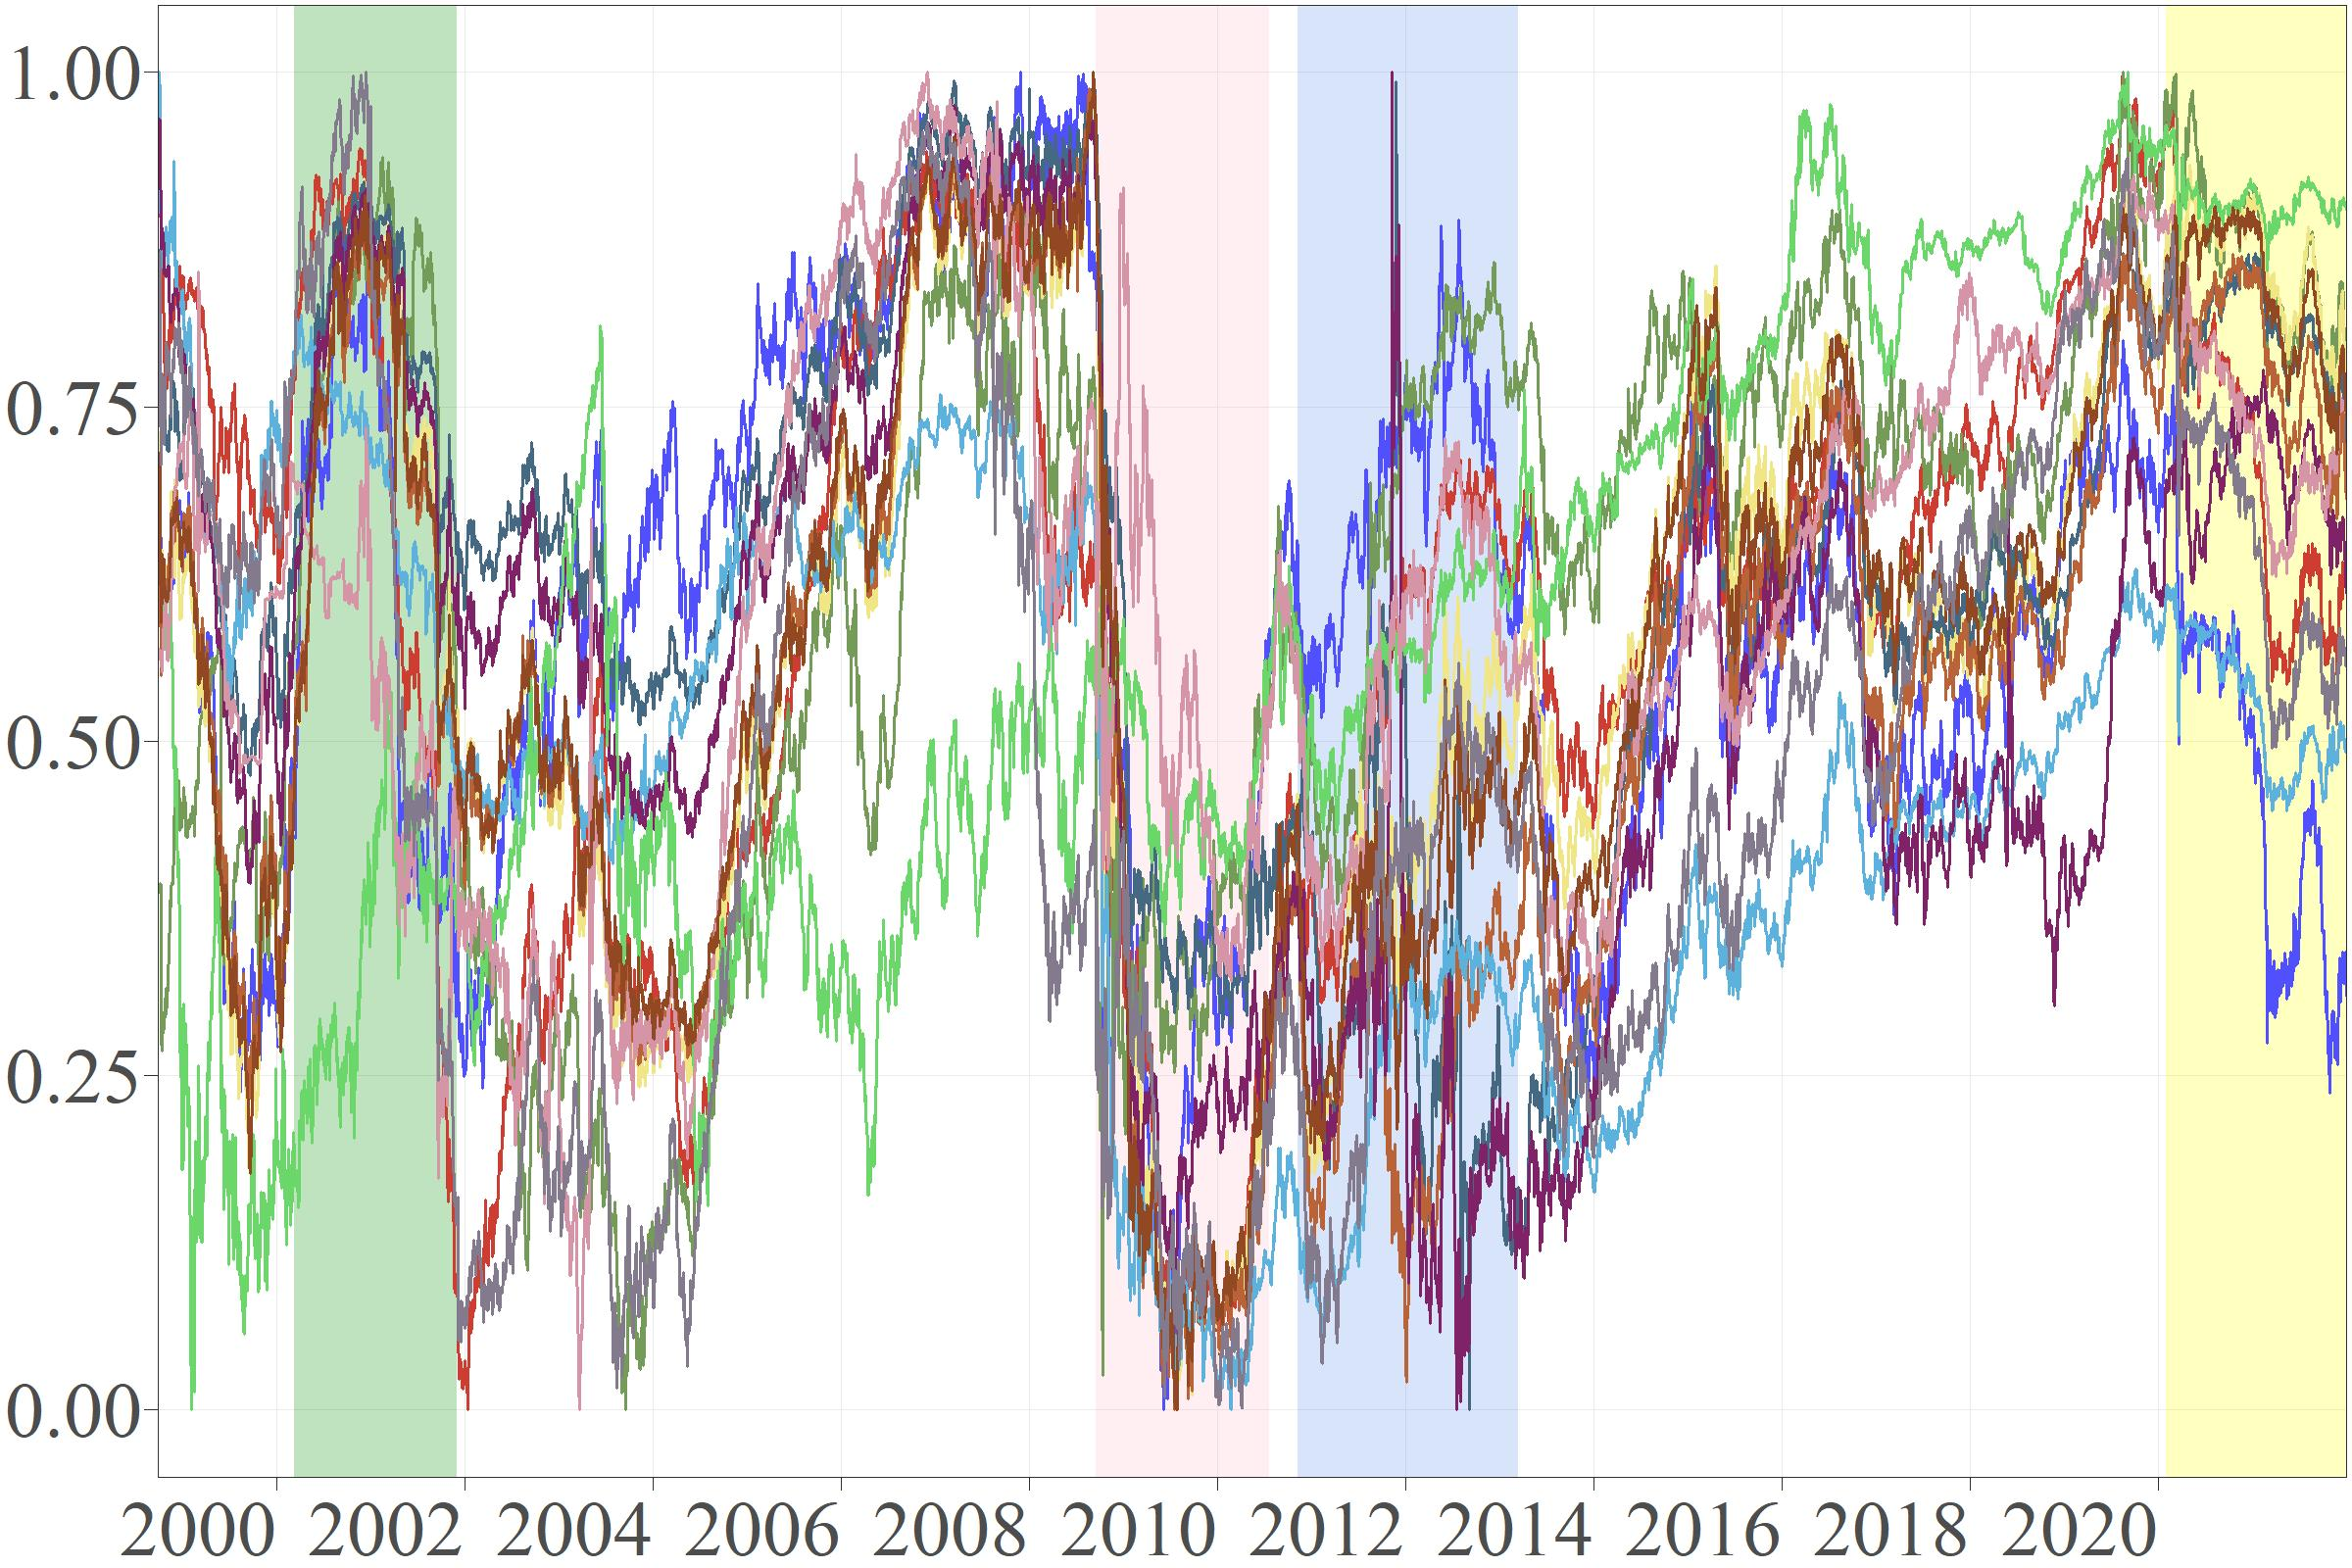
\includegraphics[width=\linewidth]{Slope}
    \caption{\textbf{Slope}}
\label{fig:slopeTimeSeries}
  \end{subfigure}

  \medskip

  \begin{subfigure}[t]{.5\textwidth}
    \centering
    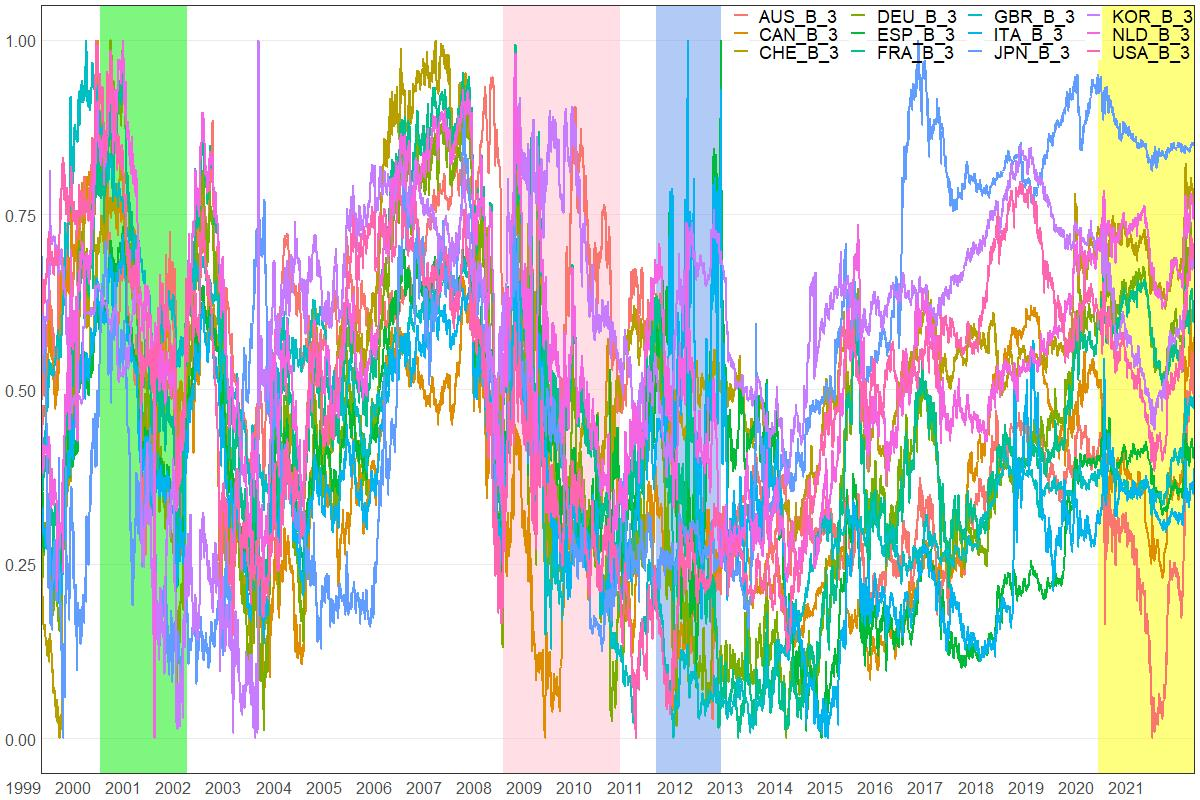
\includegraphics[width=\linewidth]{Curvature}
    \caption{\textbf{Curvature}}
\label{fig:curvatureRimeSeries}
  \end{subfigure}
  \hfill
  \begin{subfigure}[t]{.5\textwidth}
    \centering
    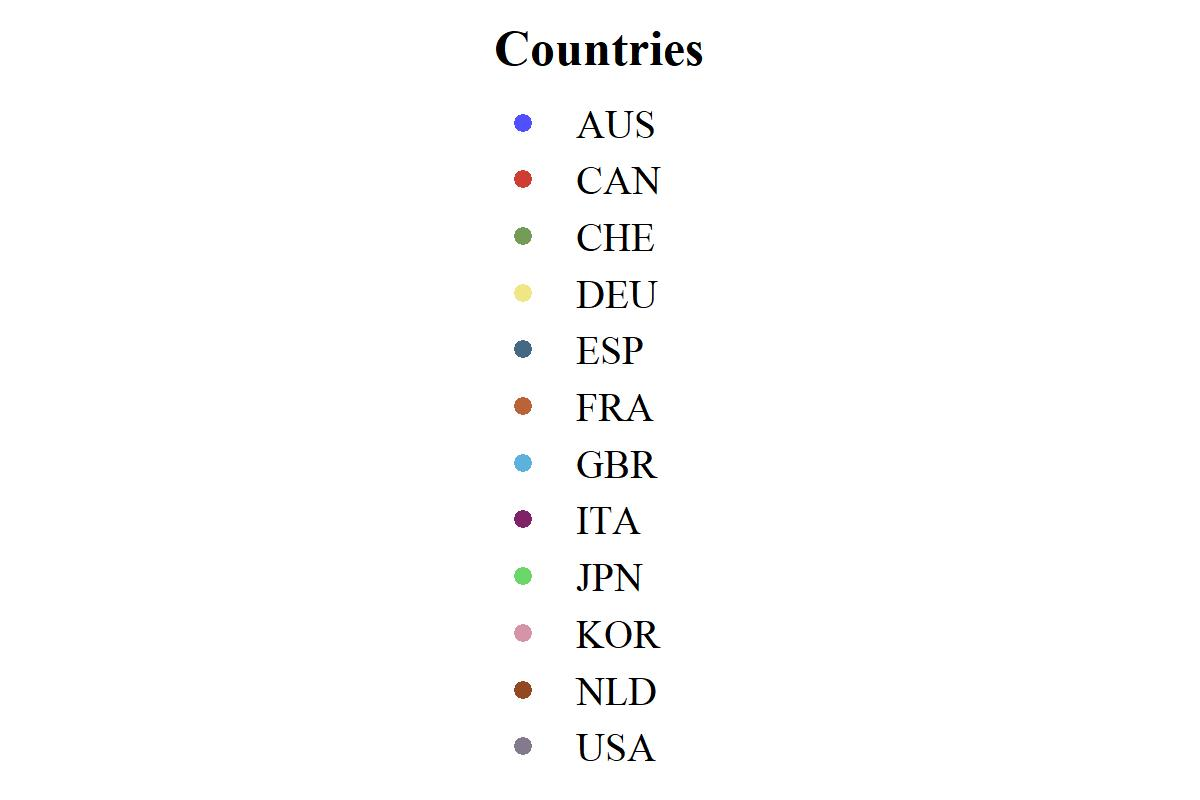
\includegraphics[width=\linewidth]{Legend}
  \end{subfigure}

\caption{Normlized factor time series}
\label{fig:factorTimeSeries}
\fnote{
Start of the dotcom bubble: NASDAQ Composite stock market index peaked at 5,048.62 (03/10/2000);

End of the dotcom bubble: Enron declared bankruptcy (12/02/2001);

\smallskip

Start of the subprime crisis: Bankruptcy of Lehman Brothers (09/15/2008);

End of subprime crisis: Dodd - Frank Act being enacted (07/21/2010);

\smallskip

Start of the European sovereign debt crisis: Ireland requests for IMF -  EU bailout (11/21/2010);

End of the European sovereign debt crisis: Ireland managed to regain complete lending access on financial markets (03/13/2013);

\smallskip

Start of Covid19 pandemic: WHO declared the coronavirus outbreak a global pandemic (01/20/2020). 
}

\end{figure}





%---------------------------------------------------------------------------------------------------------------------------------------------------------------------------

%\textcolor{red}{Es itt mondtad, hogy van egy eros faktorkomponens, arra egyelore nem nagyon tudok reagalni, azzal kapcsolatban mi lenne a tervunk?}

The descriptive statistics of the factors are represented in Table \ref{tab:descriptiveStatistics}. The average Level factors are positive in all cases, highest for South Korea and lowest for Japan. Average Slope refers to the typical increasing shape of the yield curves (negative values). The mean of Slope is negative for all countries meaning that longer maturities have higher values than shorter ones. In absolute terms Italy has the highest Slope, while Australia has the lowest. Potential positive values of Slope represent restrictive monetary politics. Average Curvature is always negative too, highest for Italy and lowest for Great Britain (in absolute terms).


%-----------------------------------------------------------------------------------Table1-----------------------------------------------------------------------------
\begin{table}[H]

\fontsize{10}{10}\selectfont
\centering % used for centering table
\begin{tabular}{l c c c c c c}% centered columns (4 columns)
\hline\hline   \\ [-1.5ex]               %inserts double horizontal lines
%Case & Method\#1 & Method\#2 & Method\#3 & test \\  [0.5ex]
Factor & Average & Std. dev. & Minimum & Maximum & Jarque-Bera t-stat.  & P value \\ [0.5ex] % inserts table %heading

\hline       \\ [-1.5ex]           % inserts single horizontal line


\textit{\textbf{Australia}}	&		&		&		&		&		&		\\
Level	&	4.87	&	1.50	&	1.06	&	7.71	&	540.29	&	0	\\
Slope	&	-1.11	&	0.99	&	-4.14	&	0.97	&	85.24	&	0	\\
Curvature	&	-2.15	&	1.90	&	-6.80	&	2.93	&	205.41	&	0	\\
\textit{\textbf{Canada}}	&		&		&		&		&		&		\\
Level	&	3.94	&	1.56	&	0.70	&	6.62	&	404.33	&	0	\\
Slope	&	-1.83	&	1.37	&	-5.35	&	0.58	&	364.08	&	0	\\
Curvature	&	-2.18	&	1.94	&	-6.27	&	4.83	&	400.29	&	0	\\
\textit{\textbf{Switzerland}}	&		&		&		&		&		&		\\
Level	&	2.19	&	1.56	&	-0.79	&	4.63	&	528.09	&	0	\\
Slope	&	-1.60	&	0.94	&	-4.10	&	-0.06	&	543.73	&	0	\\
Curvature	&	-2.71	&	1.49	&	-7.25	&	1.05	&	30.68	&	0	\\
\textit{\textbf{Germany}}	&		&		&		&		&		&		\\
Level	&	3.35	&	1.98	&	-0.55	&	6.56	&	542.63	&	0	\\
Slope	&	-1.84	&	1.11	&	-4.69	&	0.22	&	234.39	&	0	\\
Curvature	&	-3.51	&	1.73	&	-6.81	&	0.96	&	256.80	&	0	\\
\textit{\textbf{Spain}}	&		&		&		&		&		&		\\
Level	&	4.54	&	1.73	&	0.75	&	8.56	&	397.05	&	0	\\
Slope	&	-2.78	&	1.52	&	-7.35	&	-0.07	&	282.06	&	0	\\
Curvature	&	-4.01	&	2.09	&	-8.75	&	3.90	&	115.59	&	0	\\
\textit{\textbf{France}}	&		&		&		&		&		&		\\
Level	&	3.72	&	1.80	&	0.11	&	6.63	&	575.05	&	0	\\
Slope	&	-2.15	&	1.17	&	-4.85	&	0.16	&	241.96	&	0	\\
Curvature	&	-3.98	&	1.90	&	-8.08	&	0.57	&	47.29	&	0	\\
\textit{\textbf{Great Britain}}	&		&		&		&		&		&		\\
Level	&	3.69	&	1.37	&	0.47	&	5.77	&	764.03	&	0	\\
Slope	&	-1.39	&	1.73	&	-5.40	&	3.21	&	233.43	&	0	\\
Curvature	&	-1.82	&	3.58	&	-8.79	&	8.77	&	93.08	&	0	\\
\textit{\textbf{Italy}}	&		&		&		&		&		&		\\
Level	&	4.83	&	1.43	&	1.43	&	7.90	&	481.67	&	0	\\
Slope	&	-3.01	&	1.39	&	-6.36	&	-0.24	&	196.68	&	0	\\
Curvature	&	-4.19	&	1.96	&	-8.74	&	4.06	&	142.96	&	0	\\
\textit{\textbf{Japan}}	&		&		&		&		&		&		\\
Level	&	1.79	&	0.91	&	-0.03	&	3.57	&	599.64	&	0	\\
Slope	&	-1.43	&	0.75	&	-3.30	&	-0.09	&	318.65	&	0	\\
Curvature	&	-3.72	&	1.44	&	-6.54	&	-0.95	&	508.30	&	0	\\
\textit{\textbf{South Korea}}	&		&		&		&		&		&		\\
Level	&	6.13	&	2.49	&	1.88	&	17.23	&	842.90	&	0	\\
Slope	&	-3.00	&	1.58	&	-7.85	&	0.10	&	169.56	&	0	\\
Curvature	&	-4.17	&	3.00	&	-14.38	&	2.67	&	1961.09	&	0	\\
\textit{\textbf{The Netherlands}}	&		&		&		&		&		&		\\
Level	&	3.45	&	1.97	&	-0.36	&	7.01	&	539.12	&	0	\\
Slope	&	-1.95	&	1.14	&	-4.89	&	0.20	&	237.11	&	0	\\
Curvature	&	-3.30	&	1.57	&	-8.40	&	0.74	&	180.26	&	0	\\
\textit{\textbf{USA}}	&		&		&		&		&		&		\\
Level	&	4.39	&	1.45	&	0.96	&	6.98	&	383.47	&	0	\\
Slope	&	-2.44	&	1.72	&	-5.71	&	0.91	&	311.13	&	0	\\
Curvature	&	-3.61	&	2.68	&	-10.35	&	3.27	&	197.93	&	0	\\



\hline%inserts single line
\end{tabular}
\caption{Descriptive statistics of yield curve factors}% title of Table
\label{tab:descriptiveStatistics}% is used to refer this table in the text
\end{table}
%----------------------------------------------------------------------------------------------------------------------------------------------------

%------------------------------------------------ table2---------------------------------------------------------------------------------

\bigskip


Factor time sereies are tested with Jarque-Bera test for normality. Neither of them passes the acceptance criteria therefore the null-hypothesis for normaility is rejected. Furthermore ADF and KPSS unit-root tests for stationarity are applied. According to the ADF test, Level time series are stationary for Korea and USA, Slopre is stationary for Japan while Curvature is stationary for Australia and Italy on 99\% confidence level. According to the KPSS test, neither of the time series is stationary. The tests can be applied for first differenence of the remaining time series too. The first difference is stationary for all of the time series which is confirmed by both of the used tests. The unit-root test results are represented in Table \ref{tab:unitRootTest} in the Appendix.

Before differentiating, a pairwise Engle-Granger test is applied for determining cointegrations. Table \ref{tab:pairwiseEngleGranger} represents the ratio of the cointegrated time series aggregated by factors. Besides the diagonal, the Level - Curvature and the Slope - Curvature pairs both show a value more than 85\%. Since the time series are not stationary on the same order and the ratio of cointegrated time series is high, we consider the Toda-Yamamoto approach to be justified for analyzing connections.

%--------------------------------------------------------------------------------Table3 -------------------------------------------------------
\begin{table}[H]


\centering% centering table
\begin{tabular}{l  ccc}% creating eight columns
\hline\hline \\ [-1.5ex]                         %inserting double-line

	&	Level 	&	Slope	&	Curvature	\\
\hline \\ [-1.5ex]  
Level 		&81.8\%		&42.3\%	&87.3\% \\
Slope 		&16.2\%		&61.4\%	&91.5\% \\
Curvature 	&23.9\%		&62.0\%	&90.9\% \\



\hline            

\end{tabular}
% is used to refer this table in the text
\caption{Pairwise Engle-Granger test} %title of the table
\label{tab:pairwiseEngleGranger}% is used to refer this table in the text
\end{table}

    \begin{tablenotes}
      \small
     \item \centering \textit{Instead of the 36 x 36 matrix which we obtain from the pairwise Engle-Granger test, we highlight only the factor-wise aggregated values in this table.}
    \end{tablenotes}

%----------------------------------------------------------------------------------------------------------------------------------------------------


\section{Results}

\subsection{Static, full-sample interconnectedness}

We perform static and dynamic analysis of the factor interconnectedness resulted by the Toda-Yamamoto model. All of the available data points are used in the static method. Time series are differenciated once at maximum, and the optimal lag number is determined based on AIC. Figure \ref{fig:interrconnectednessInSubnetworks} shows the causailiy relationships on 1\% sigificance level. Level factors are red, while Slopes are blue and the Curvatures are showed in green. The arrow between two factors shows the direction of the causality and its color represent the factor which it is started from.

From the three subsystems, the Slope network is the most dense. 35.61\% of the potential relationships is significant. It is followed by Curvature (27.27\%), then Level (25.76\%). Considering cross connections, 11.0\% of the possible edges going out from Slope factors is significant. This ratio is 10.53\% for Level, and Curvature is the least interconnected factor in these terms, only 8.33\% of the outgoing edges is significant. Alltogether 258 significant cross connections can be defined which is 29.86\% of the total possible edges 864.

Even tought the short end of the yield curve (represented by the Slope) is less correlated than the long end (represented by the Level), synchronicity in the business cycles across the countries leads to some synchronicity in the monetary policy as well. Our results reinforces the statement of \cite{kumar2011dynamics} who claims that the slope factor is correlated within different countries.

%--------------------------------------------------------------------------------Fig3 -------------------------------------------------------
\begin{figure}[H]

  \begin{subfigure}[t]{.5\textwidth}
    \centering
    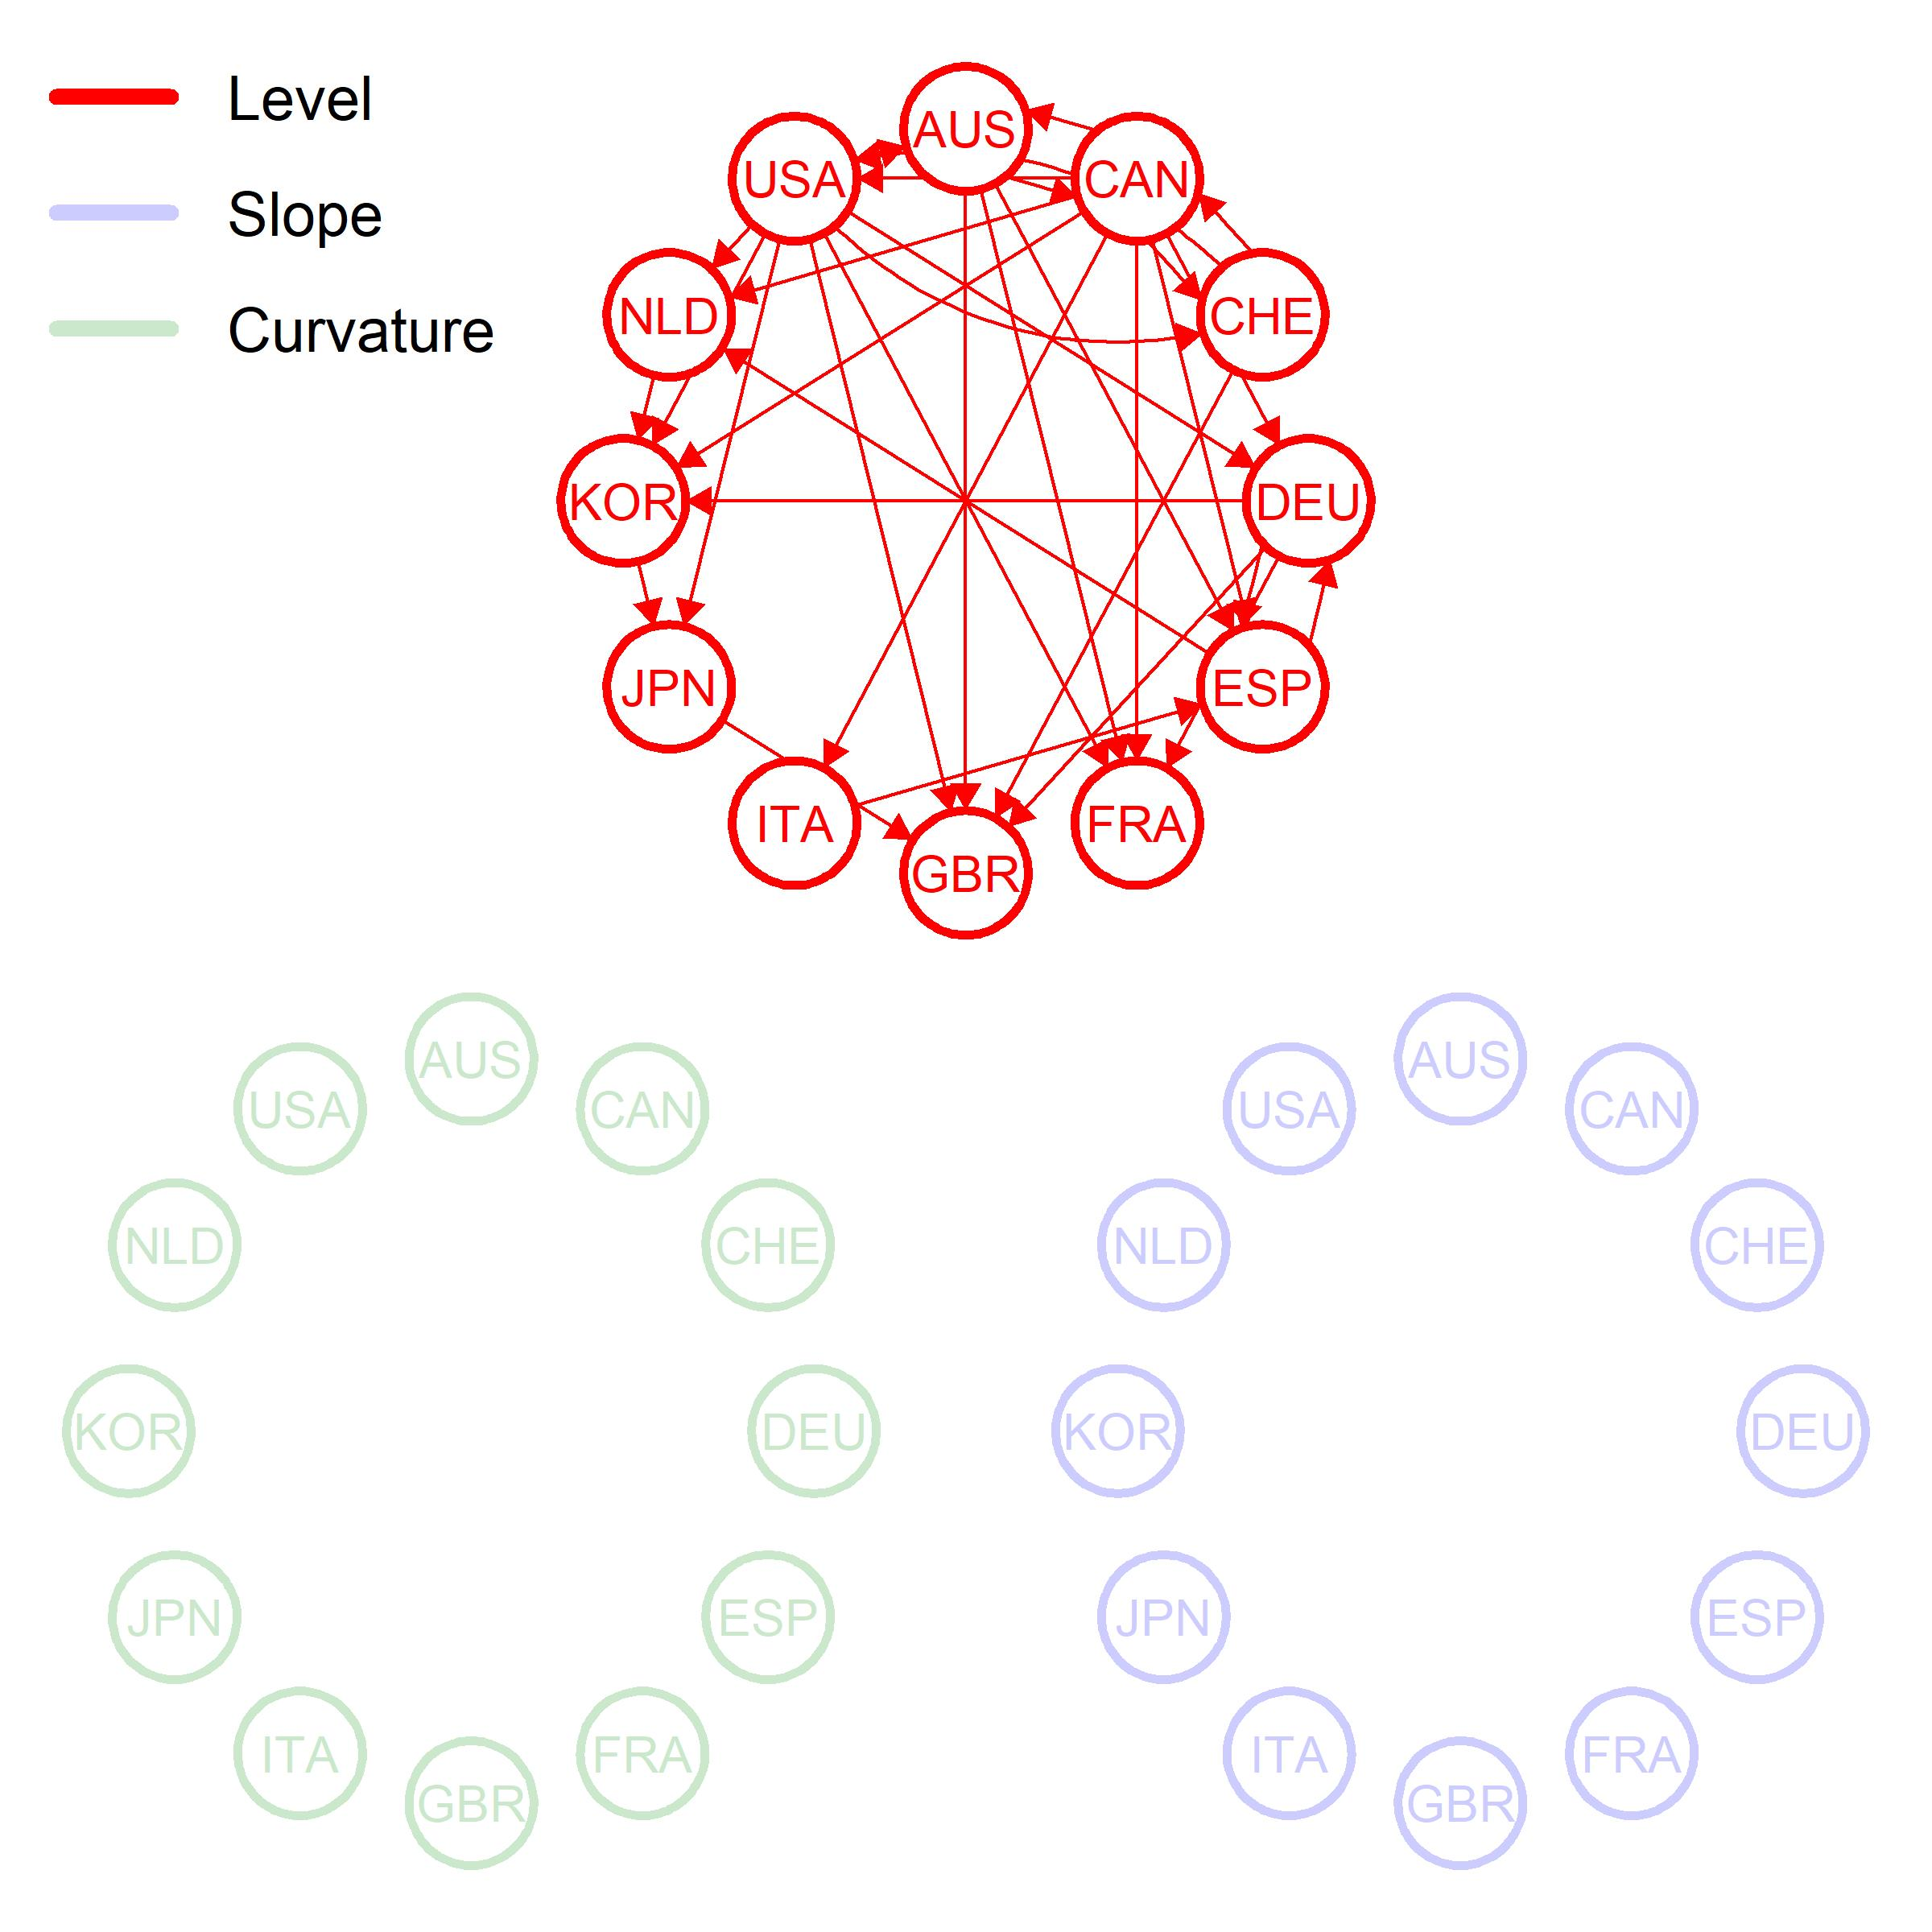
\includegraphics[width=\linewidth]{levelOnly_1998-09-30_2021-12-29_TY_fix}
    \caption{\textbf{Level subnetwork}}
\label{fig:levelSubnetwork}
  \end{subfigure}
  \hfill
  \begin{subfigure}[t]{.5\textwidth}
    \centering
    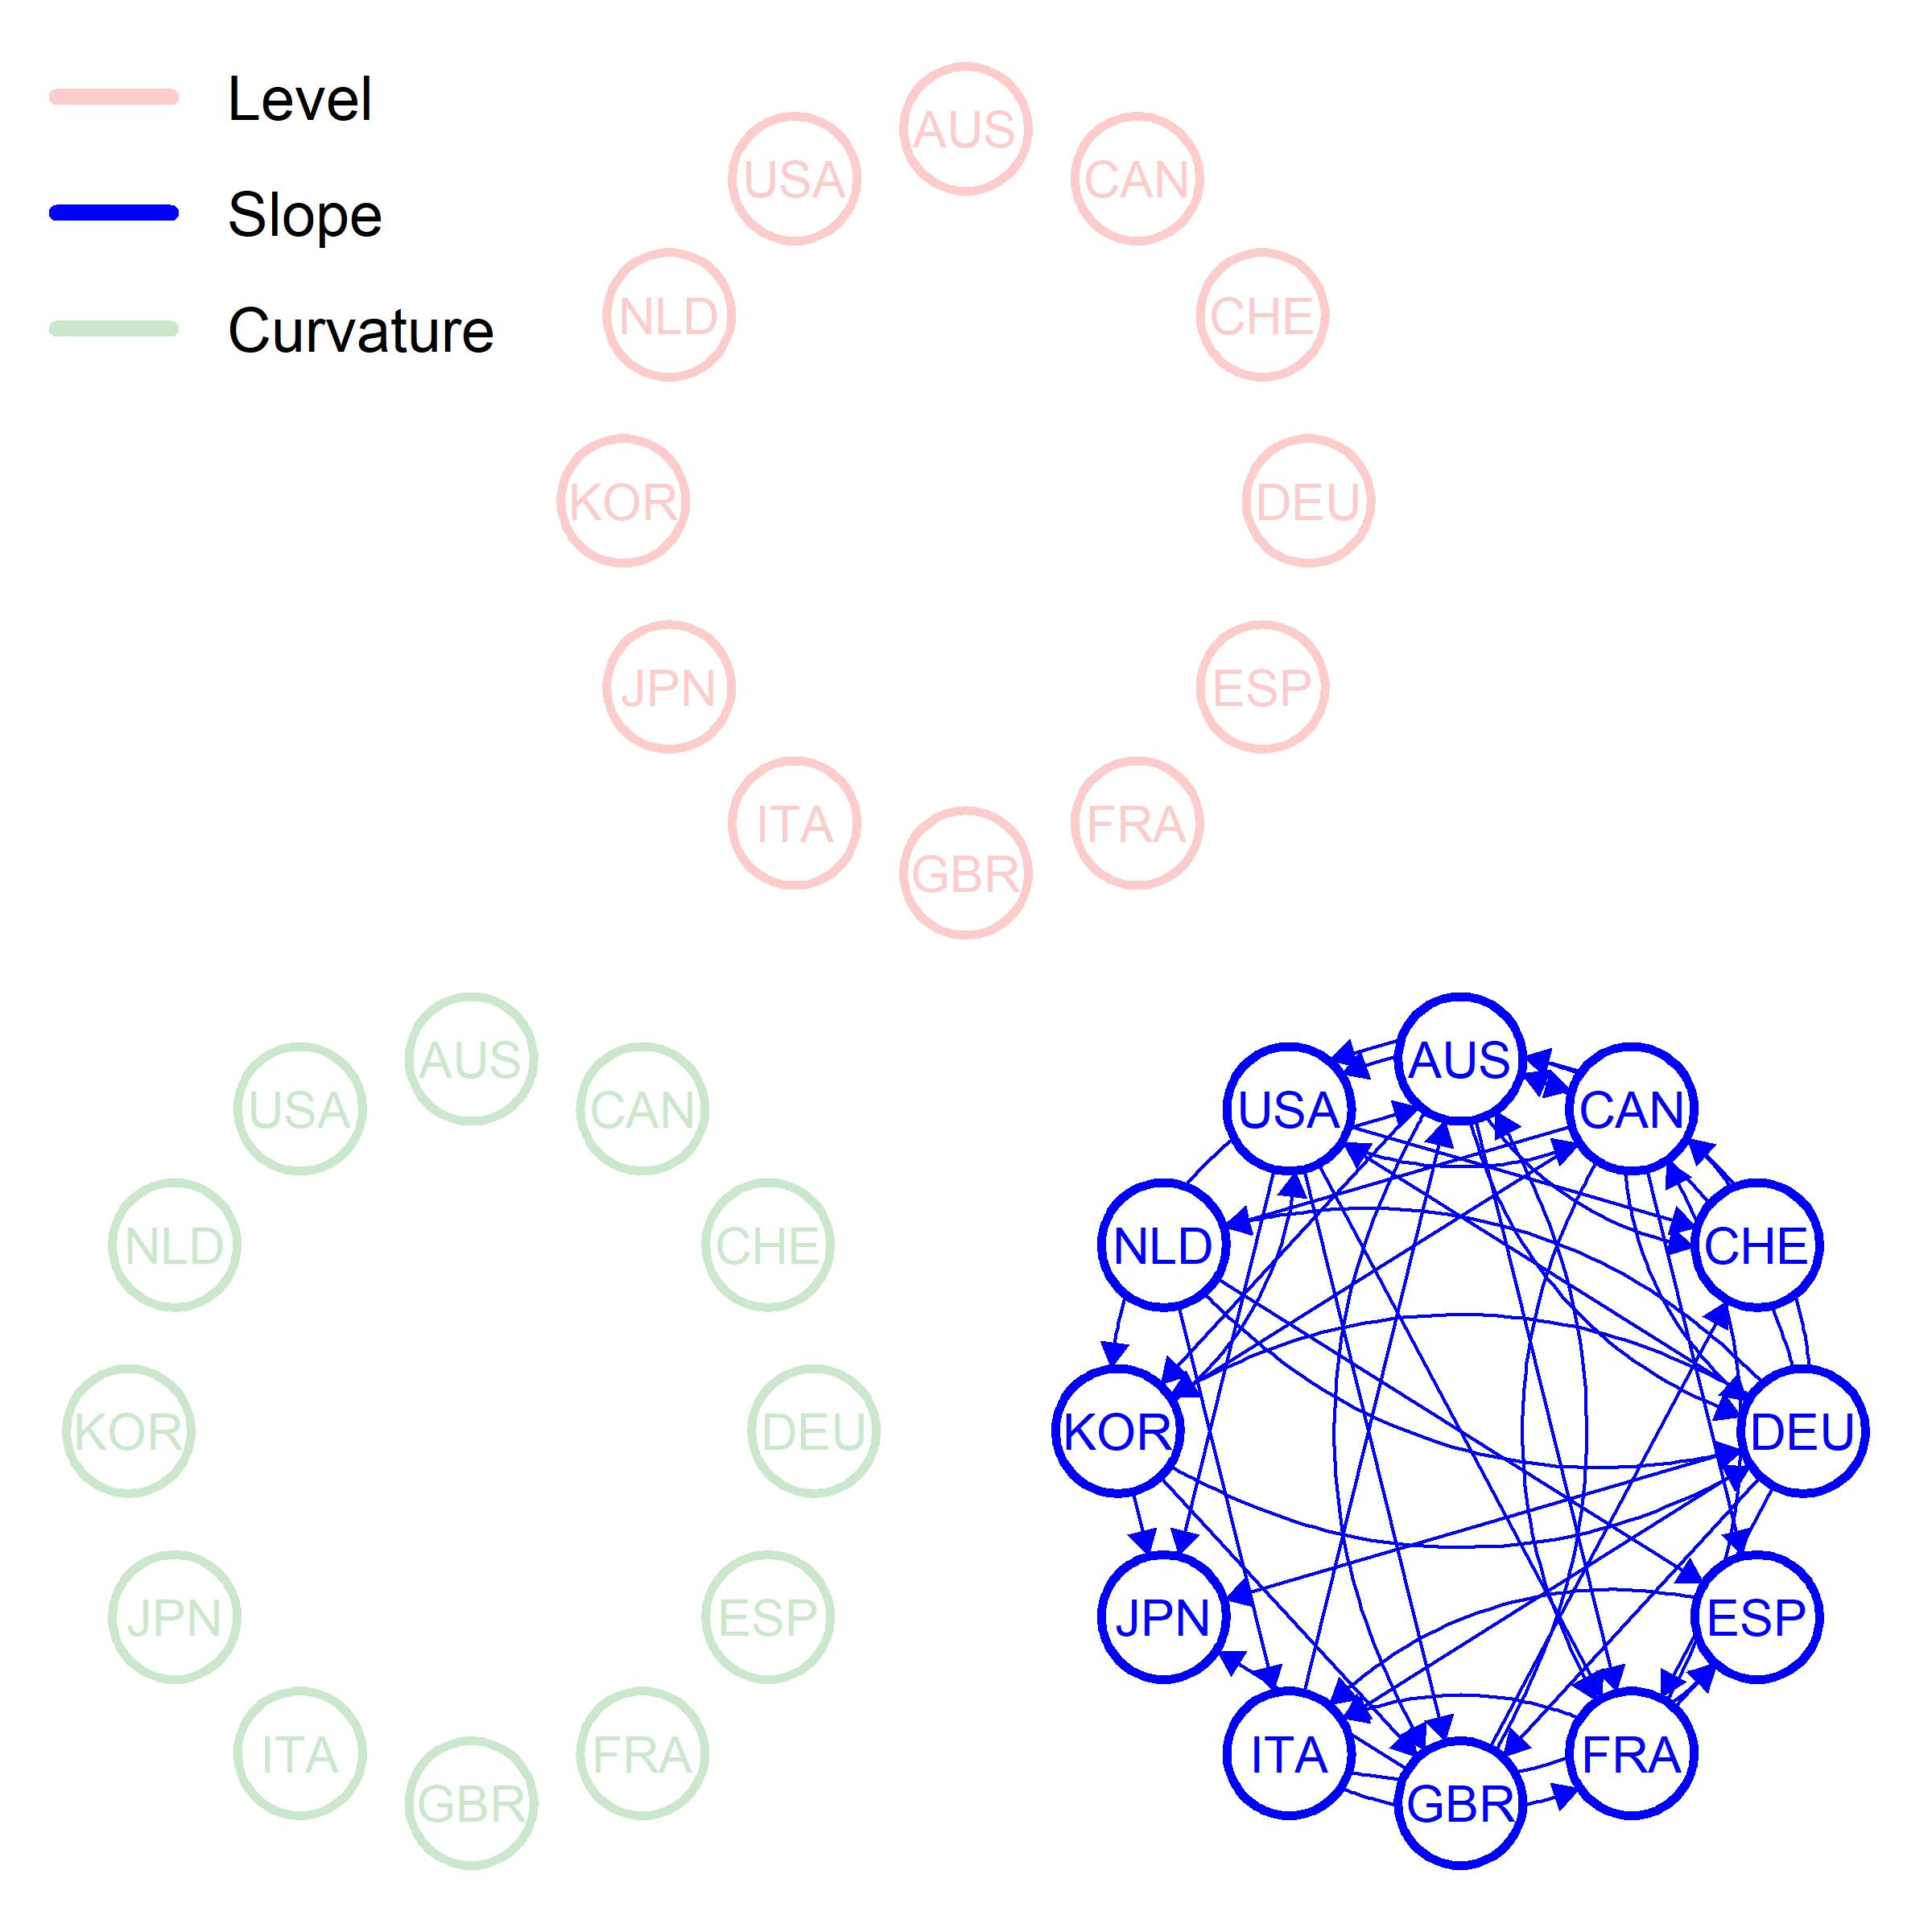
\includegraphics[width=\linewidth]{slopeOnly_1998-09-30_2021-12-29_TY_fix}
    \caption{\textbf{Slope subnetwork}}
\label{fig:slopeSubnetwork}
  \end{subfigure}

  \medskip

  \begin{subfigure}[t]{.5\textwidth}
    \centering
    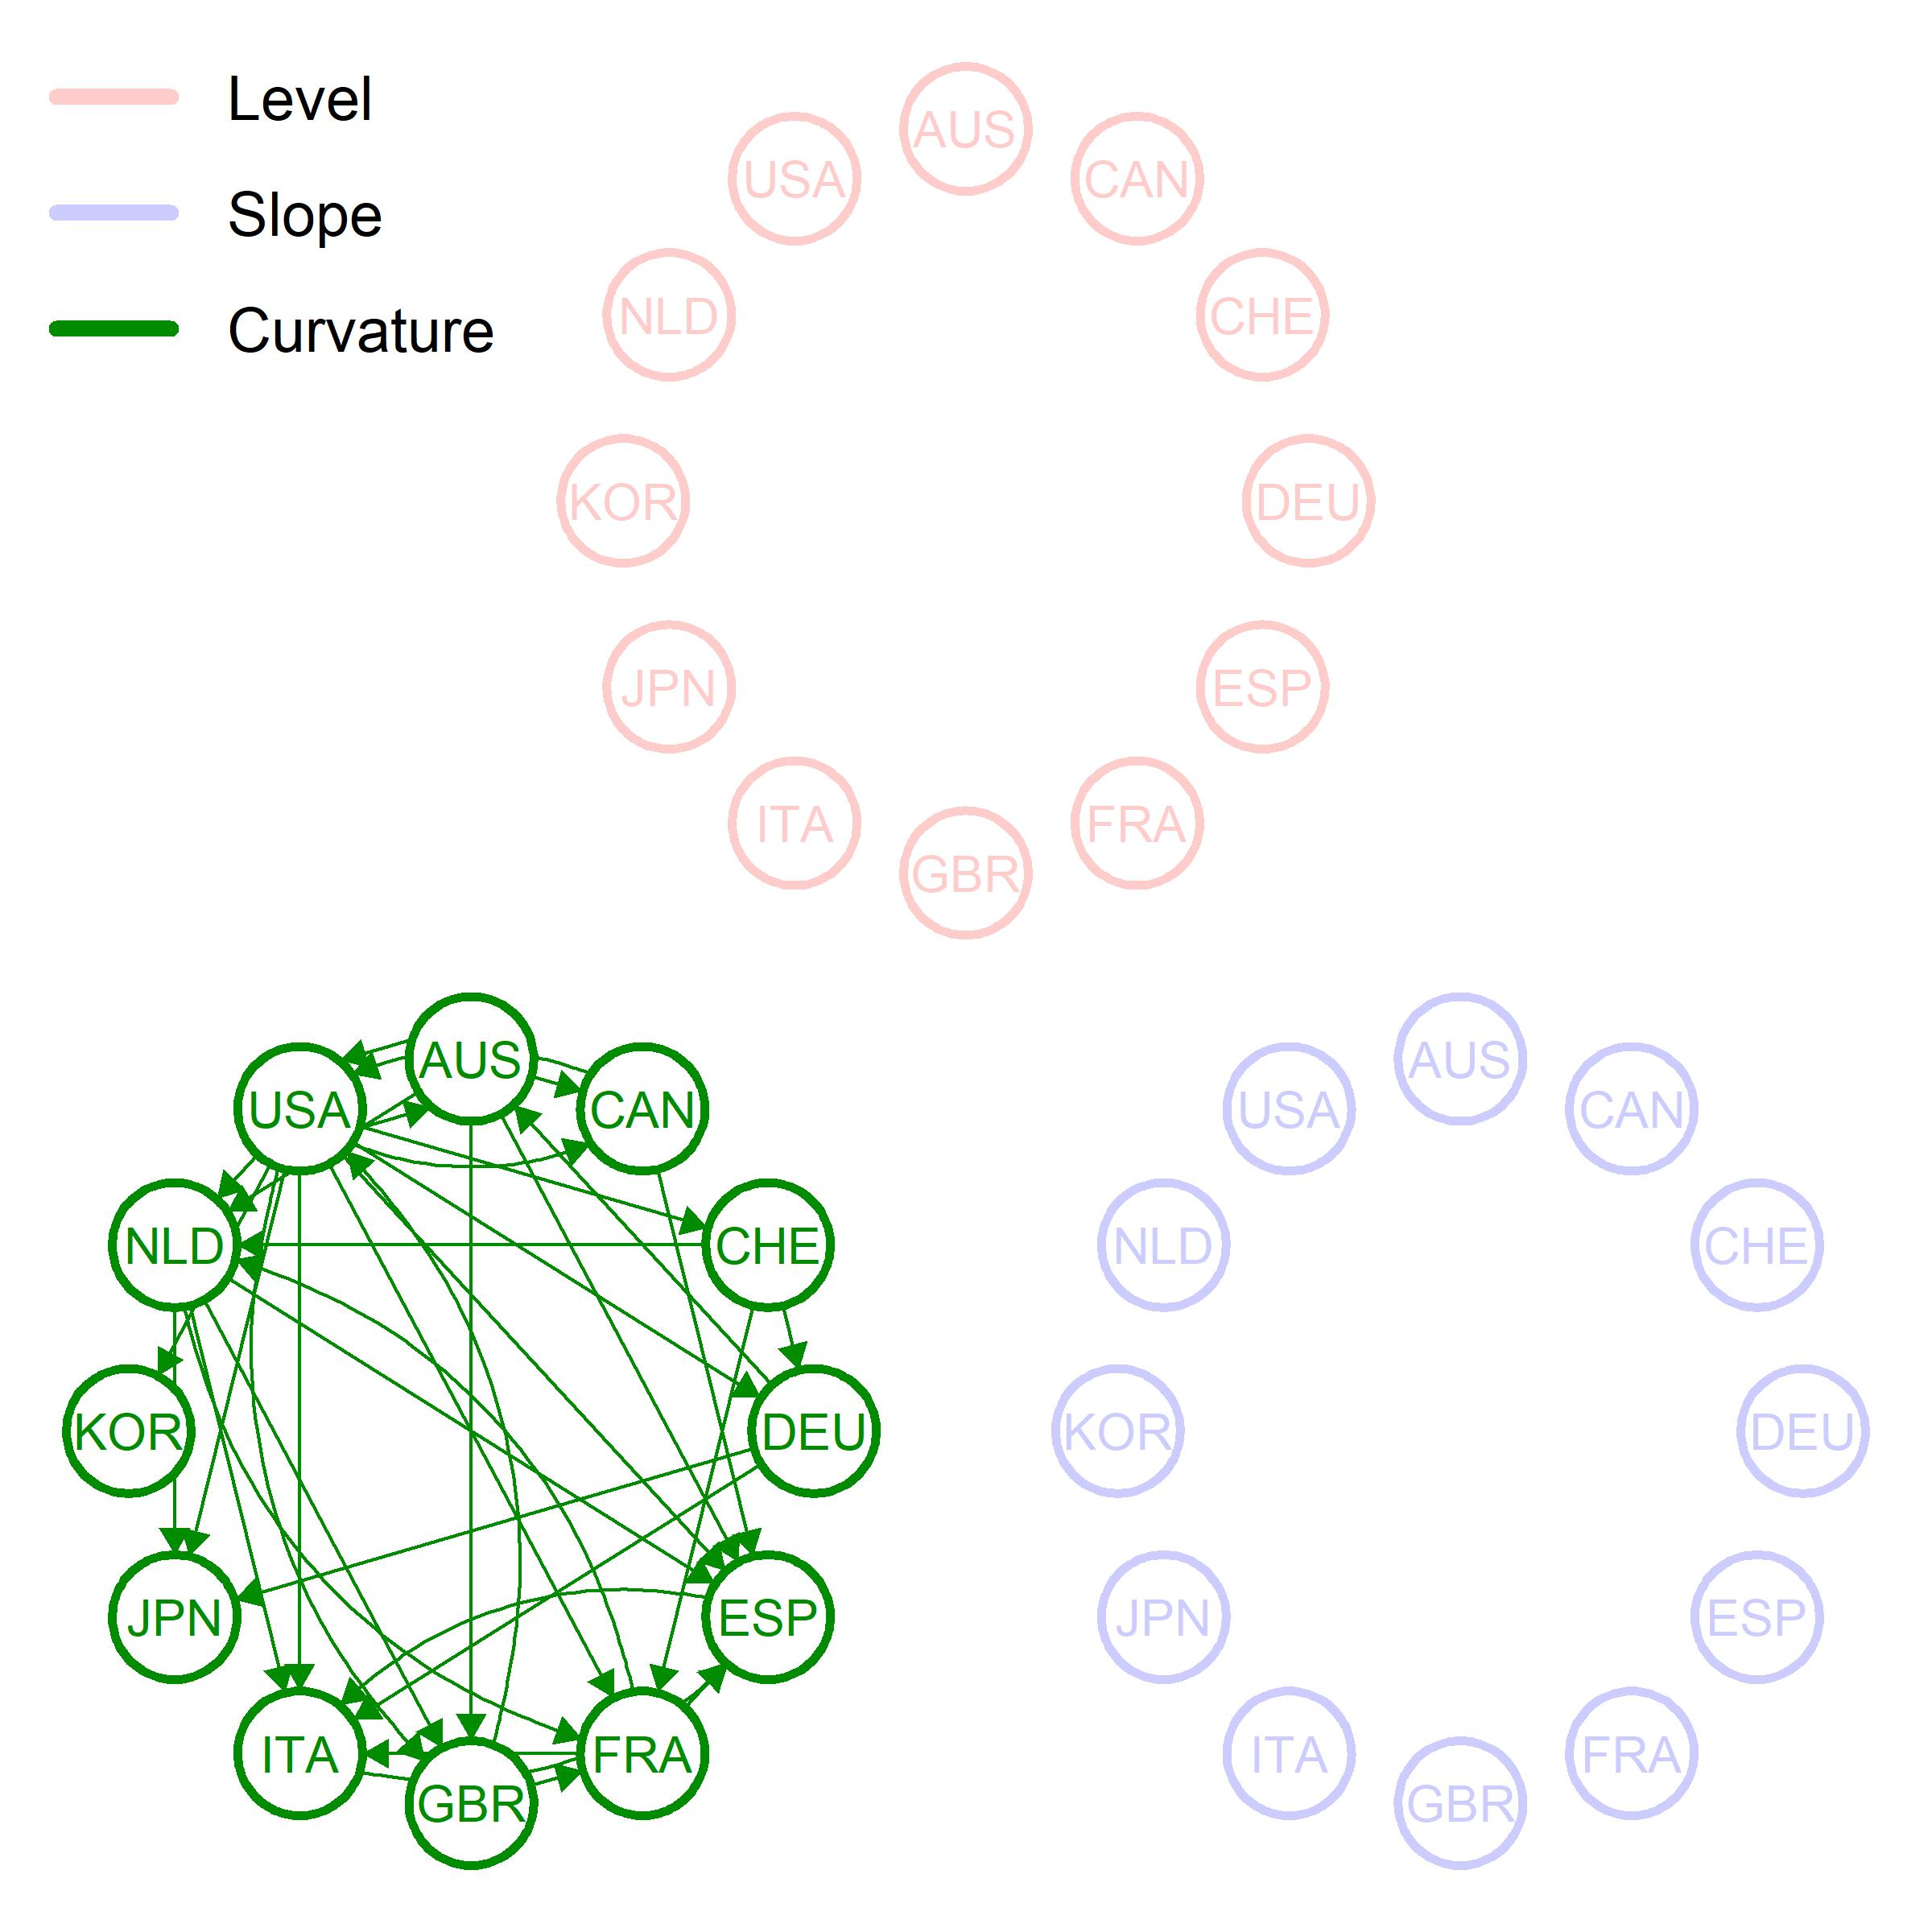
\includegraphics[width=\linewidth]{curvatureOnly_1998-09-30_2021-12-29_TY_fix}
    \caption{\textbf{Curvature subnetwork}}
\label{fig:curvatureSubnetwork}
  \end{subfigure}
  \hfill
  \begin{subfigure}[t]{.5\textwidth}
    \centering
    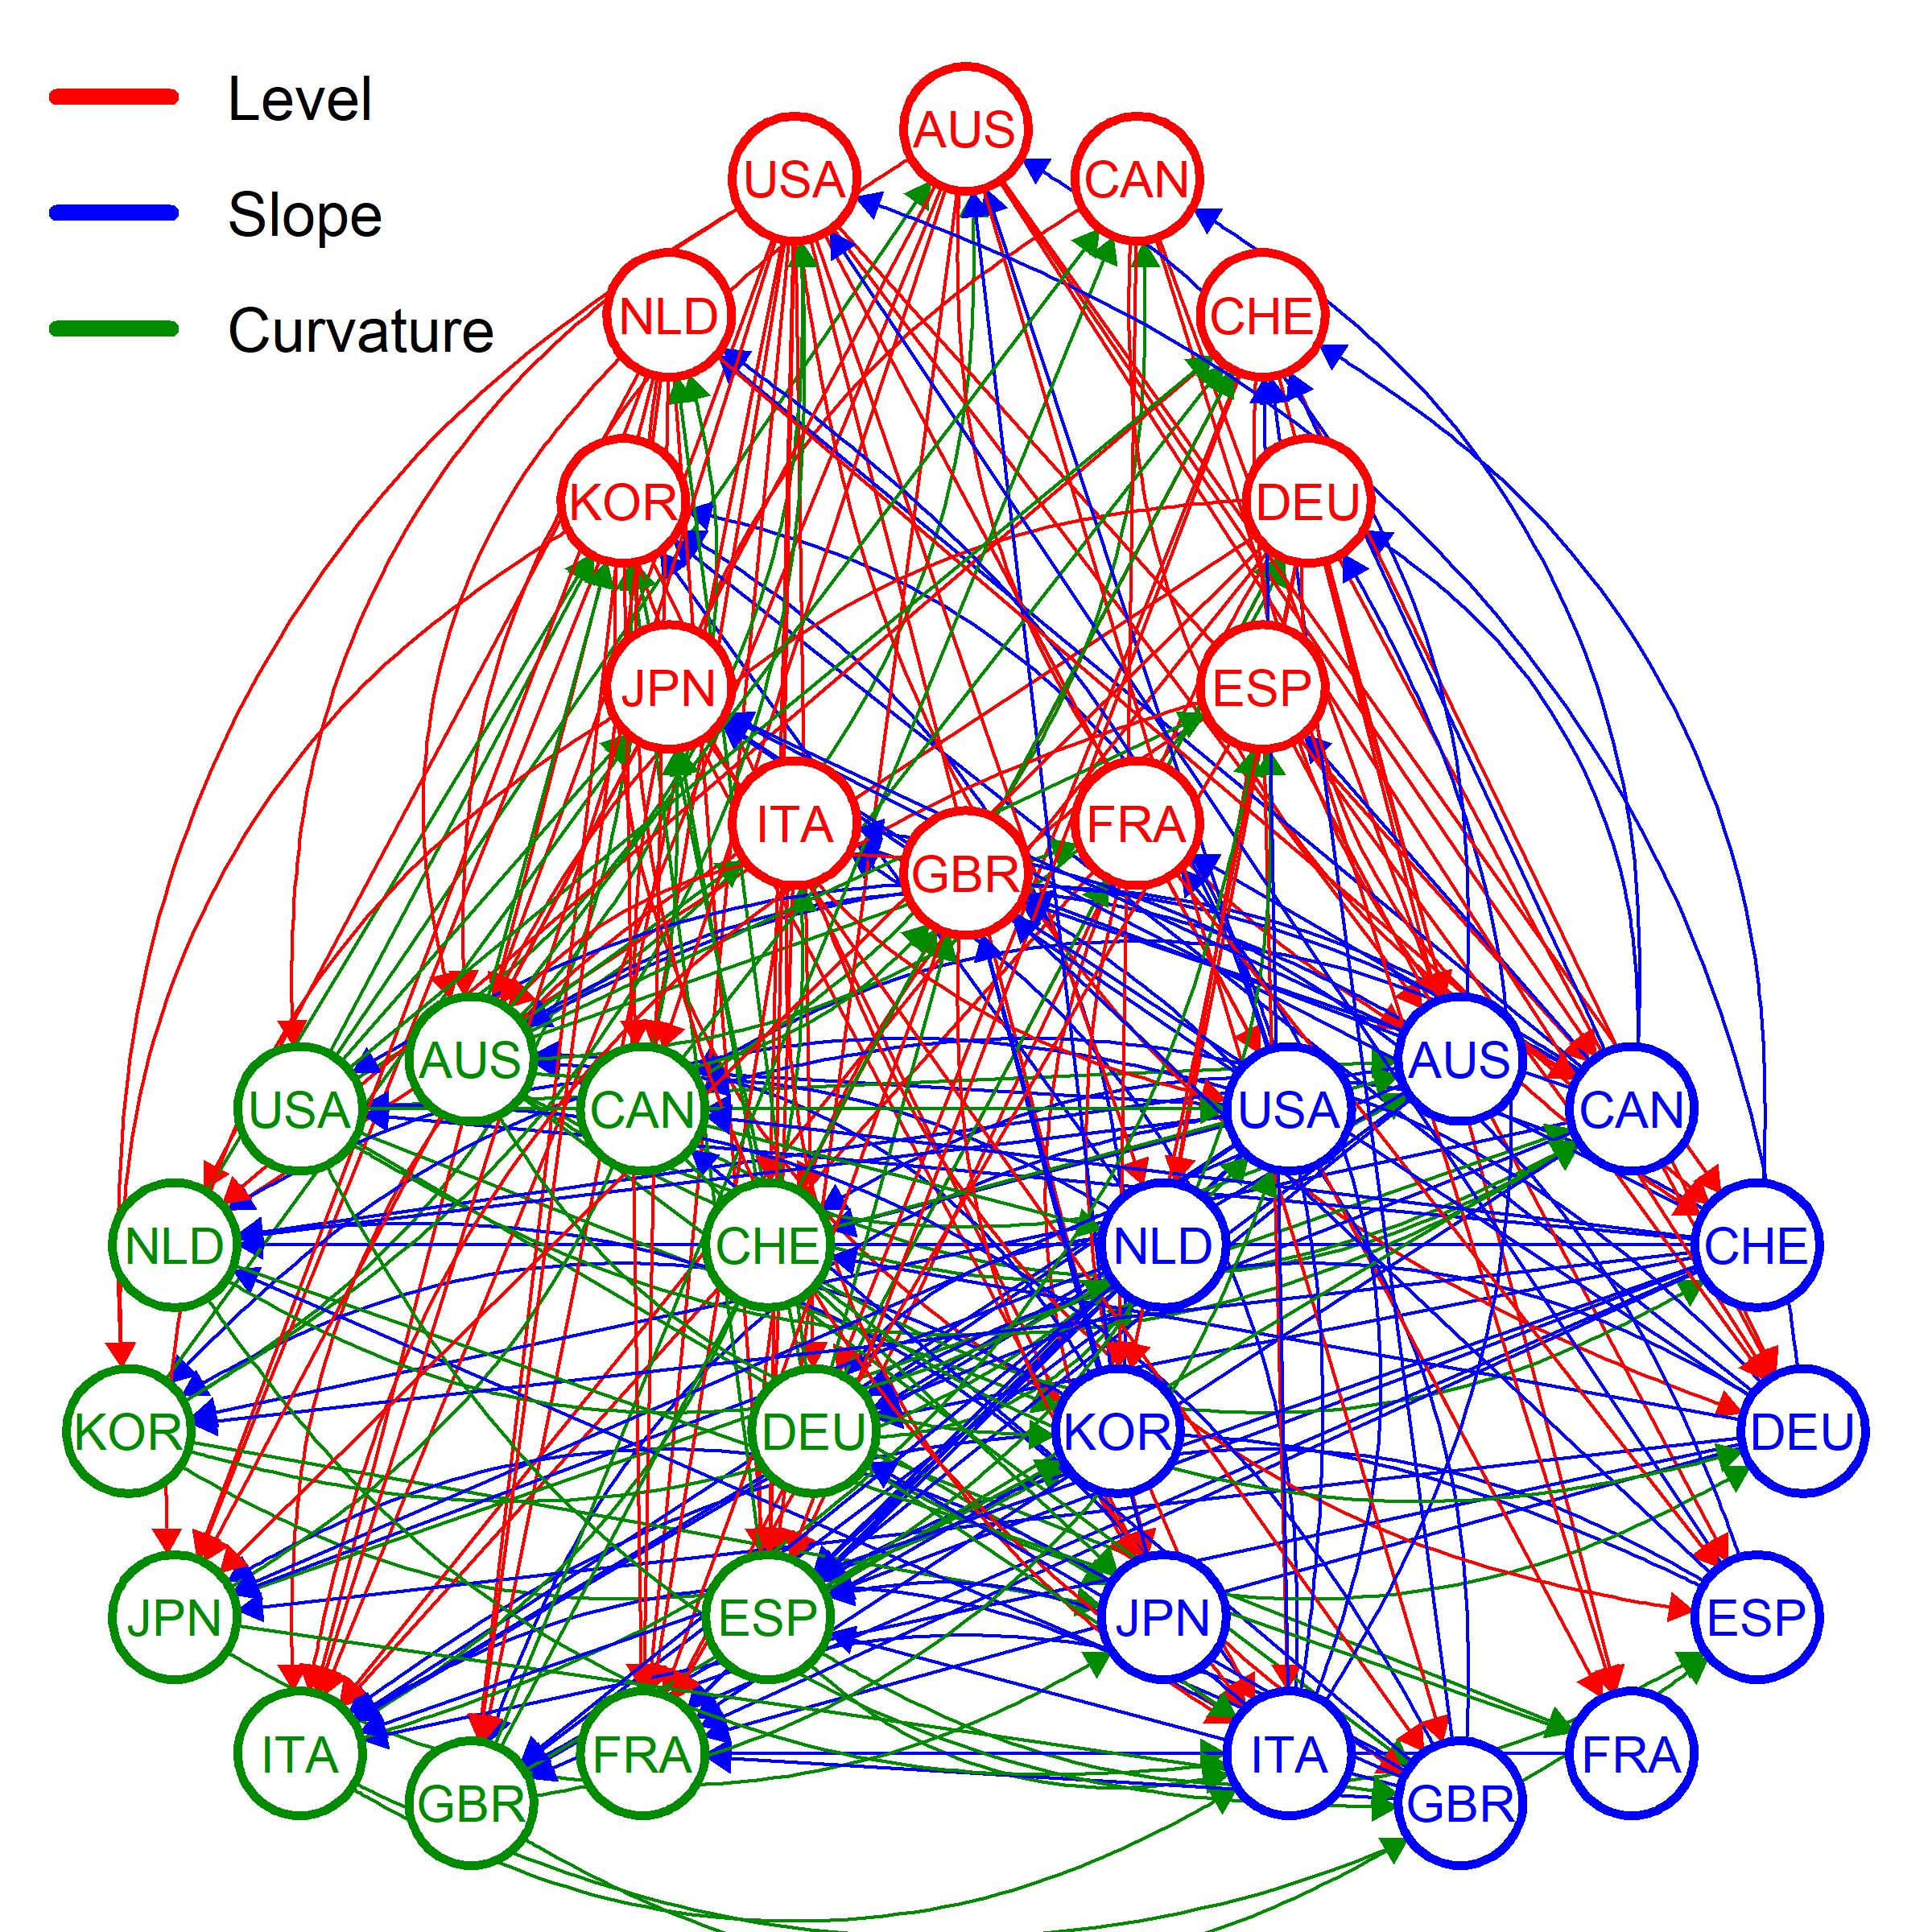
\includegraphics[width=\linewidth]{innerEmpty_1998-09-30_2021-12-29_TY_fix}
    \caption{\textbf{Cross connections}}
\label{fig:crossConnections}
  \end{subfigure}
  \caption{Interconnectedness in subnetworks}
\label{fig:interrconnectednessInSubnetworks}

\fnote{
In case of Level factors, 34 edges are significant form the total possible 132 which is 25.76\%;

In case of Slope factors, 47 edges are significant form the total possible 132 which is 35.61\%;

In case of Curvature factors, 36 edges are significant form the total possible 132 which is 27.27\%;

In case of cross connections, 258 edges are significant form the total possible 864 which is 29.46\%;

In case of total connections, 375 edges are significant form the total possible 1260 which is 29.76\%;

}




\end{figure}

%----------------------------------------------------------------------------------------------------------------------------------------------------

\bigskip

%A 4. táblázat (a) része tartalmazza a rendszerben definiált élek számát. A táblázat sorai a kapcsolatok eredetét mutatják, az oszlopok pedig a nyilak végpontjaira utalnak. 1\%-os szignifikancia szinten, a gráfnak 318 éle van, ami az összes lehetséges élnek a 25.24\%-a. A 4. táblázat (b) része tartalmazza az alrendszerek között definiált élek arányát, az abban a viszonyrendszerben értelmezett maximális kapcsolatok számához képest. Ezek alapján elmondható, hogy a Szint és Görbület közötti okság a legsűrűbb, 36.1\%, ezt követi a Meredekség és Görbület közötti összekö-töttség, 31.94\%-kal, a harmadik helyen pedig a Szint alhálózat alatt értelmezett nyilak aránya áll, 31.06\%-kal. A kapcsolati mátrix nem szimmetrikus a főátlóra, a Görbület faktorokból, összesítve kevesebb nyíl irányul mind az alhálózaton belülre, mind kívülre.

On the aggregate level we can say that Curvature factor has the most incoming edges, while Slope has he most outgoing ones. Level has the least incoming edges while it is second in the list of outgoing edges. In this sense, curvature can be said to be the least interconnected factor which is in line with the findings of \cite{dewachter2006macro} and \cite{diebold2006forecasting}
%--------------------------------------------------------------------------Table4--------------------------------------------------------------------------


\begin{table}[H]

\fontsize{9}{9}\selectfont
\centering
\begin{subtable}[t]{0.35\textwidth}
\centering
\begin{tabular}{l  ccc  r}% creating eight columns
\hline\hline \\ [-1.5ex]                         %inserting double-line

	&	Level 	&	Slope	&	Curvature	& Sum  \\ 
\hline \\ [-1.5ex]  
Level	&	34	&	43	&	48	&	 125	\\
Slope	&	33	&	47	&	62	&	142	\\
Curvature	&	34	&	38	&	36	&	108	\\
\hline \\ [-1.5ex]  
Sum	&	101	&	128	&	146	&	375	\\


\hline            
\end{tabular}
\caption{\textbf{Number of edges, grouped by factors}}
\label{tab:numberOfEdges}
%\label{table:nonlin}% is used to refer this table in the text
\end{subtable}
\hspace{\fill}
\begin{subtable}[t]{0.5\textwidth}
\centering
\begin{tabular}{l  ccc  r}% creating eight columns
\hline\hline \\ [-1.5ex]                         %inserting double-line



	&	Level	&	Slope	&	Curvature	&	Sum.	\\
\hline \\ [-1.5ex] 
Level	&	25.8\%	&	29.9\%	&	33.3\%	&	29.8\%	\\
Slope	&	22.9\%	&	35.6\%	&	43.1\%	&	33.8\%	\\
Curvature	&23.6\%	&	26.4\%	&	27.3\%	&	25.7\%	\\
\hline \\ [-1.5ex]  
Sum.	&	24.0\%	&	30.5\%	&	34.8\%	&	29.8\%	\\
\hline  
\end{tabular}
\caption{\textbf{Distribution of edges, grouped by factors}}
\label{tab:distributionOfEdges}
%\label{table:nonlin}% is used to refer this table in the text
\end{subtable}
\caption{The number and distibution of the sygnificant edges defined in the system} %title of the table
\label{tab:numberAndDistributionOfEdges}

\fnote{
 In the diagonal we divide the edge count by 132 \textit{($12\times(12-1)$)}, since this is  the maximum definable edge number in a sole subnetwork. 

\smallskip

Between two subnetwork this number is 144 \textit{($12\times12$)}, we scale the upper and lower triangulars by this. 

\smallskip

The values in the summarized row and colum are divided by 420 (132+144+144).

\smallskip

The total definable edges in the whole subnetwork is 1260 \textit{($420\times3$)}, we divide 375 by this.}

\end{table}
%----------------------------------------------------------------------------------------------------------------------------------------------------

\subsubsection{Top nodes}

Table \ref{tab:mostEdges} represents the factors with the most edges. The first quarter of the list stands for the summarized relationships, then the following columns represent the nodes having the most incoming and outgoing edges separatedly. In total, Slope factor of  Canada has the highest count of edges, which is 32. Fom this, there are 19 outgoing and 13 incoming arrows. Net (outgoing-incoming) edges can be a more reliable measure when one wants to identify the dominant participans of the system. All three factors of the USA leads the list of net edges. This can be interpreted as the USA having a high affecting power on the values of the factors of the remaining participants and in the meanwhile this country is less affected by the others. The Fed (and the US yieldcurve) being in a key role is determined by \cite{brusa2020one} and hereby we reinforce their conclusion. Figure \ref{fig:usaFactors} shows the causality relationships of the USA Level, Slope and Curvature factors. In the list of outgoing edges the USA is also dominant. 
The most causality effect is arriving towards the Spanish Curvature followed by the Italian Curvature and French Curvature factors.

%--------------------------------------------------------------------------Table5--------------------------------------------------------------------------
\begin{table}[h]

\fontsize{10}{10}\selectfont
\setlength{\tabcolsep}{10pt}
\centering% centering table
\begin{tabular}{l  lcc  lc lc  lc}% creating eight columns

\hline\hline \\ [-1.5ex]                         %inserting double-line


\multicolumn{4}{c}{Top 5 Sum}			&	\multicolumn{2}{c}{Top 5 Incoming}&	\multicolumn{2}{c}{Top 5 Outgoing}&	\multicolumn{2}{c}{Top 5 Net}	\\	
\hline \\ [-1.5ex]    
Node	&	Total 	&	In	&	Out	&	Node	&	In	&	Node	&	Out	&	Node	&	Net	\\
\hline \\ [-1.5ex]    
CAN\_S 	&	32	&	13	&	19	&	ESP\_C	&	20	&	USA\_L	&	25	&	USA\_L	&	19	\\
USA\_L	&	31	&	6	&	25	&	ITA\_C	&	19	&	USA\_C	&	22	&	USA\_C	&	15	\\
AUS\_C	&	30	&	12	&	18	&	FRA\_C	&	18	&	USA\_S	&	20	&	USA\_S	&	11	\\
AUS\_S	&	29	&	13	&	16	&	KOR\_L	&	14	&	CAN\_S	&	19	&	DEU\_L	&	9	\\
DEU\_S	&	29	&	11	&	18	&	ITA\_S	&	14	&	DEU\_S	&	18	&	CAN\_L	&	8	\\

\hline            
\end{tabular}


\caption{Factors having most edges} %title of the table
\label{tab:mostEdges}

\end{table}


%----------------------------------------------------------------------------------------------------------------------------------------------------



%--------------------------------------------------------------------------Fig4--------------------------------------------------------------------------
\begin{figure}[H]

  \begin{subfigure}[t]{.5\textwidth}
    \centering
    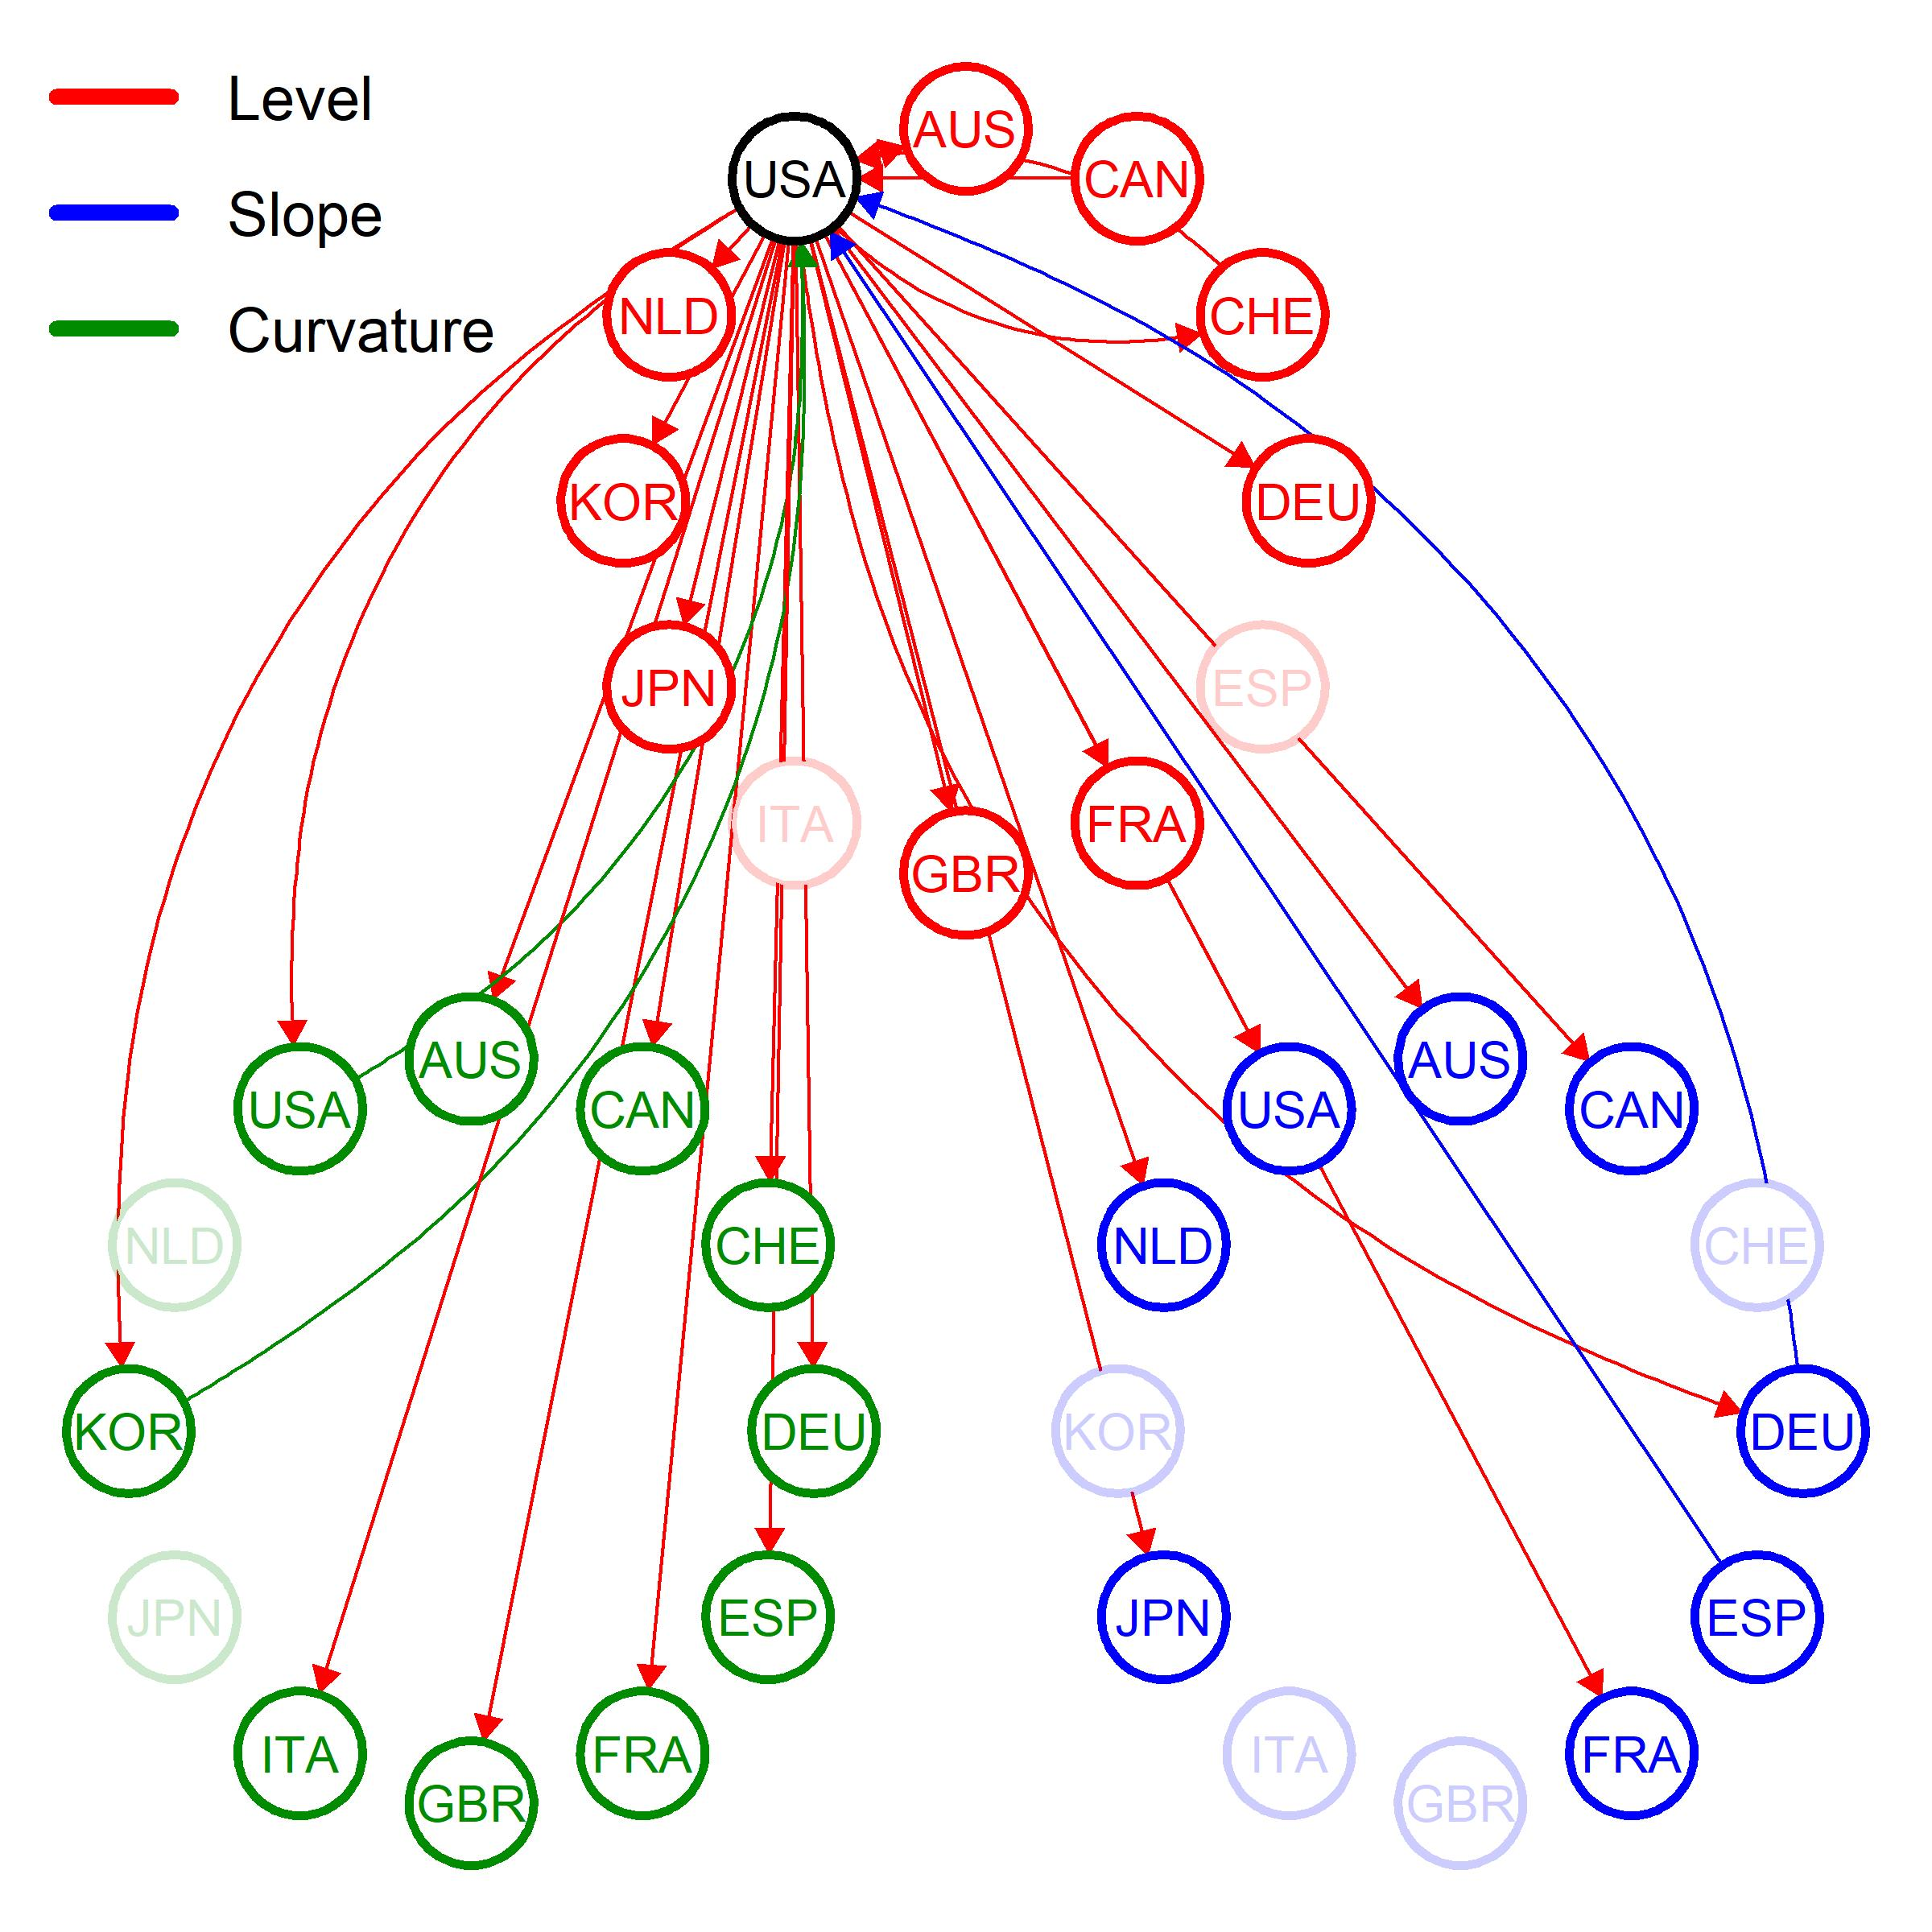
\includegraphics[width=\linewidth]{node_USA_B_1_1998-09-30_2021-12-29_TY_fix}
    \caption{\textbf{USA Level}}
  \end{subfigure}
  \hfill
  \begin{subfigure}[t]{.5\textwidth}
    \centering
    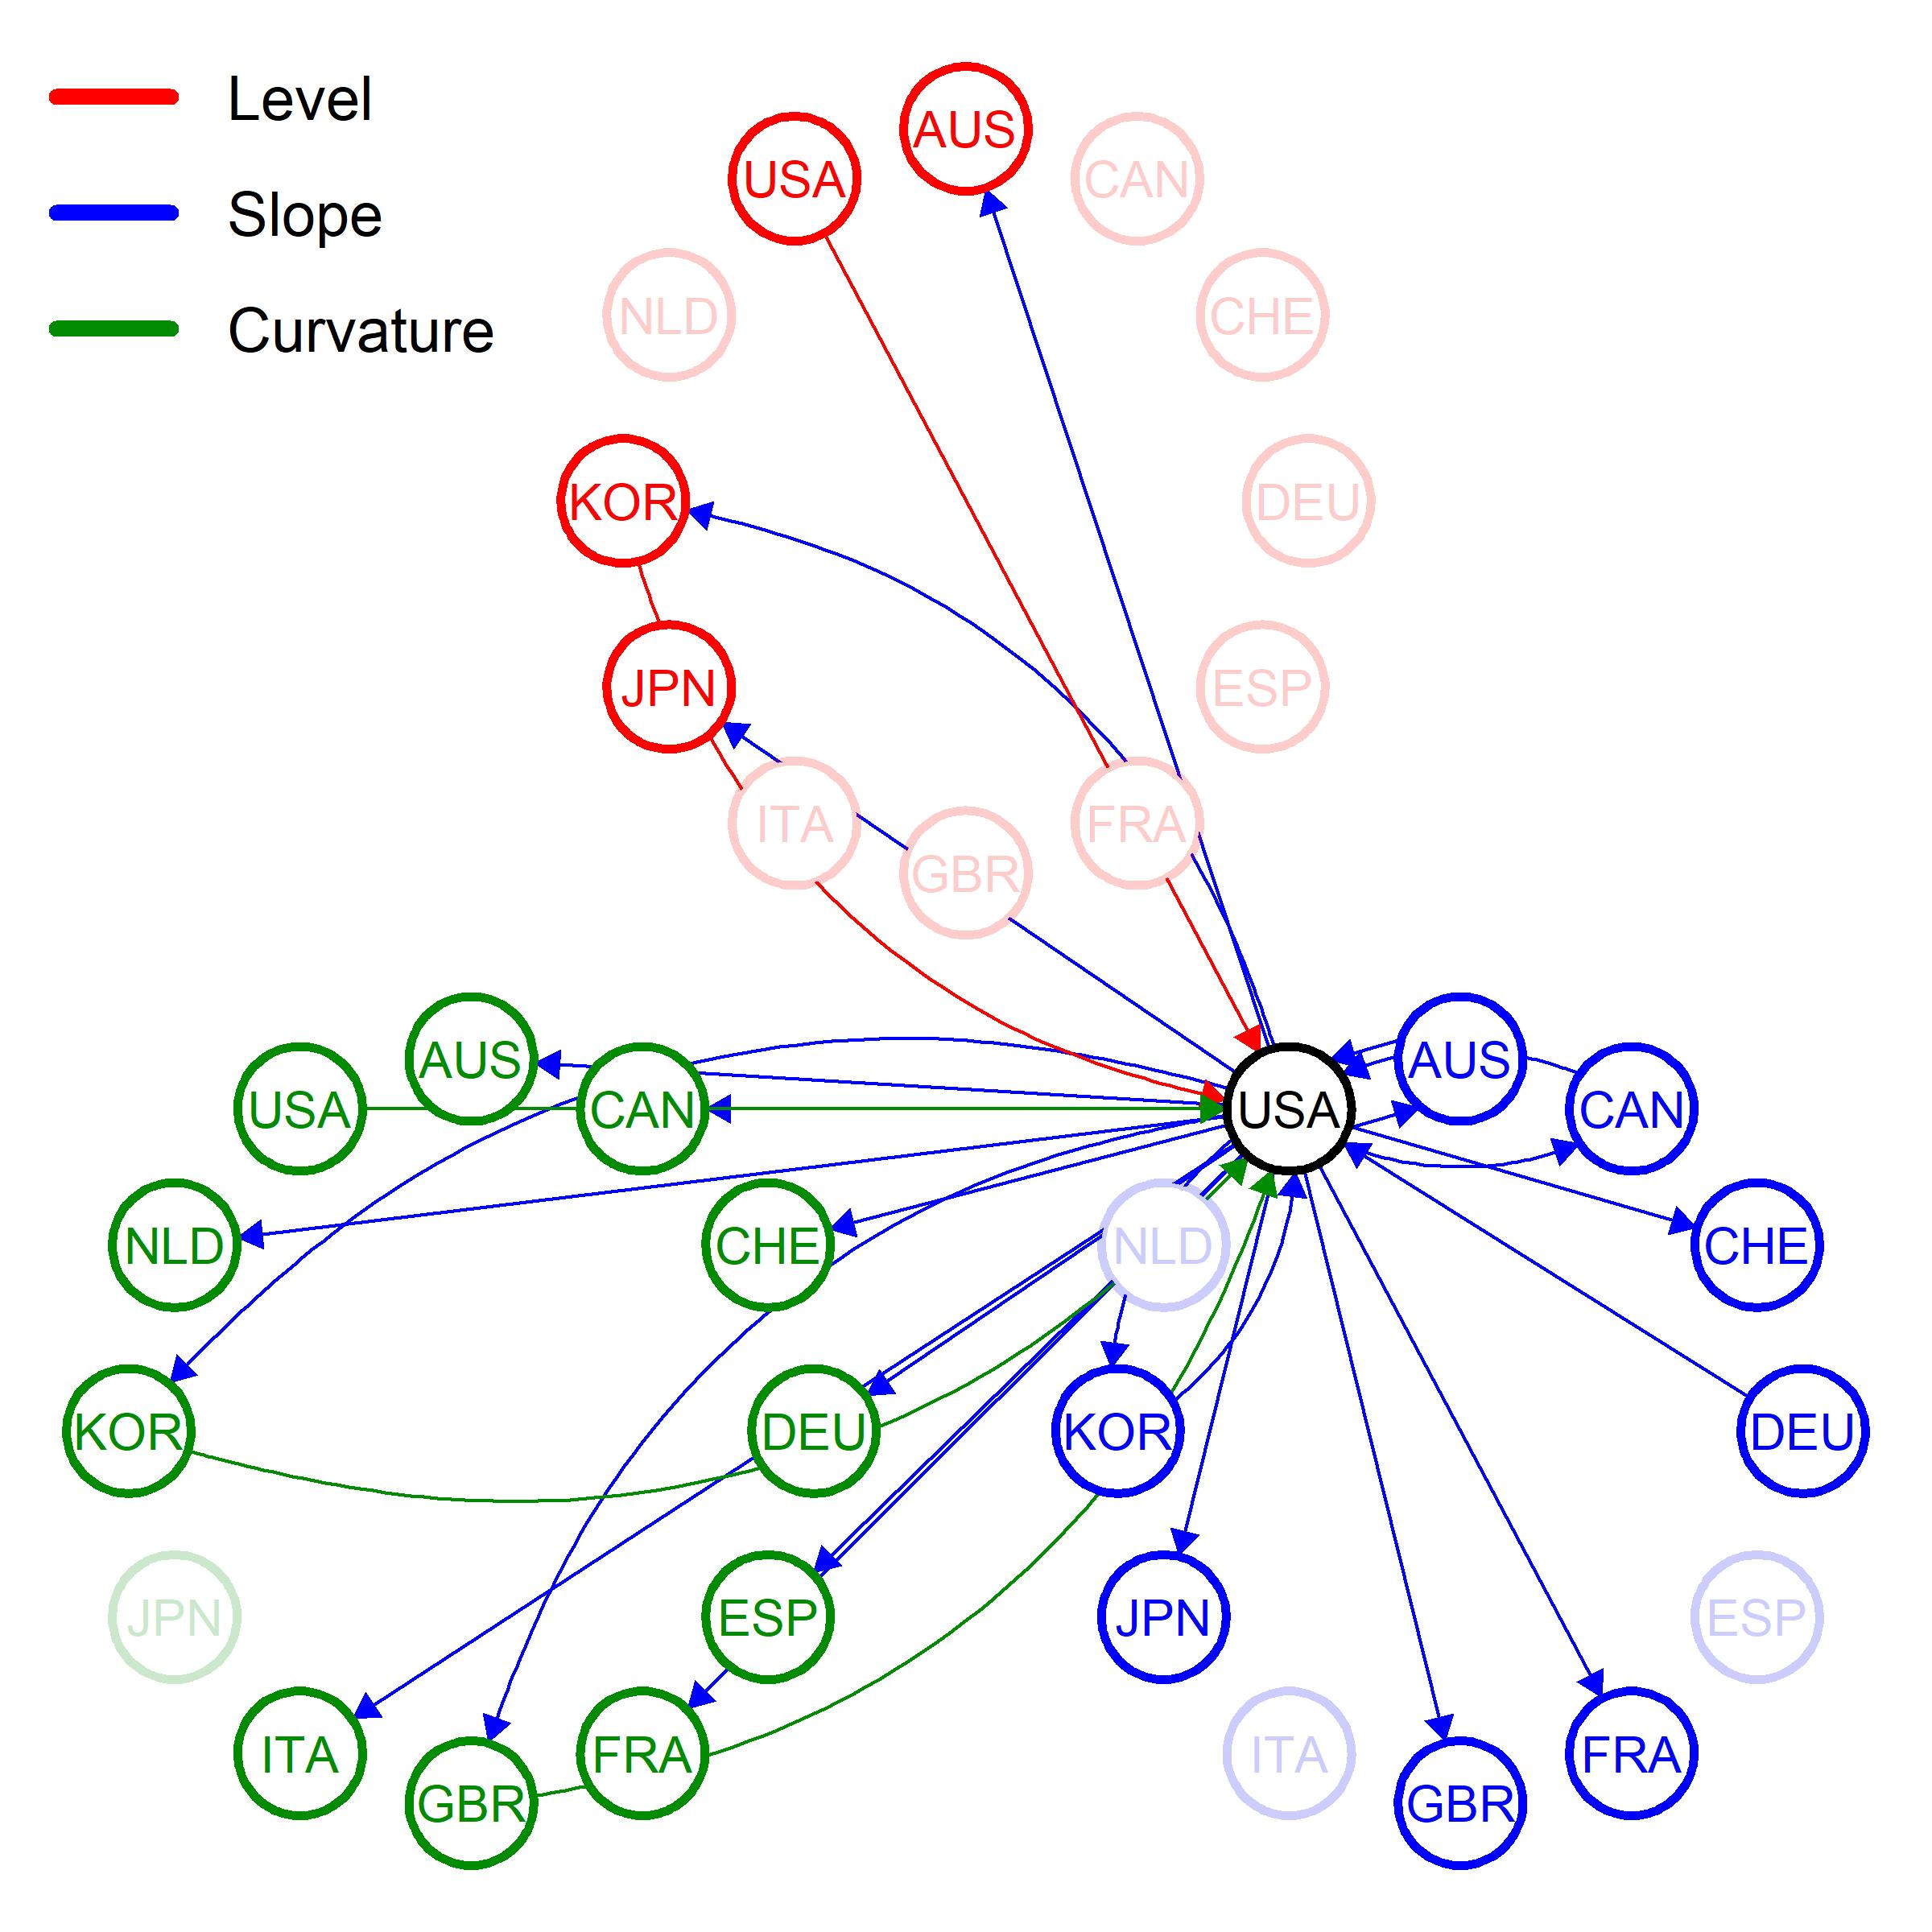
\includegraphics[width=\linewidth]{node_USA_B_2_1998-09-30_2021-12-29_TY_fix}
    \caption{\textbf{USA Slope}}
  \end{subfigure}

  \medskip

\centering
  \begin{subfigure}[t]{.5\textwidth}
    \centering
    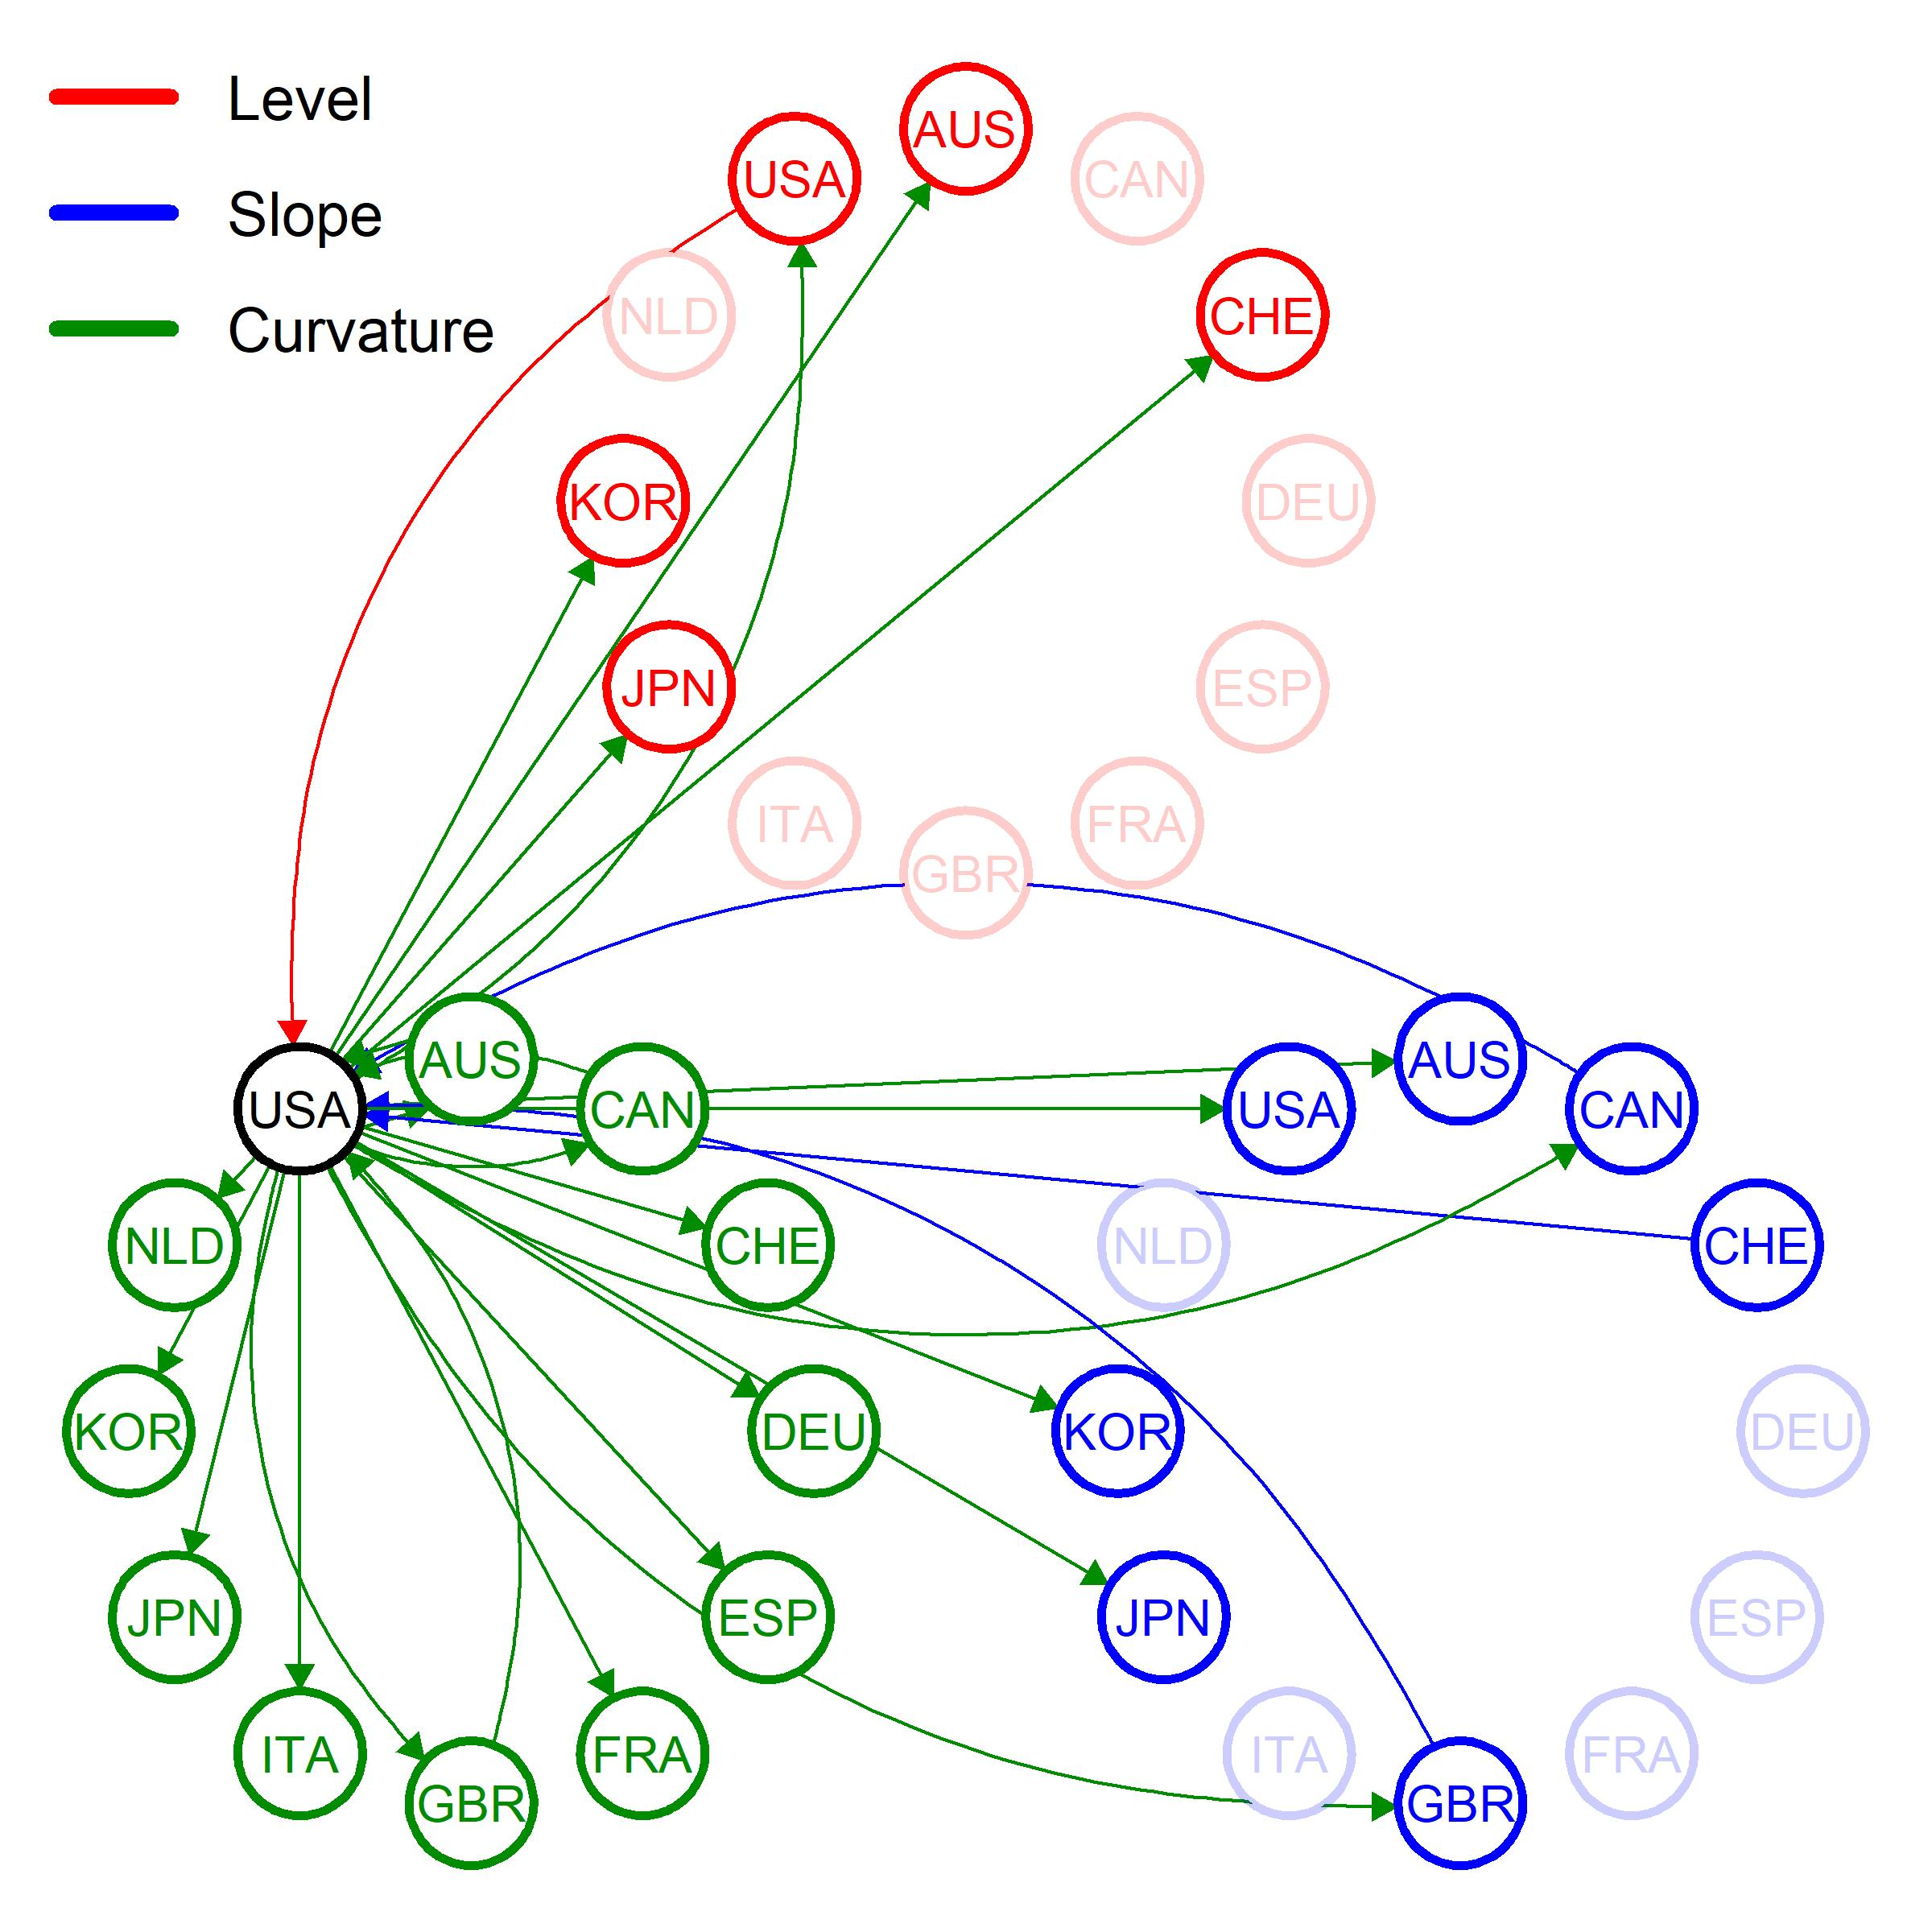
\includegraphics[width=\linewidth]{node_USA_B_3_1998-09-30_2021-12-29_TY_fix}
    \caption{\textbf{USA Curvature}}
  \end{subfigure}
  \hfill

\caption{Interconnectedness in subnetworks}
\label{fig:usaFactors}

\fnote{
In case of the USA Level factor, 31 edges are significant form the total possible 70 which is 44.29\%;

In case of the USA Slope factor, 29 edges are significant form the total possible 70 which is 41.43\%;

In case of the USA Curvature factor, 29 edges are significant form the total possible 70 which is 41.43\%;

}


\end{figure}

%----------------------------------------------------------------------------------------------------------------------------------------------------

\subsection{Time series analysis}

%A statikus vizsgálódás után elvégzem az összekötöttségre vonatkozó dinamikus elemzést is. Gördülő időablakom hosszát 750 napnyinak választom meg. Ez 250 munkanapos évet feltételezve 3 évnek feleltethető meg. Minden egyes eltolással 5 napot ugrok, ami munkanapokat feltételezve egy hetet jelent. Így összesen 659 összekötöttséget reprezentáló modellt illesztek. Az ezekből kapott idősorokat mutatja az 5. ábra. A lila vonal a teljes hálózatra vonatkozó szignifikáns élek hányadát jelenti, a türkiz a különböző faktorok alhálózatainak összegét, míg a sárga a keresztkapcsolatok behúzott éleit jelképezi. A piros hátterű időszak a subprime válságra utal, míg a kék hátterű az európai adósságválságra. A periódusokat \cite{bostanci2020connected} alapján választom meg. Ezekben az időszakokban a hálózat összekötöttségi szintje megnövekszik.

Running a whole sample connectedness analysis may not capture the cyclical and structural changes in the dynamics of linkages. Thus after the static examination we perform a dynamic analysis of the factor interconnectedness. There is no exact role to chose the  sufficient size of sample size period and based on \cite{papana2017financial} and \cite{arce2013credit} we choose a rolling window method with size of 750 observations. Considering 250 business days long years, this can be interpreted as a three year long window. With each shifting we move 5 observations ahead which can be seen as one business week. By doing so, we define 1064 separeted models. 

The time series of summarized (incoming + outgoing) edges resulted by these models are shown on Figure \ref{fig:summarizedEdgeNumbers}. Raddle colored line stands for the ratio of the singnificant edges in the whole newtwork, grey is ratio of the sum of the edges by each subnetwork and yellow represents the ration of the cross connection edges. As stated before, the dotcom bubble is noted by green, the subprime crysis is displayed by the red shaded area, the blue field covers the European sovereign debt and the yellow area displays the period of Covid19.


%--------------------------------------------------------------------------Fig5--------------------------------------------------------------------------
\begin{figure}[H]
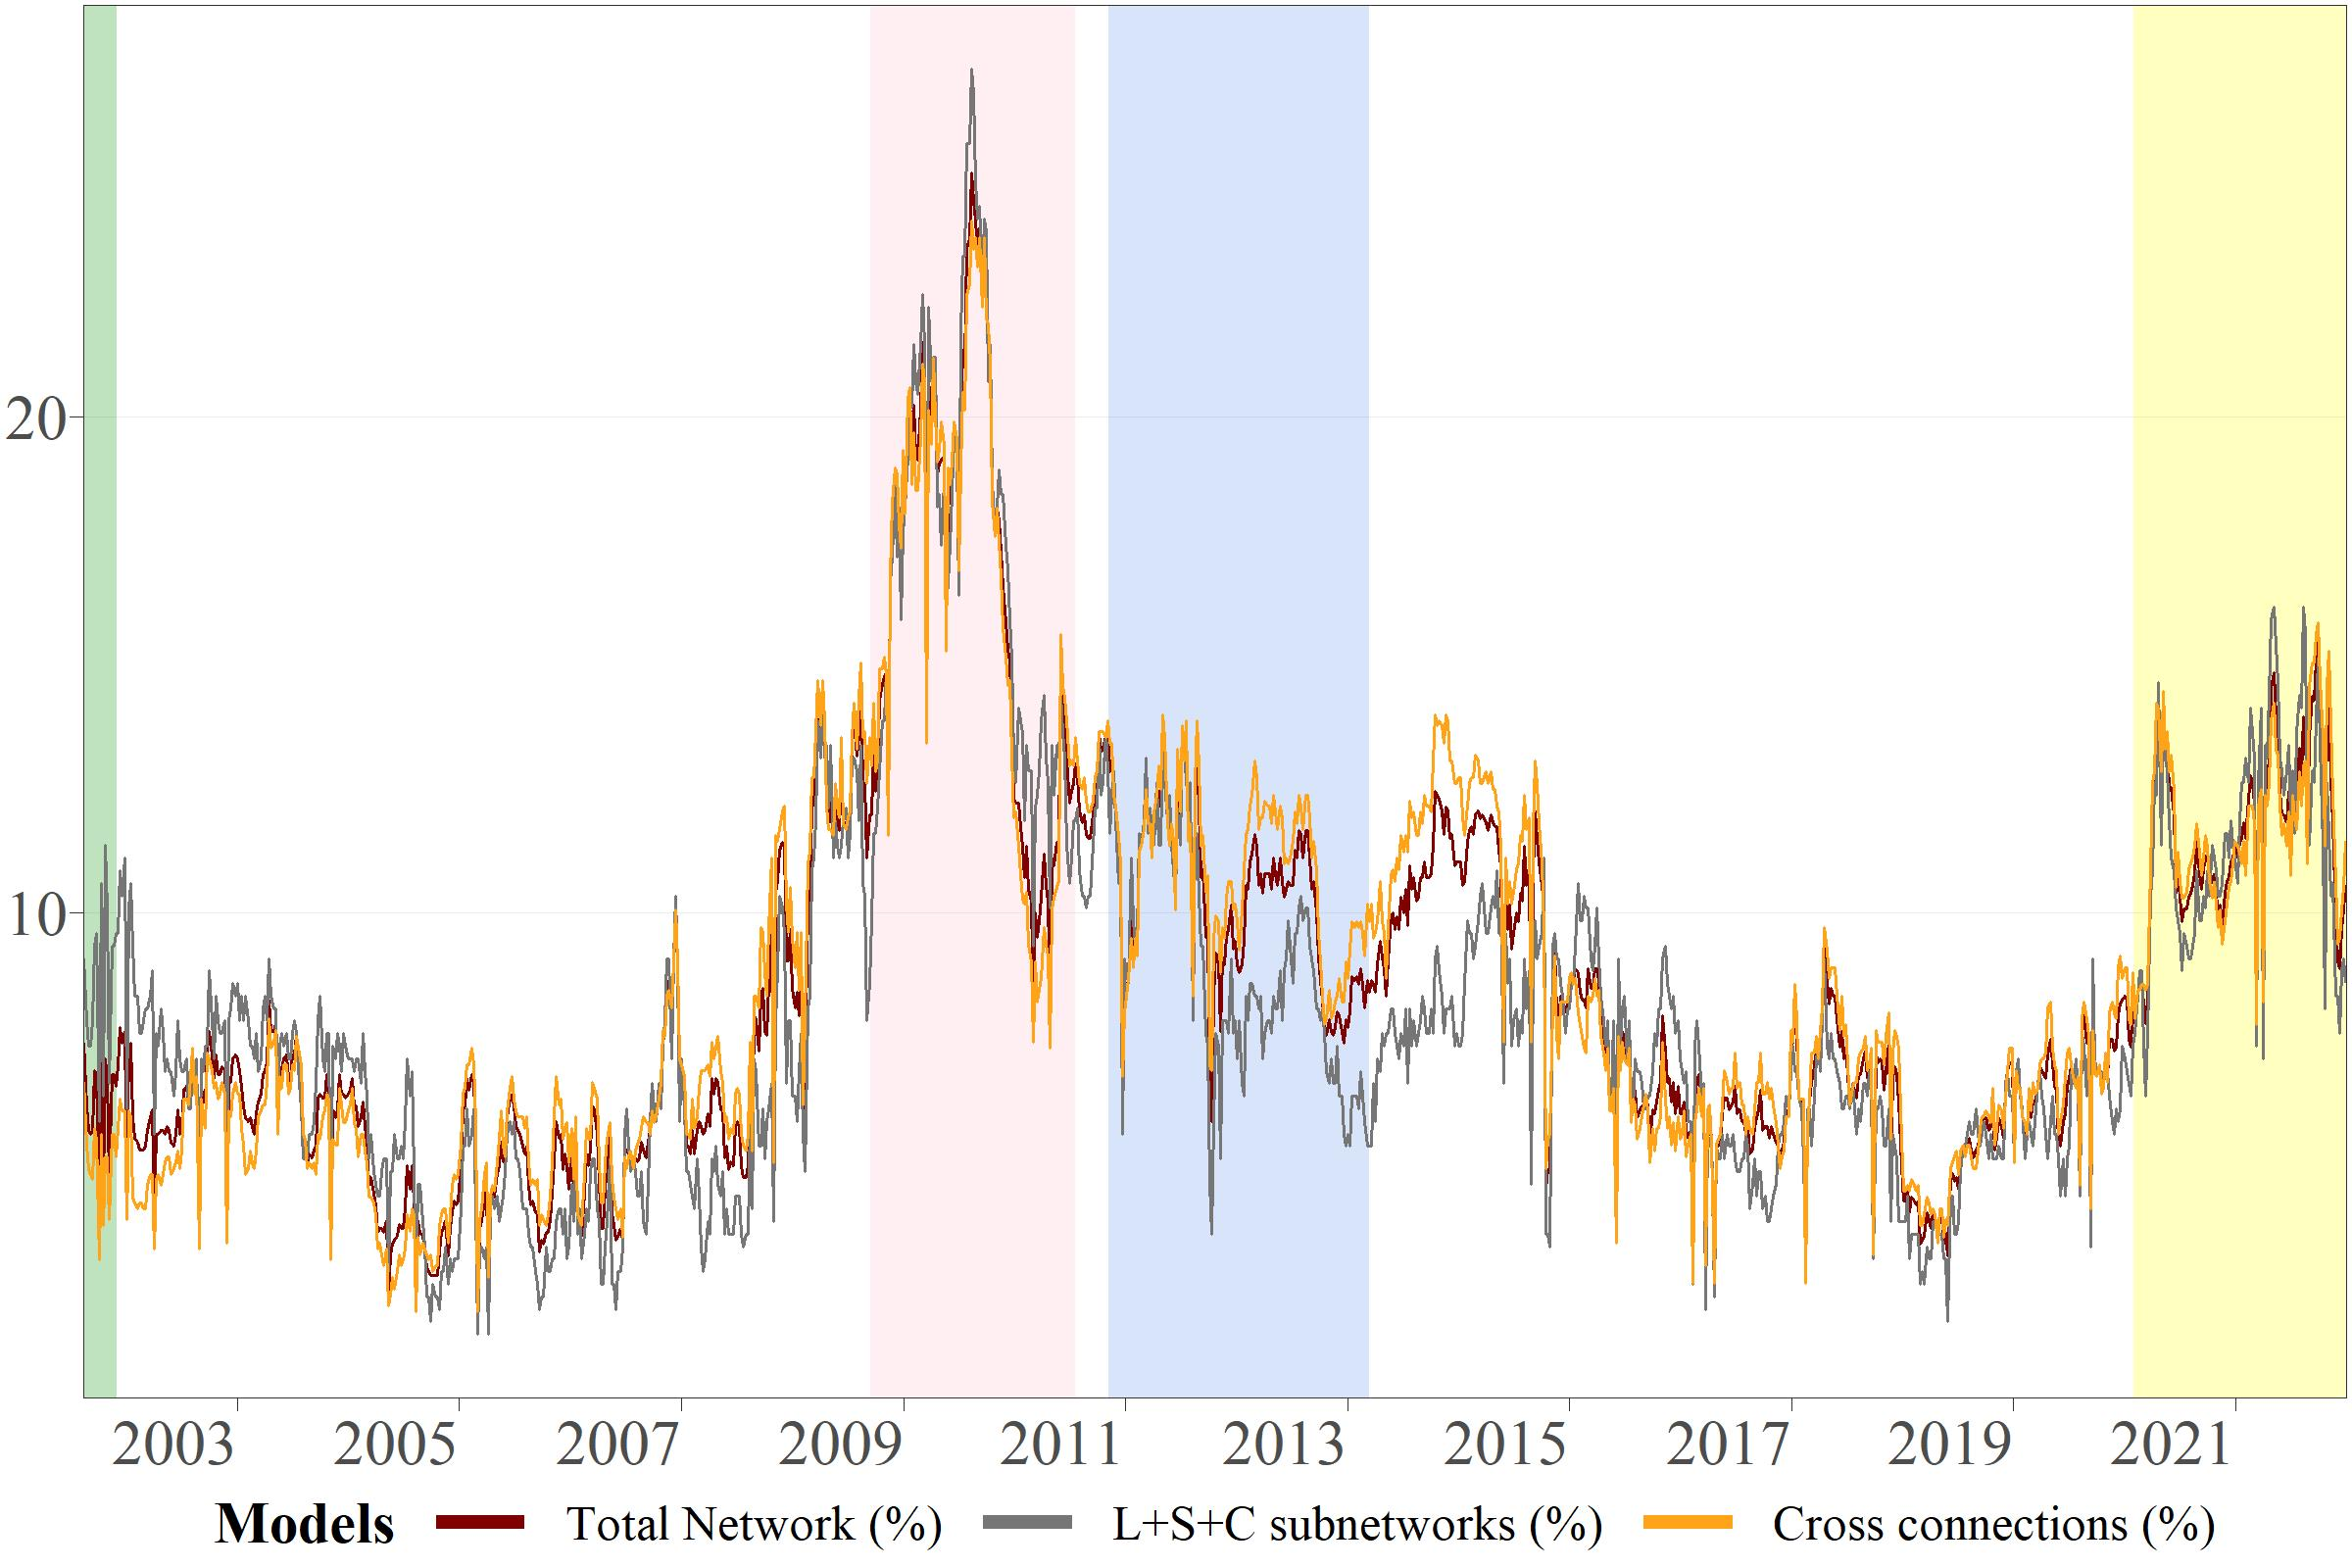
\includegraphics[width=13.5cm]{750edgesDistribution}
\centering

\caption{Summarized edge number by day, resulted by dynamic Toda-Yamamoto analysis}
\label{fig:summarizedEdgeNumbers}
\centering
\fnote{
Raddle colored line: Number of significant edges in the network divided by 1260

\smallskip

Grey colored line: Sum of significant edges within each subnetorks divided by 396 ($3 \times 132$)

\smallskip

Yellow colored line: Sum of significant edges that are defined among the three subnetwork, divided by 896 (1260 - 396)

}
\end{figure}

%A 6. ábra a vizsgált periódus alatt átlagosan letöbb nettósított éllel rendelkező faktorok idősorait mutatja. Ezek növekvő sorrendben: Norvégia Meredekség, USA Görbület és USA Szint. A subprime válság mindhárom faktorra hatással volt, itt az idősorok kiugró értékeket mutatnak. Norvégia Meredekség faktora az európai adósságválság ideje alatt emelkedett meg kimondottan. Ez azzal magyarázható, hogy 2011 végén Norvégia szuverén befektetési alapja eladta a teljes ír és portugál államadósság-állományát, és csökkentette spanyol és olasz kötvényinek tulajdonjogát.

One can see that all three ratios peak during the dotcom period, the subprime crisis and the Covid19 pandemic. There is a consensus in the empirical literature that connectivity measures increase during turbulent periods. Just to name a few, \cite{diebold2009measuring}, \cite{billio2012econometric}, \cite{sowmya2016linkages}, \cite{ahmad2018financial}, all experiences similar behavior. The European sovereign crisis cannot be seen as a worldwide event and only 42\% of the examined population is part of the euro-zone. Hence the graphs do not show upward tendency during this period. We split the whole time horizon to 7 subperiods, 4 turbulent ones (shaded areas on Figure \ref{fig:summarizedEdgeNumbers}) and 3 calm phases (white areas on Figure \ref{fig:summarizedEdgeNumbers}). Table \ref{tab:periods} contains the average sumrized edges where the denominator is the number of observations within the given term. 


\begin{table}[H]
\fontsize{10}{10}\selectfont
\centering% centering table
\begin{tabular}{l  cccccccc}% creating eight columns
\hline\hline \\ [-1.5ex]                         %inserting double-line


				& Whole period  &Dotcom	&1. calm  & Subprime & 2. calm &Sovereign & 3. calm & Covid19 \\
\hline \\ [-1.5ex]  
Level			&9.8 &7.2		&6.6		&22.1			&12.0		&10.5		&8.0	&15.4\\
Slope			&11.3 &12.6		&8.3		&23.5			&19.4		&16.6		&8.5		&12.4\\
Curvature		&11.3 &14.4		&9.4	&21.8		&15.1			&8.0		&9.4		&17.1\\
Cross connections	&75.5 &43.4		&54.3	&139.7	&112.0		&93.1		&65.9		&100.3\\
All edges		&108.0 &77.6		&78.6		&207.1		&158.4	&128.2	&91.8		&145.3\\

%----------------------------------------------------------------------------------------------------------------------------------------------------

\hline            
\end{tabular}
\caption{Average edge count by edges during the seven sub-periods - 750 observations long window size} %title of the table
\label{tab:periods}
\end{table}


Table \ref{tab:periods} also proves that in crisis periods, significant edges for all three individual factors increases. European Sovereign crisis is an exception, during this phase further decrease in edge numbers is observed. This also confirms that this crisis was not worldwide, howeverit has significant effects on a subset of the countries. Table \ref{tab:euroEdges} in the Appendix shows the same subsetting only for the chosen eurozone countries (DEU, ITA, ESP, FRA, NDL). Except for Curvature the number of edges peaks during the European sovereig crisis during this time.

\medskip

So far the sum of the edges have been examined. We also check the net edges (outgoing - incoming) and find that the system is driven by the American factors. During the 1064 observation long examination period the USA Level has the highest amount of net edges (4114), followed by the USA Curvature (3408) and the USA Slope (2539). The time series of these factors are shown on Figure \ref{fig:usaNodes}.

\begin{figure}[H]
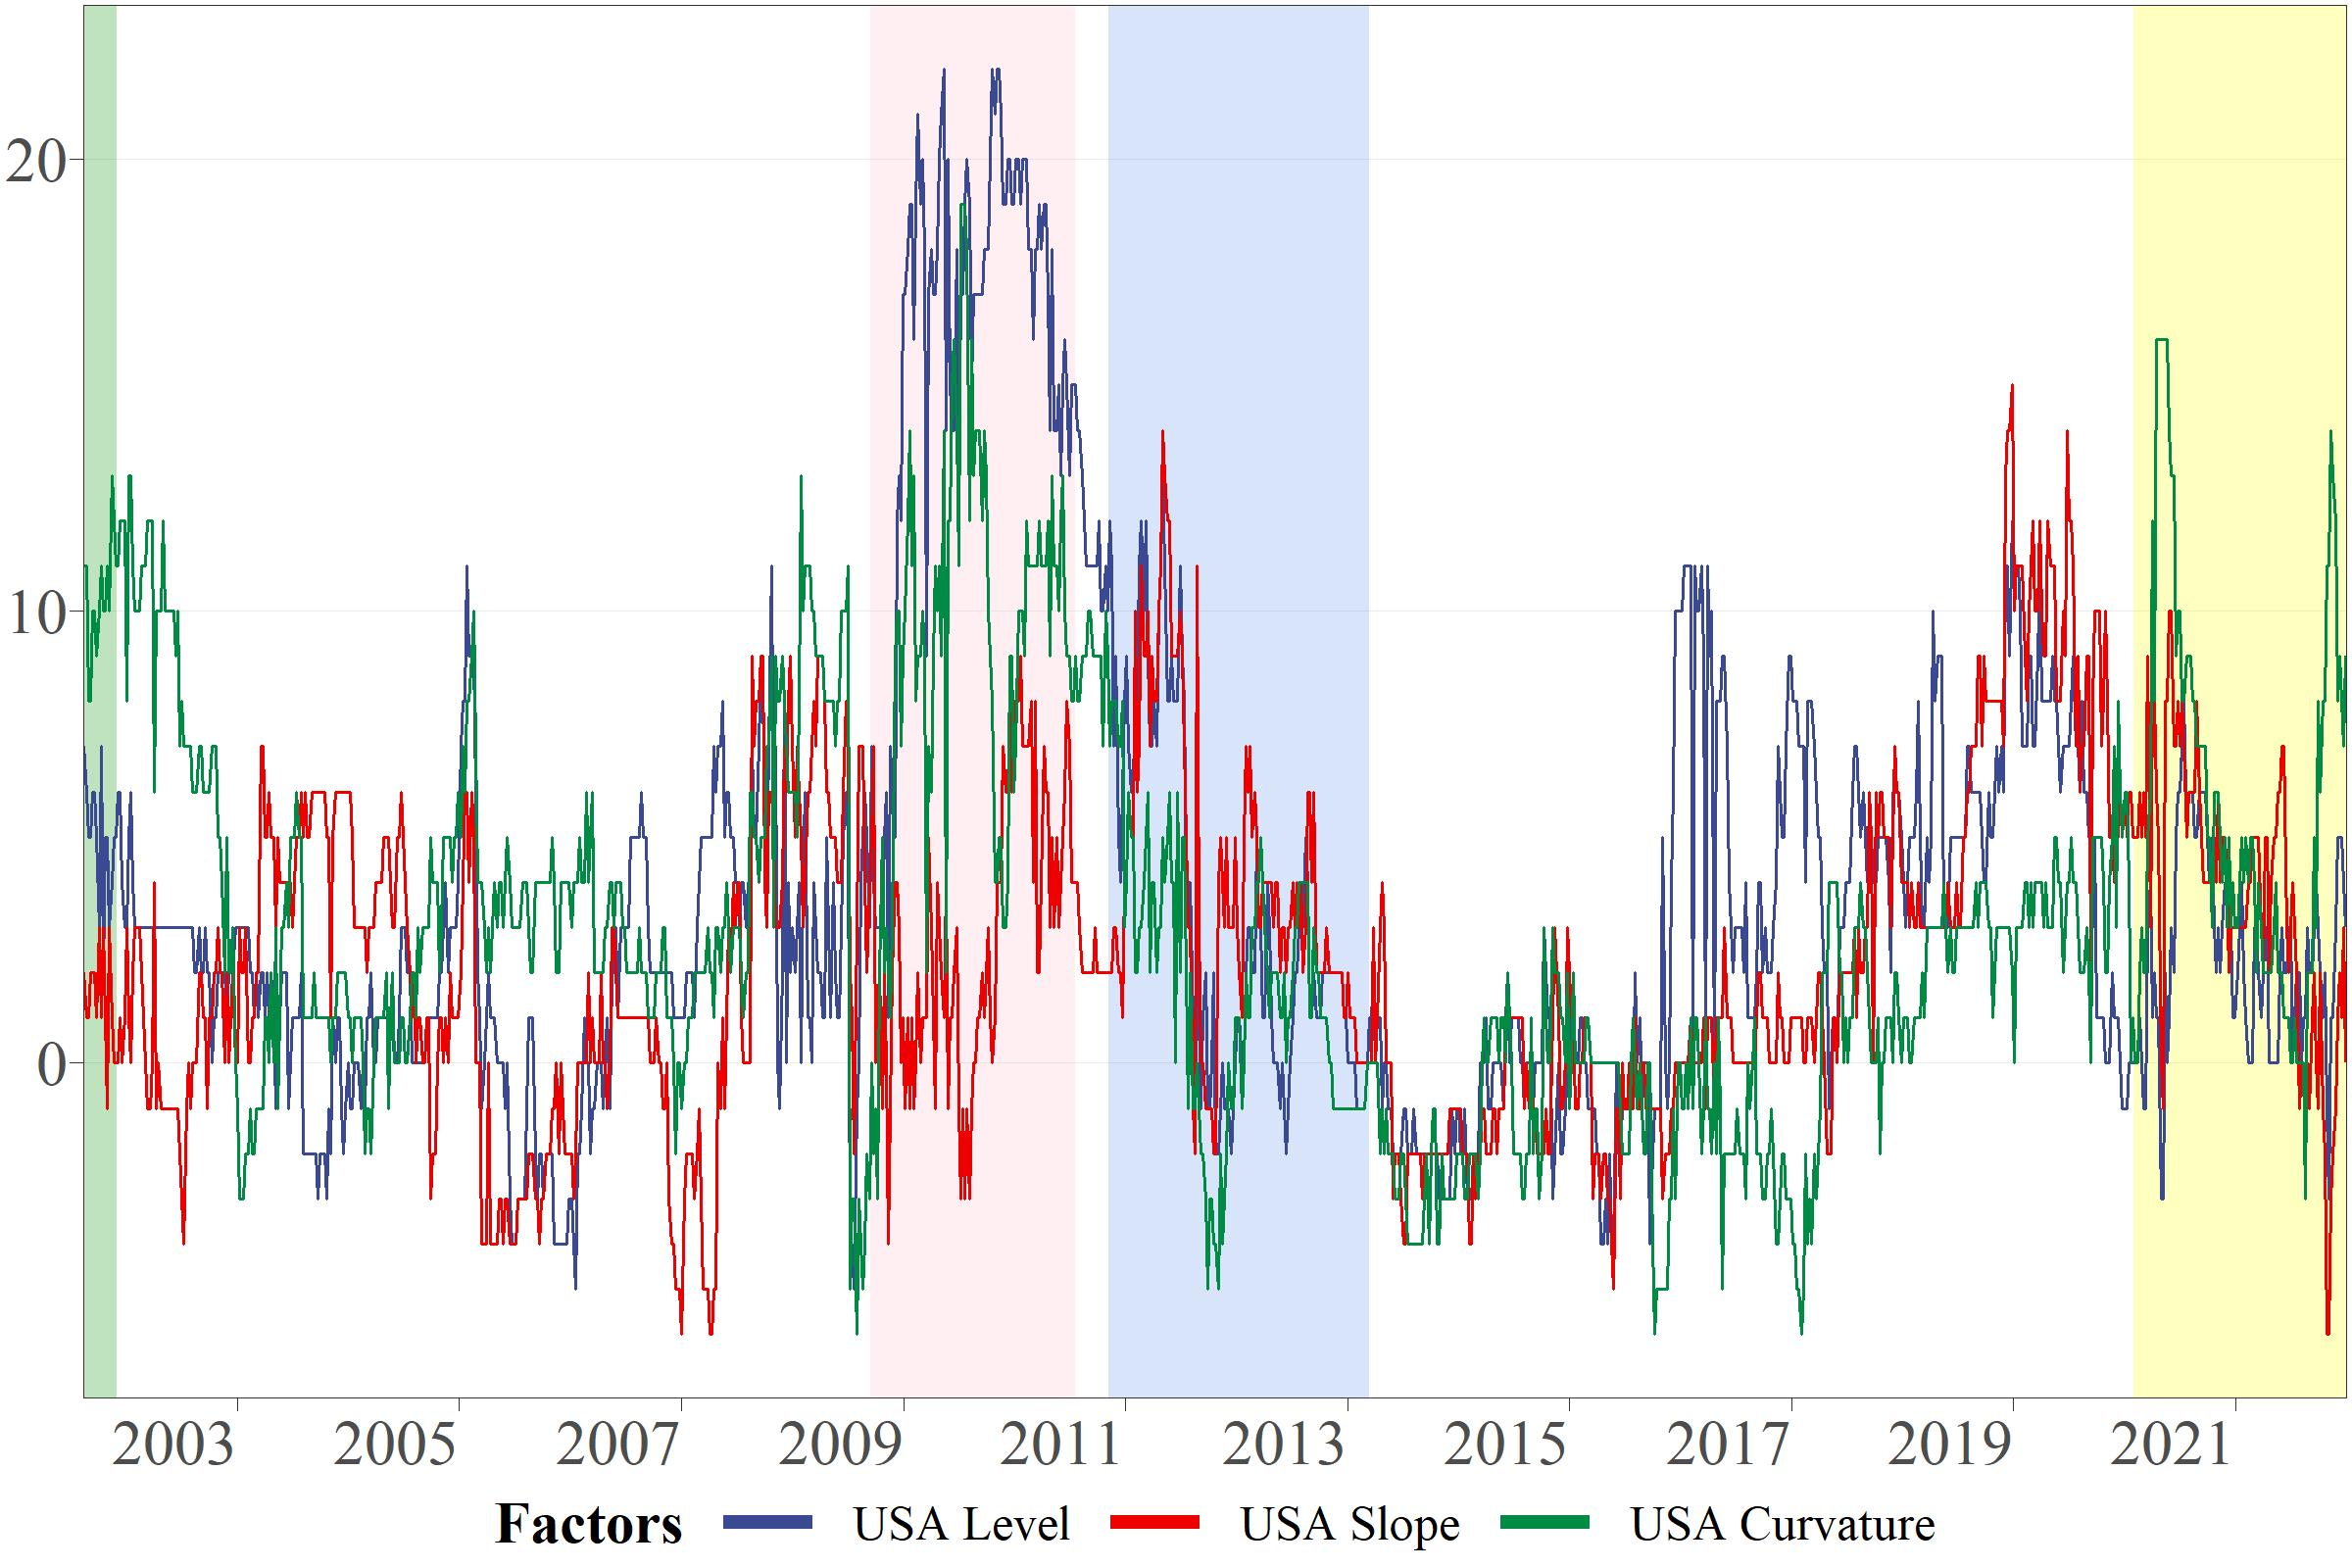
\includegraphics[width=13.5cm]{USA nodes}
\centering

\caption{Summarized edge number by day, resulted by dynamic Toda-Yamamoto analysis }
\label{fig:usaNodes}
\centering
\fnote{
Widnow size: 750, Lag: based on AIC
}
\end{figure}

The net edge count of Level factors peaked during the subprime crisis and there was a local maximum during the European sovereign crisis too. This is in line with \cite{braun1995good} who points out that thanks to bad news, cross market correlations increase. Also another local maximum can be seen between 2016 and 2017. There are several events that increases the number of connections for the Slope of the USA. On 2016 July 8, the 10-year treasury note settles on 1.366\% which is the lowest during the observation period (so far.) On November 8 Donald Trump is elected as president. On December 14 Fed announces interest rate increase then on 2017 March 17 Fed rises rates again.

The net Slope edges first peaked during the period of 2006-2007. The plot provides an early warning signals for the subprime crisis which is in line with the findings of \cite{estrella1991term}. The number of connections decreased with the early stage of the subprime crisis then increased significantly.
crisis period and increased substantially after the global financial crisis. Between the European sovereign crisis and the Covid19 pandemic there is an upward pointing trend in the number of such edges. This can be interpreted as a convergence of monetary policies through the elements of the network during this period, since Slope reflect the state of monetary policy.

\cite{dewachter2006macro} and \cite{diebold2006forecasting} determine that Curvature is less linked to macroeconomic fundamentals and shocks. According to \cite{abbritti2013global} Curvature is related to the current stance of monetary policy explains the variation in interest rates across maturities.
Apparently the net number of Curvature connections is sensitive to the Fed interest rate changes. Between 2001 and 2003 Fed fund rate drops from 6.5\% to 1\%. This is the first period Curvature graph peaks on Figure 5. There is a local maximum in 2005 which represents the 2004-2006 rate hike. Similarly to the dotcom period, from 2007 September to 2008 December the rate drops from 4.75\% to 0.25\%. The subprime crisis is the period when the curvature graph peaks. There are minor increases in edge number thanks to the 2015-2018 rate hikes, but the 2020 March 3 and 14-15 Fed emergency meetings make Curvature edge counts peak again in the early phase of Covid19 pandemic. 

\medskip 

Table 6 identifies the role of a country yield curve factor for each associated time period. Minus sign indicates that the factor is a net recipent of edges while plus sign stands for being net provider. One can see that all three factors of the USA are net providers in every periods. This a further proof of the result of \cite{brusa2020one} about Fed being in a unique driving role of the global bond market. Besides USA, Canadian Level and Slope have strong driving potential in most of the periods. It is arguable that this role is a result of close dependencies with the States. For example \cite{greenwood2015measuring} document that Canada being a member of NAFTA (North American Free Trade Agreement) can be an indicator of being net positive in most of the cases. 

Besides the North-American continet, German and Swiss Level are being mostly (especially in crisis period) net provider. Additionally Korean yield curve factors are being mostly positive. 

These results are confirmed by a robostness check by chosing 500 and 1000 observation to our rolling window. Table 10 in the Appendix shows the roles of the factors. Comparing to the 750 window size, the results are identical in 70.2\% for the 500 window and identical in 78.7\% in case of the 1000 window.


\begin{table}[H]
\fontsize{10}{10}\selectfont
\centering% centering table
\begin{tabular}{l  cccccccc}% creating eight columns
\hline\hline \\ [-1.5ex]                         %inserting double-line


	& \rot{Whole period}  &\rot{Dotcom}	&\rot{1. calm}  & \rot{Subprime} & \rot{2. calm} & \rot{Sovereign} & \rot{3. calm} & \rot{Covid19} \\
\hline \\ [-1.5ex]  
AUS L	&\cellcolor{red!25}-	&\cellcolor{red!25}-	&\cellcolor{red!25}-	&\cellcolor{red!25}-	&\cellcolor{red!25}-	&\cellcolor{red!25}-	&\cellcolor{red!25}-	&\cellcolor{red!25}-	 \\
CAN L	&\cellcolor{green!25}+	&\cellcolor{green!25}+	&\cellcolor{green!25}+	&\cellcolor{red!25}-	&\cellcolor{red!25}-	&\cellcolor{green!25}+	&\cellcolor{green!25}+	&\cellcolor{green!25}+   \\
CHE L	&\cellcolor{green!25}+	&\cellcolor{green!25}+	&\cellcolor{green!25}+	&\cellcolor{green!25}+	&\cellcolor{green!25}+	&\cellcolor{green!25}+	&\cellcolor{green!25}+	&\cellcolor{green!25}+   \\
DEU L	&\cellcolor{green!25}+	&\cellcolor{red!25}-	&\cellcolor{green!25}+	&\cellcolor{green!25}+	&\cellcolor{green!25}+	&\cellcolor{green!25}+	&\cellcolor{red!25}-	&\cellcolor{green!25}+   \\
ESP L	&\cellcolor{green!25}+	&\cellcolor{red!25}-	&\cellcolor{red!25}-	&\cellcolor{green!25}+	&\cellcolor{green!25}+	&\cellcolor{red!25}-	&\cellcolor{green!25}+	&\cellcolor{green!25}+   \\
FRA L	&\cellcolor{red!25}-	&\cellcolor{red!25}-	&\cellcolor{green!25}+	&\cellcolor{red!25}-	&\cellcolor{red!25}-	&\cellcolor{red!25}-	&\cellcolor{green!25}+	&\cellcolor{red!25}-     \\
GBR L	&\cellcolor{red!25}-	&\cellcolor{red!25}-	&\cellcolor{red!25}-	&\cellcolor{red!25}-	&\cellcolor{red!25}-	&\cellcolor{red!25}-	&\cellcolor{red!25}-	&\cellcolor{green!25}+   \\
ITA L	&\cellcolor{green!25}+	&\cellcolor{green!25}+	&\cellcolor{green!25}+	&\cellcolor{green!25}+	&\cellcolor{red!25}-	&\cellcolor{red!25}-	&\cellcolor{yellow!25}0	&\cellcolor{green!25}+   \\
JPN L	&\cellcolor{green!25}+	&\cellcolor{green!25}+	&\cellcolor{green!25}+	&\cellcolor{green!25}+	&\cellcolor{red!25}-	&\cellcolor{red!25}-	&\cellcolor{red!25}-	&\cellcolor{green!25}+   \\
KOR L	&\cellcolor{green!25}+	&\cellcolor{green!25}+	&\cellcolor{green!25}+	&\cellcolor{green!25}+	&\cellcolor{red!25}-	&\cellcolor{green!25}+	&\cellcolor{green!25}+	&\cellcolor{green!25}+   \\
NLD L	&\cellcolor{red!25}-	&\cellcolor{green!25}+	&\cellcolor{red!25}-	&\cellcolor{red!25}-	&\cellcolor{green!25}+	&\cellcolor{red!25}-	&\cellcolor{red!25}-	&\cellcolor{red!25}-     \\
USA L	&\cellcolor{green!25}+	&\cellcolor{green!25}+	&\cellcolor{green!25}+	&\cellcolor{green!25}+	&\cellcolor{green!25}+	&\cellcolor{green!25}+	&\cellcolor{green!25}+	&\cellcolor{green!25}+   \\
AUS S	&\cellcolor{red!25}-	&\cellcolor{red!25}-	&\cellcolor{red!25}-	&\cellcolor{green!25}+	&\cellcolor{red!25}-	&\cellcolor{red!25}-	&\cellcolor{red!25}-	&\cellcolor{red!25}-     \\
CAN S	&\cellcolor{green!25}+	&\cellcolor{green!25}+	&\cellcolor{green!25}+	&\cellcolor{green!25}+	&\cellcolor{green!25}+	&\cellcolor{green!25}+	&\cellcolor{green!25}+	&\cellcolor{green!25}+   \\
CHE S	&\cellcolor{green!25}+	&\cellcolor{green!25}+	&\cellcolor{green!25}+	&\cellcolor{red!25}-	&\cellcolor{red!25}-	&\cellcolor{red!25}-	&\cellcolor{red!25}-	&\cellcolor{green!25}+   \\
DEU S	&\cellcolor{green!25}+	&\cellcolor{green!25}+	&\cellcolor{green!25}+	&\cellcolor{green!25}+	&\cellcolor{green!25}+	&\cellcolor{red!25}-	&\cellcolor{red!25}-	&\cellcolor{red!25}-     \\
ESP S	&\cellcolor{red!25}-	&\cellcolor{red!25}-	&\cellcolor{red!25}-	&\cellcolor{green!25}+	&\cellcolor{green!25}+	&\cellcolor{green!25}+	&\cellcolor{red!25}-	&\cellcolor{green!25}+   \\
FRA S	&\cellcolor{red!25}-	&\cellcolor{red!25}-	&\cellcolor{red!25}-	&\cellcolor{red!25}-	&\cellcolor{red!25}-	&\cellcolor{red!25}-	&\cellcolor{green!25}+	&\cellcolor{red!25}-     \\
GBR S	&\cellcolor{red!25}-	&\cellcolor{green!25}+	&\cellcolor{green!25}+	&\cellcolor{red!25}-	&\cellcolor{green!25}+	&\cellcolor{red!25}-	&\cellcolor{red!25}-	&\cellcolor{red!25}-     \\
ITA S	&\cellcolor{red!25}-	&\cellcolor{red!25}-	&\cellcolor{red!25}-	&\cellcolor{red!25}-	&\cellcolor{red!25}-	&\cellcolor{green!25}+	&\cellcolor{red!25}-	&\cellcolor{red!25}-     \\
JPN S	&\cellcolor{red!25}-	&\cellcolor{red!25}-	&\cellcolor{red!25}-	&\cellcolor{red!25}-	&\cellcolor{red!25}-	&\cellcolor{red!25}-	&\cellcolor{red!25}-	&\cellcolor{red!25}-     \\
KOR S	&\cellcolor{red!25}-	&\cellcolor{red!25}-	&\cellcolor{green!25}+	&\cellcolor{red!25}-	&\cellcolor{green!25}+	&\cellcolor{green!25}+	&\cellcolor{green!25}+	&\cellcolor{green!25}+   \\
NLD S	&\cellcolor{red!25}-	&\cellcolor{green!25}+	&\cellcolor{red!25}-	&\cellcolor{red!25}-	&\cellcolor{green!25}+	&\cellcolor{red!25}-	&\cellcolor{red!25}-	&\cellcolor{green!25}+   \\
USA S	&\cellcolor{green!25}+	&\cellcolor{green!25}+	&\cellcolor{green!25}+	&\cellcolor{green!25}+	&\cellcolor{green!25}+	&\cellcolor{green!25}+	&\cellcolor{green!25}+	&\cellcolor{green!25}+   \\
AUS C	&\cellcolor{red!25}-	&\cellcolor{red!25}-	&\cellcolor{green!25}+	&\cellcolor{red!25}-	&\cellcolor{red!25}-	&\cellcolor{green!25}+	&\cellcolor{red!25}-	&\cellcolor{red!25}-     \\
CAN C	&\cellcolor{red!25}-	&\cellcolor{red!25}-	&\cellcolor{red!25}-	&\cellcolor{red!25}-	&\cellcolor{green!25}+	&\cellcolor{green!25}+	&\cellcolor{red!25}-	&\cellcolor{red!25}-     \\
CHE C	&\cellcolor{red!25}-	&\cellcolor{green!25}+	&\cellcolor{red!25}-	&\cellcolor{green!25}+	&\cellcolor{red!25}-	&\cellcolor{red!25}-	&\cellcolor{green!25}+	&\cellcolor{red!25}-     \\
DEU C	&\cellcolor{red!25}-	&\cellcolor{red!25}-	&\cellcolor{red!25}-	&\cellcolor{green!25}+	&\cellcolor{red!25}-	&\cellcolor{green!25}+	&\cellcolor{red!25}-	&\cellcolor{red!25}-     \\
ESP C	&\cellcolor{red!25}-	&\cellcolor{red!25}-	&\cellcolor{red!25}-	&\cellcolor{red!25}-	&\cellcolor{red!25}-	&\cellcolor{red!25}-	&\cellcolor{red!25}-	&\cellcolor{green!25}+   \\
FRA C	&\cellcolor{red!25}-	&\cellcolor{red!25}-	&\cellcolor{red!25}-	&\cellcolor{red!25}-	&\cellcolor{red!25}-	&\cellcolor{green!25}+	&\cellcolor{green!25}+	&\cellcolor{red!25}-     \\
GBR C	&\cellcolor{red!25}-	&\cellcolor{green!25}+	&\cellcolor{red!25}-	&\cellcolor{green!25}+	&\cellcolor{yellow!25}0	&\cellcolor{red!25}-	&\cellcolor{red!25}-	&\cellcolor{red!25}-     \\
ITA C	&\cellcolor{red!25}-	&\cellcolor{red!25}-	&\cellcolor{red!25}-	&\cellcolor{red!25}-	&\cellcolor{red!25}-	&\cellcolor{red!25}-	&\cellcolor{red!25}-	&\cellcolor{red!25}-     \\
JPN C	&\cellcolor{green!25}+	&\cellcolor{green!25}+	&\cellcolor{green!25}+	&\cellcolor{red!25}-	&\cellcolor{red!25}-	&\cellcolor{green!25}+	&\cellcolor{green!25}+	&\cellcolor{red!25}-     \\
KOR C	&\cellcolor{green!25}+	&\cellcolor{green!25}+	&\cellcolor{green!25}+	&\cellcolor{green!25}+	&\cellcolor{green!25}+	&\cellcolor{green!25}+	&\cellcolor{green!25}+	&\cellcolor{red!25}-     \\
NLD C	&\cellcolor{red!25}-	&\cellcolor{red!25}-	&\cellcolor{red!25}-	&\cellcolor{red!25}-	&\cellcolor{red!25}-	&\cellcolor{green!25}+	&\cellcolor{red!25}-	&\cellcolor{red!25}-     \\
USA C	&\cellcolor{green!25}+	&\cellcolor{green!25}+	&\cellcolor{green!25}+	&\cellcolor{green!25}+	&\cellcolor{green!25}+	&\cellcolor{green!25}+	&\cellcolor{green!25}+	&\cellcolor{green!25}+   \\
%----------------------------------------------------------------------------------------------------------------------------------------------------

\hline            
\end{tabular}
\caption{redgreen} %title of the table
\end{table}











%-----------------------------------------------------------------------------------table6------------------------------------------------------------------

%\begin{table}[H]
%\fontsize{10}{10}\selectfont
%\centering% centering table
%\begin{tabular}{l | cccccc}% creating eight columns
%\hline\hline \\ [-1.5ex]                         %inserting double-line


%		& 	Whole period  &	1. calm	&	1. crisis& 	2. calm& 	2. crisis&	 3. calm \\
%\hline \\ [-1.5ex]  
%Level	&		29	&	7	&	16.2	&	13.4	&  	12.1	&	 12\\
%Slope	&		41	&	6	&	25.5	&	22.5	& 	16.2	& 	8.6\\
%Curvature	&	23	&	7.3	&	20.7	&	9.7	& 	9.2	&	 9.9\\
%Cross connections	&		225	&	61.8	&	142.2	&	109.1	& 	101.2	& 	76.1\\
%----------------------------------------------------------------------------------------------------------------------------------------------------

%\hline            
%\end{tabular}
%\label{table:nonlin}% is used to refer this table in the text
%\caption{Average edge count by edges during the five sub-periods - 750 observations long window size} %title of the table


%\end{table}


\section{Robostness checks}

\subsection{Changing window size}

To provide stronger arguments we implement two types of robustness checks. First we run calculate the edge numbers for each periods with 500 and 1000 rolling window size. We devided the sum of edges by the observation count in the given period to get the average edge count per period for each factor types. The results are highlighted in Table \ref{tab:differentWindowSizes}. Since our data starts at 9/30/1998 the 1000 observation long rolling window method cannot interpret the dotcom bubble, therefore only six sub-period is identified in this case. 

\begin{table}[H]

\fontsize{10}{10}\selectfont
\centering% centering table
\captionsetup{justification=centering}

\begin{subtable}[t]{1\textwidth}
\centering% centering table
\begin{tabular}{l  cccccccc}% creating eight columns
\hline\hline \\ [-1.5ex]                         %inserting double-line


				& Whole period  &Dotcom	&1. calm  & Subprime & 2. calm &Sovereign & 3. calm & Covid19 \\
\hline \\ [-1.5ex]  
Level				&7.5	&6.7	&6.0		&15.0	&8.0	&6.0		&7.0		&10.0   \\
Slope				&8.4	&10.9	&6.8		&15.5	&9.1	&6.3		&8.0		&9.0    \\
Curvature			&8.1	&13.7	&6.9		&8.8	&8.7	&7.5		&8.1		&8.7    \\
Cross connections	&55.9	&57.5	&47.0		&84.7	&61.4	&55.0		&52.0		&72.6   \\
All edges			&79.9	&88.7	&66.7		&124.0	&87.1	&74.7		&75.1		&100.4	\\

%----------------------------------------------------------------------------------------------------------------------------------------------------

\hline            
\end{tabular}
\caption{\textbf{Average edge count by factor types during the whole period the seven sub-periods - 500 observations long window size}} %title of the table
\end{subtable}
\hspace{\fill}

\bigskip 


\begin{subtable}[t]{1\textwidth}
\centering% centering table
\begin{tabular}{l  cccccccc}% creating eight columns
\hline\hline \\ [-1.5ex]                         %inserting double-line


				& Whole period  &Dotcom	&1. calm  & Subprime & 2. calm &Sovereign & 3. calm & Covid19 \\
\hline \\ [-1.5ex]  
Level				&9.8	&7.2	&6.6		&22.1	&12.0	&10.5		&8.0		&15.4   \\
Slope				&11.3	&12.6	&8.3		&23.5	&19.4	&16.6		&8.5		&12.4   \\
Curvature			&11.3	&14.4	&9.4		&21.8	&15.1	&8.0		&9.4		&17.1   \\
Cross connections	&75.5	&43.4	&54.3		&139.7	&112.0	&93.1		&65.9		&100.3  \\
All edges			&108.0	&77.6	&78.6		&207.1	&158.4	&128.2		&91.8		&145.3	\\

%----------------------------------------------------------------------------------------------------------------------------------------------------

\hline            
\end{tabular}
\caption{\textbf{Average edge count by factor types during the whole period the seven sub-periods - 750 observations long window size}} %title of the table
\end{subtable}
\hspace{\fill}
%----------------------------------------------------------------------------------------------------------------------------------------------------
\bigskip


\begin{subtable}[t]{1\textwidth}
\centering% centering table
\begin{tabular}{l  cccccccc}% creating eight columns
\hline\hline \\ [-1.5ex]                         %inserting double-line


				& Whole period &1. calm  & Subprime & 2. calm &Sovereign & 3. calm & Covid19 \\
\hline \\ [-1.5ex]  
Level				&11.6	&7.1		&22.8	&20.7	&14.3		&9.7		&16.9   \\
Slope					&13.1	&7.3		&27.6	&25.2	&25.4		&9.7		&13.3   \\
Curvature					&13.9	&11.9		&31.0	&18.9	&13.8		&10.6		&14.8   \\
Cross connections			&88.1	&56.9		&178.4	&131.1	&123.5		&72.3		&107.6  \\
All edges					&126.8	&83.1		&259.7	&196.0	&177.0		&102.4		&152.6  \\

%----------------------------------------------------------------------------------------------------------------------------------------------------

\hline            
\end{tabular}
\caption{\textbf{Average edge count by factor types during the whole period the six sub-periods - 1000 observations long window size}}
\end{subtable}
\hspace{\fill}
%----------------------------------------------------------------------------------------------------------------------------------------------------

\caption{Results of unit-root tests}
\label{tab:differentWindowSizes}
\end{table}

To compare the characteristics of the different window sizes, we standardize the textit{All edges} rows form the previous tables and higlight on Figure \ref{fig:differentWindowSizes}. The characteristics of the three graphs are similar. As said the 1000 observation long window size cannot utilize data from the dotcom period, while the 750 sample-size model is not sensitive for this crisis, probably because we have opportunity to run only 17 iterations covering this period (the 500 observation long window has 67 iterations covering the dotcom bubble period). Figure \ref{fig:differentWindowSizes} bears out that the average edge count increases durning crisis periods, regardless of the chosen window size. Again the European sovereign crisis seems to be a separated event, there is no peak on neither graph. The time series charts that represent the same distribution as Figure 4 can be found in the Appendix as Figure \ref{fig:500and100Longwindowsizes}


\begin{figure}[H]
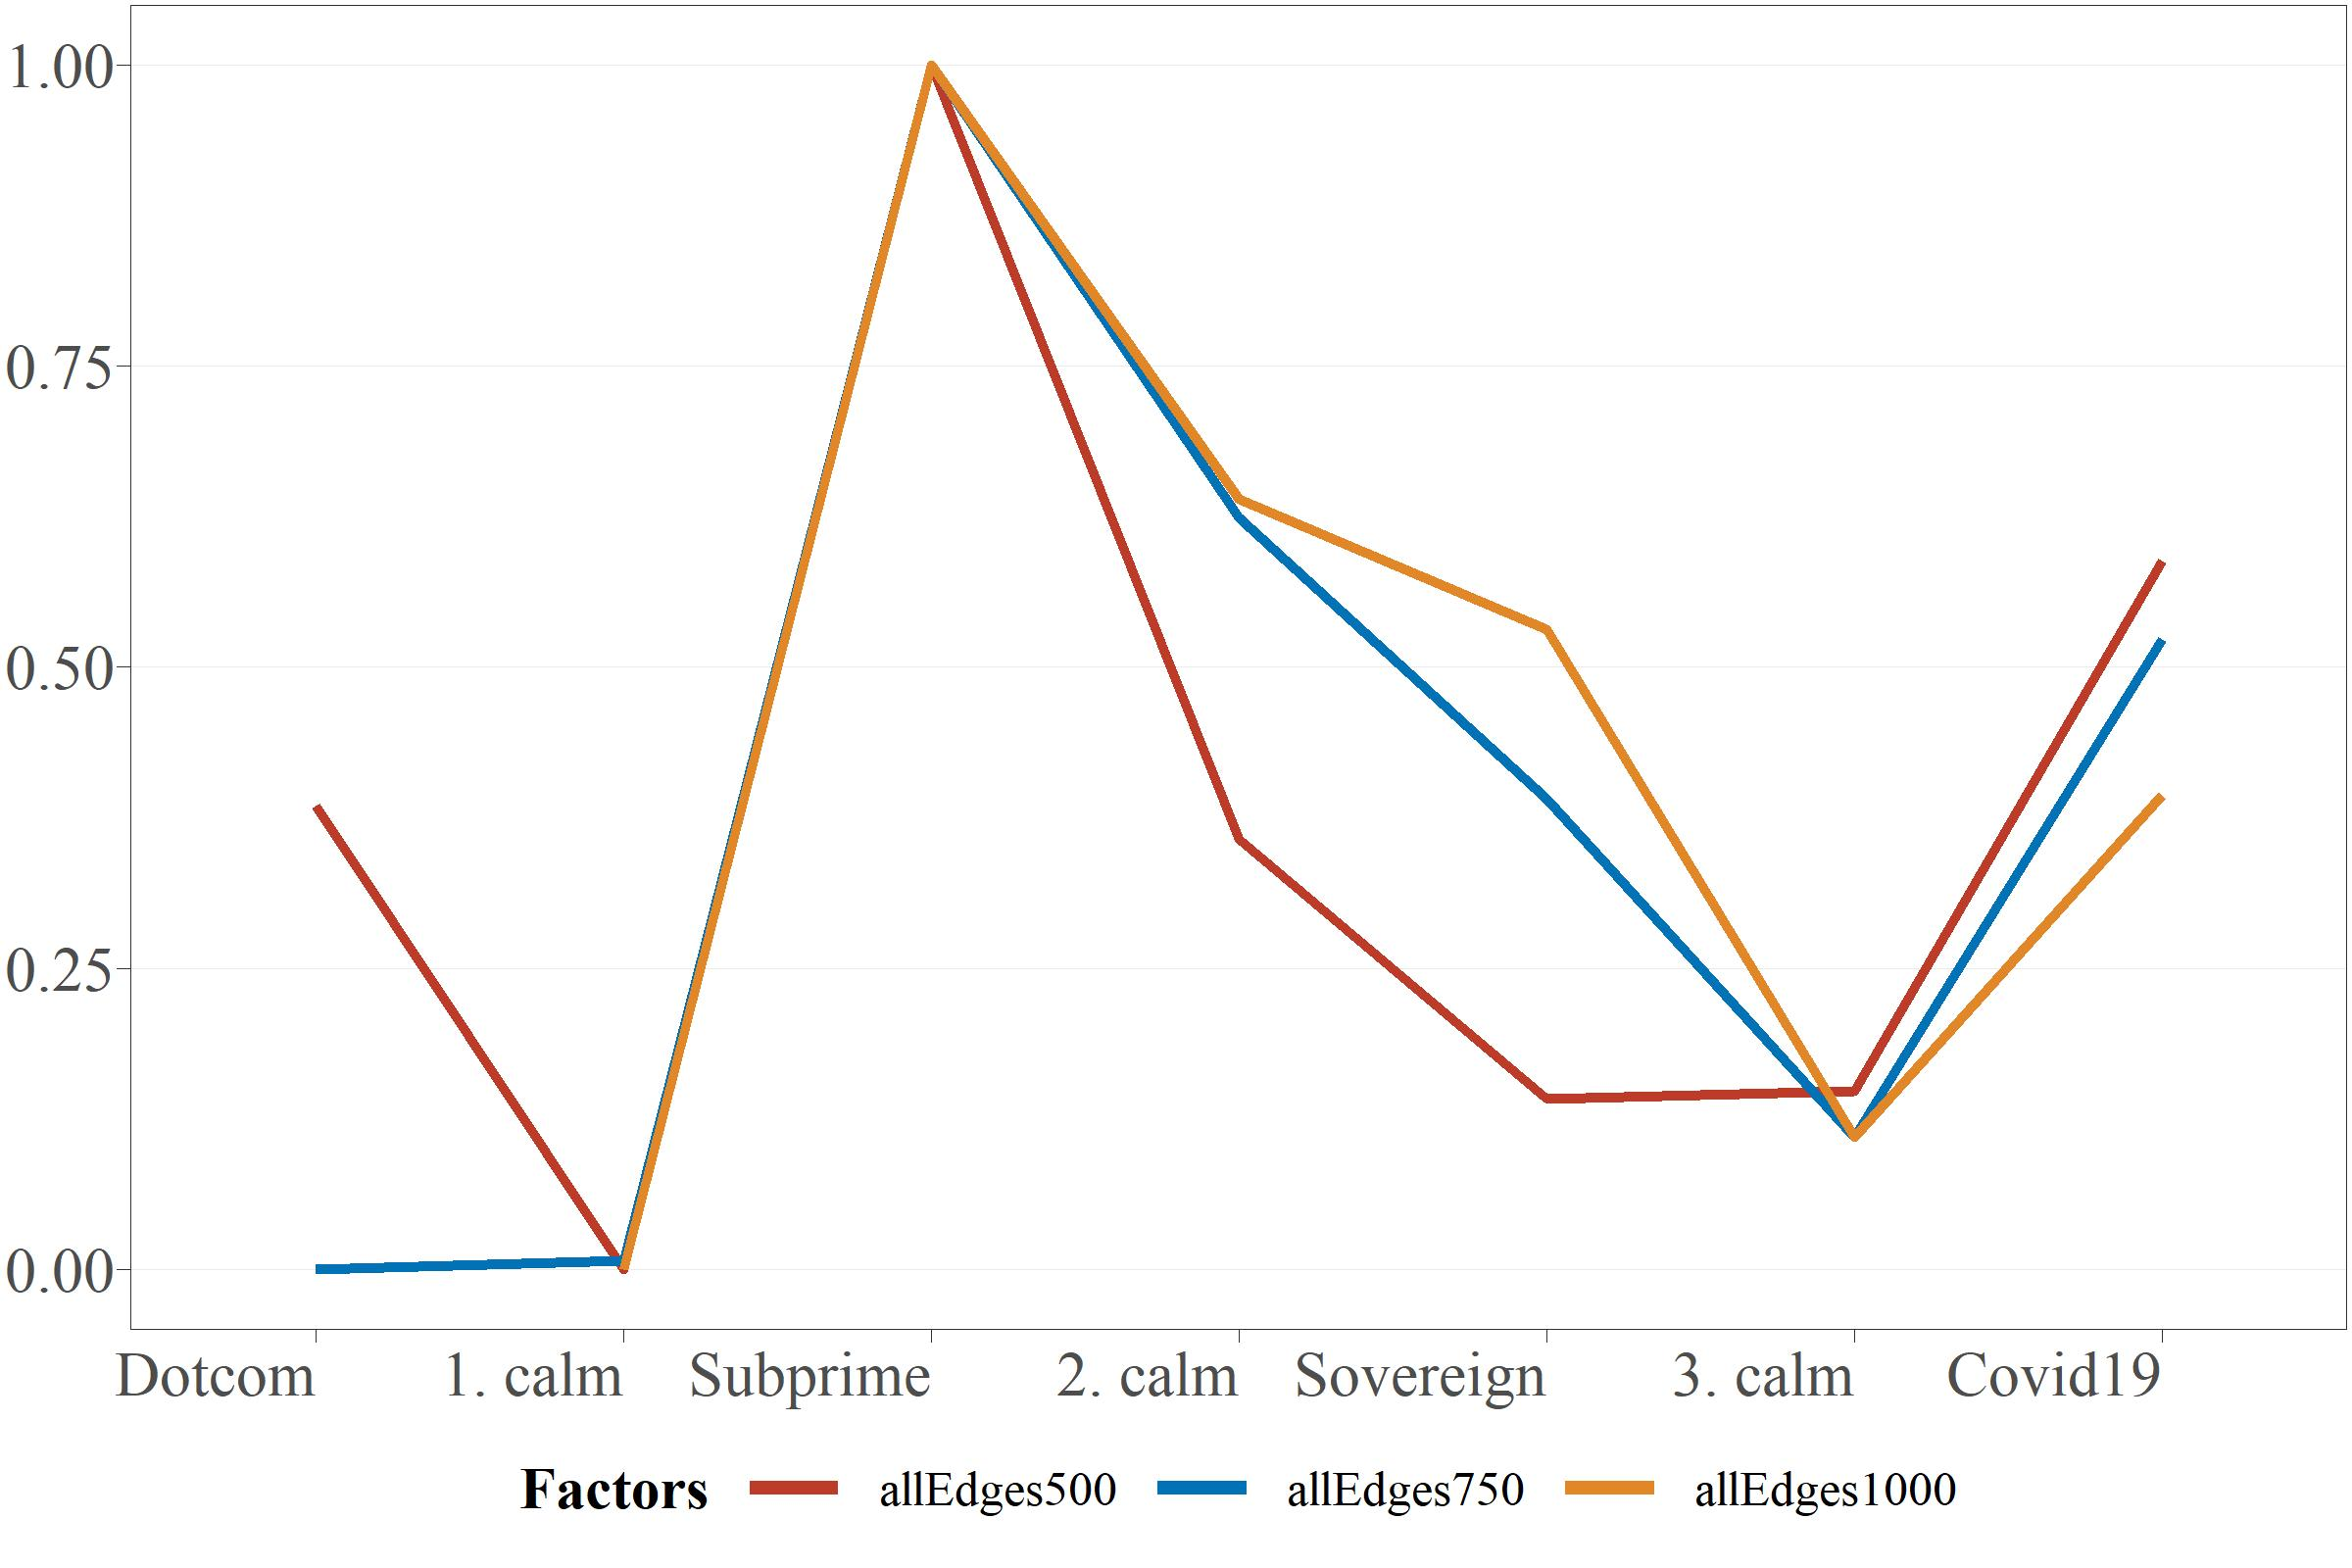
\includegraphics[width=13.5cm]{characteristics}
\centering

\caption{Summarized edge number by day, resulted by dynamic Toda-Yamamoto analysis }
\label{fig:differentWindowSizes}

\end{figure}

\subsection{Comparing Granger causality and Toda-Yamamoto causality}

In the interconnectedness related literature it is common to coroborate results with a Granger causality model. \cite{zhang2017oil} and \cite{umar2021oil} for example compared their results based on the Diebold-Yilmaz method to a Granger causality based approach. It is convinient for us as well since the Toda-Yamamoto framework is a modified Granger causality test. We run the two models with same parameters (lag selection is based on AIC and the window size is 750). The sum of edges for each day is shown on Figure \ref{fig:grangerVsTY}

\begin{figure}[H]
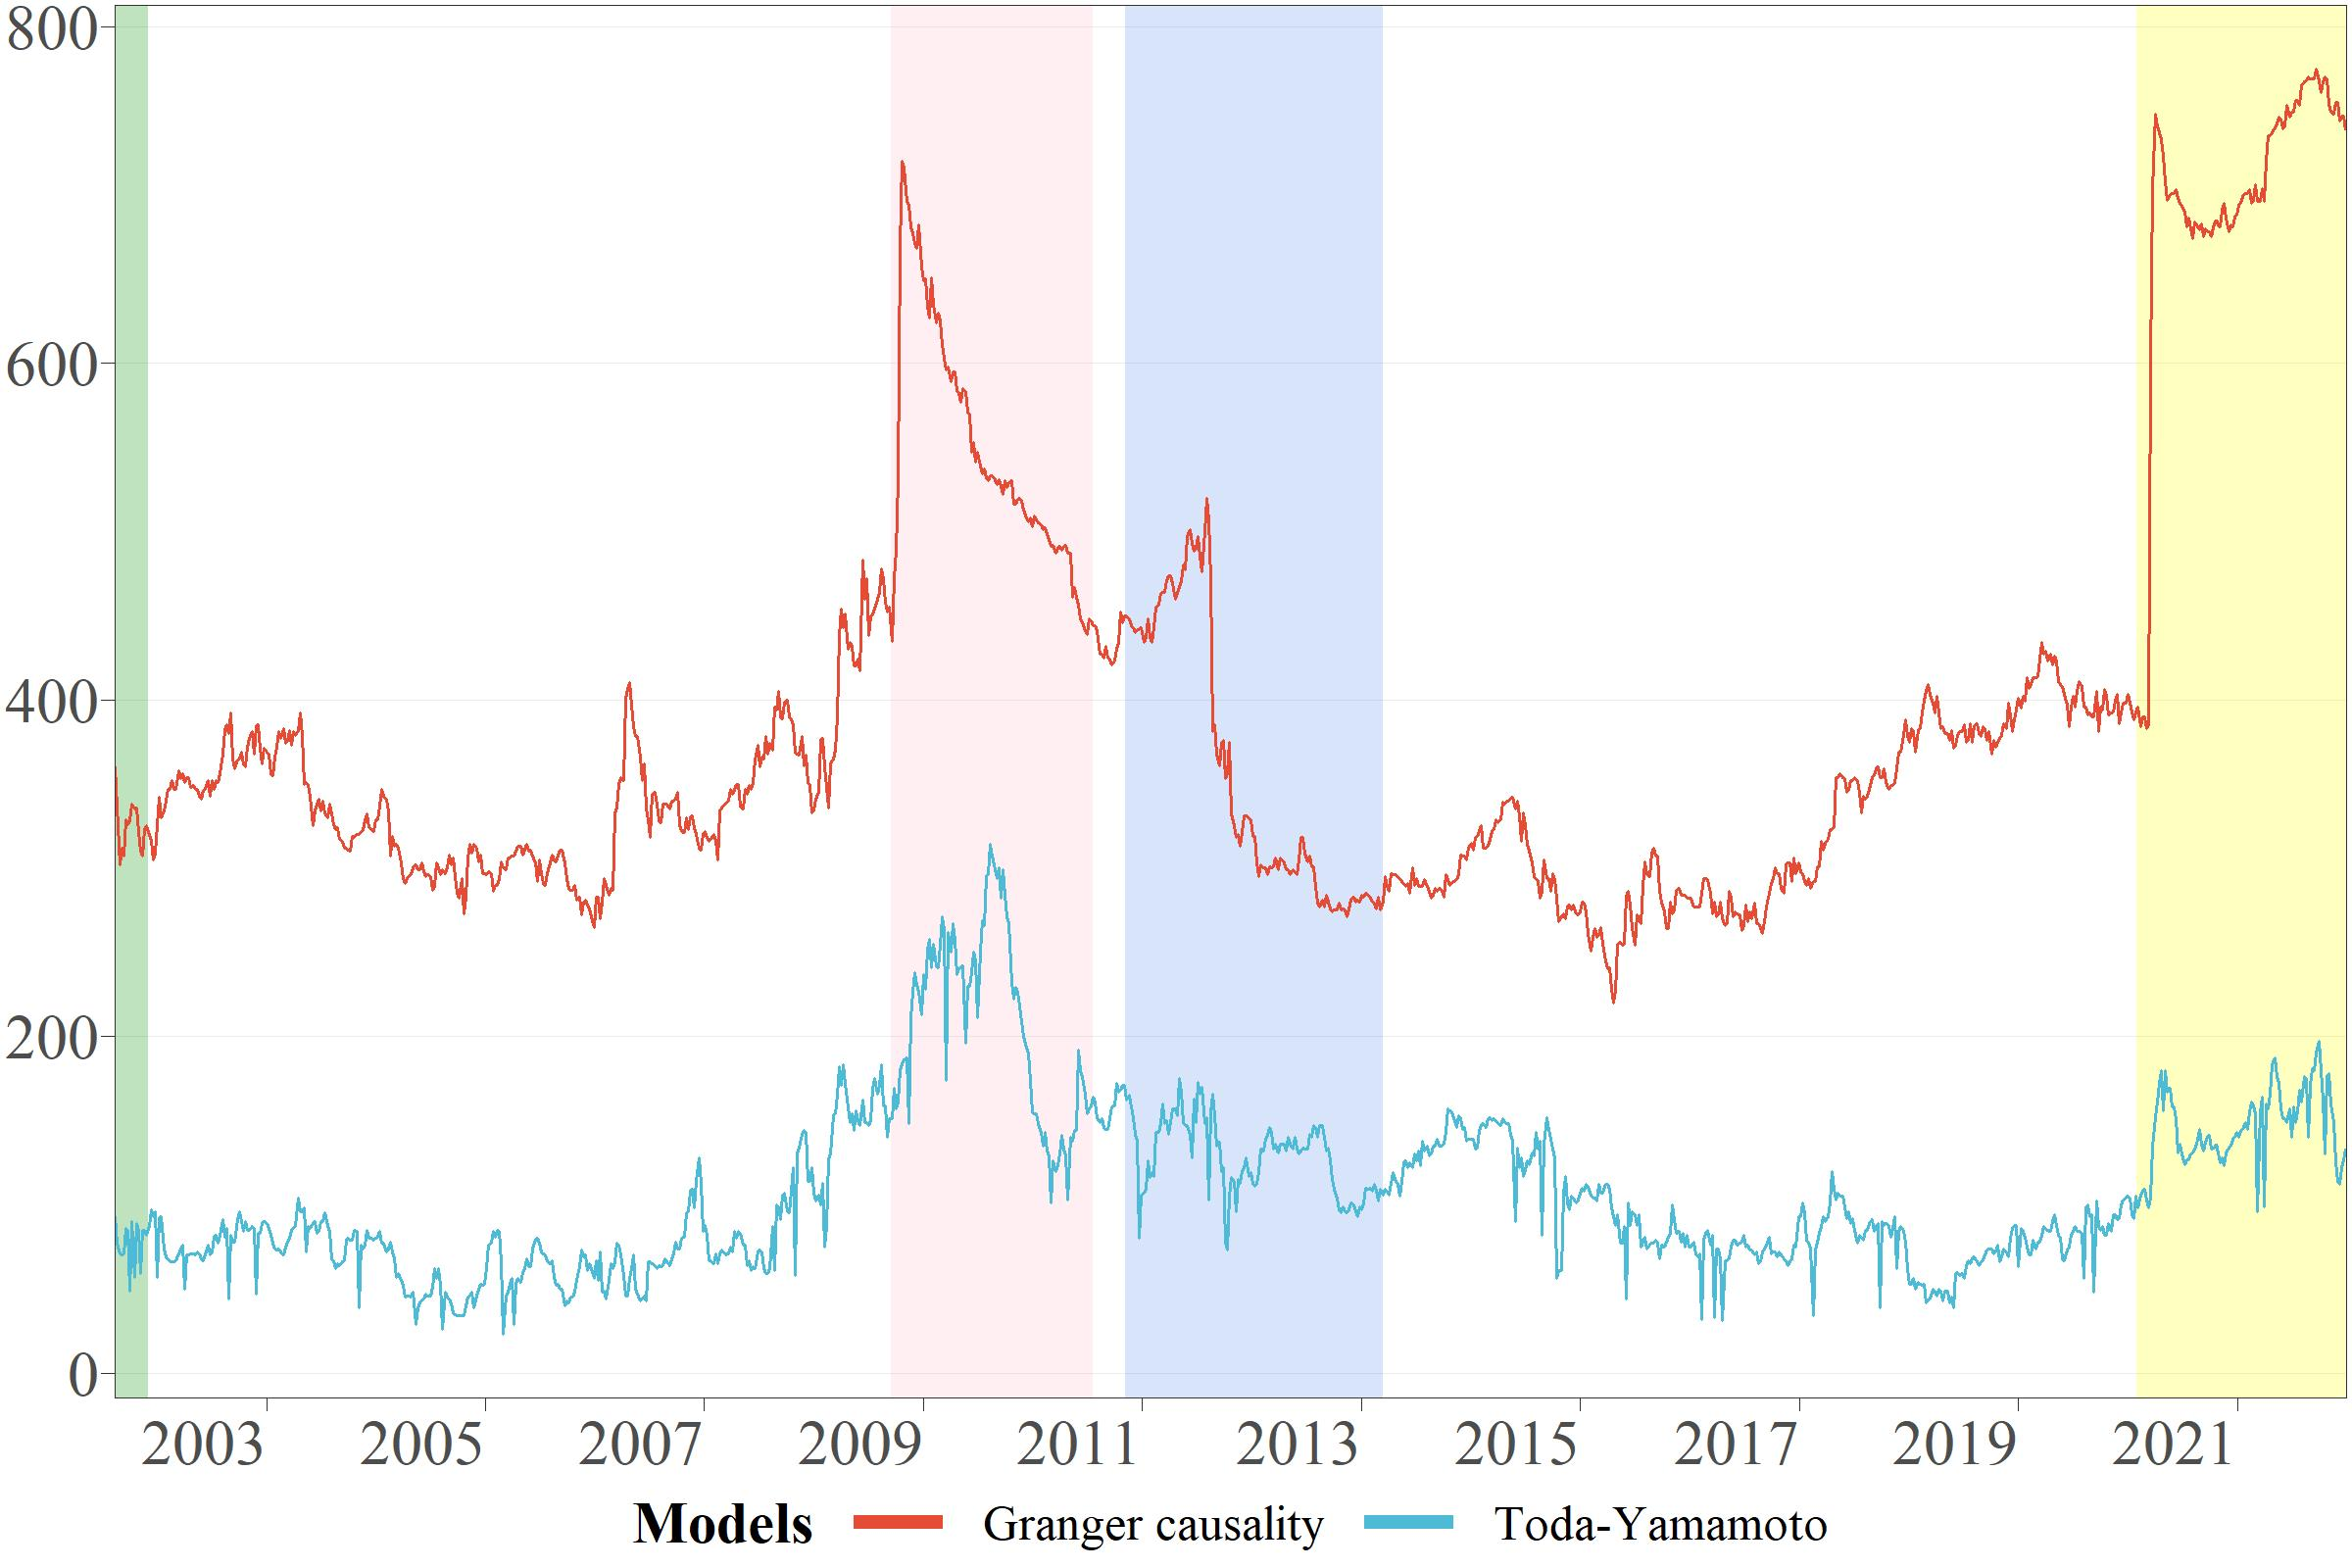
\includegraphics[width=13.5cm]{grangerVSty}
\centering

\caption{Summarized edge number by day, resulted by dynamic Toda-Yamamoto analysis }
\label{fig:grangerVsTY}
\centering
\fnote{
Widnow size: 750, Lag: based on AIC
}
\end{figure}

\section{Concluding remarks}


This paper determines the magnitude and direction of causality relationships in the maturity structure of interest rates of 12 developed countries.
The sovereign yield curves are modeled using the dynamic Nelson Siegel model by substracting the Level, Slope and Curvature factors which represent long, short and medium term interest rates.
The causality pairwise relationships are identified by the Toda-Yamamoto framework.

The results show that Slope factors have the highest number of causality effect followed by Level and Curvature. The dominant participant of the network is without doubt the USA, all three factors is net provider (the outgoing - incoming edge count is positive). The dynamics of the connectedness measure is captured by a rolling window technique. This indicates that edge number is increased durnig the turbulent periods. It is also reveiled that the USA is acting as net causality provider in all periods of the observed time frame, while stronger economies like Germany and Switzerland act as drivers of the univcerse durnig crises.

The results offer insights for policy makers on efficient monetary and macroeconomic policy
formulation. The co-movements of these factors are crucial for monetary authorities to
understand the impact of changes in short-term rates on long-term rates because these rates
determine borrowing costs and thereby aggregate demand in the economy (Wu, 2003). It also
helps global investors to understand the vulnerability of investing in these countries during times
of global turmoil and for efficient portfolio diversification.


%jpeg(paste0('C:\\Research\\Sovereign_interconnectedness\\Refactored\\plots\\factorTS\\',sheetName,'.jpeg'), width = 2400, height = 1600)
%ggplot() +
%geom_line(data=meltedLevels, aes(Period, value, color = `Factors`, size = `Factors`,group =Factors ),size=1.2)+
%scale_x_discrete(limits = c("Dotcom","1. calm","Subprime","2. calm","Sovereign","3. calm","Covid19"))+
%guides(colour = guide_legend(override.aes = list(size=5)))+
%  scale_size_manual(values = c(rep(1,20)))+
%  scale_color_nejm()+
%  scale_y_continuous() +
%  #scale_x_date(expand=c(0,0),date_breaks = "2 years",date_labels = "%Y")+
%  labs(x=NULL, y=NULL) +
%  theme_bw() +
%  theme(axis.text.x=element_text(hjust=1, vjust=0.5)) +
%  theme(text = element_text(size=80, family="serif"))+
%  theme(panel.grid.minor=element_blank()) +
%  theme(panel.grid.major.x=element_blank()) +
%  theme(plot.title = element_text(hjust = 0.5))+
%  theme(axis.ticks.length=unit(.5, "cm"))+
%  theme(legend.position = 'bottom',
%        legend.key.size = unit(3, "cm"),
%        legend.key.height = unit(5, 'cm'),
%        legend.key.width= unit(4, 'cm'),
%        legend.text = element_text(size =  50,  family="serif"),
%        legend.title = element_text(size = 60,  family="serif", face = "bold"))
%
%dev.off()



\bibliographystyle{te}


\bibliography{research}

\begin{appendices}



\begin{table}[H]

\fontsize{10}{10}\selectfont
\centering % used for centering table
\begin{tabular}{l c c c c c c}% centered columns (4 columns)
\hline\hline   \\ [-1.5ex]               %inserts double horizontal lines
%Case & Method\#1 & Method\#2 & Method\#3 & test \\  [0.5ex]
Node & Average & St. dev & Minimum & Maximum & \textrho(1)  & \textrho(10) \\ [0.5ex] % inserts table %heading

\hline       \\ [-1.5ex]           % inserts single horizontal line
\textit{\textbf{Australia}}	&		&		&		&		&		&		\\
1 year	&	3.65	&	1.94	&	-0.05	&	7.39	&	0.999	&	0.994	\\
5 years	&	4.02	&	1.90	&	0.24	&	7.30	&	0.999	&	0.994	\\
10 years	&	4.36	&	1.74	&	0.61	&	7.43	&	0.999	&	0.993	\\
30 years	&	4.78	&	1.46	&	1.17	&	7.67	&	0.999	&	0.099	\\
\textit{\textbf{Canada}}	&		&		&		&		&		&		\\
1 year	&	2.21	&	1.67	&	0.12	&	6.43	&	0.999	&	0.994	\\
5 years	&	2.87	&	1.68	&	0.28	&	6.70	&	0.999	&	0.994	\\
10 years	&	3.38	&	1.62	&	0.45	&	6.78	&	0.999	&	0.994	\\
30 years	&	3.64	&	1.42	&	0.71	&	6.25	&	0.999	&	0.994	\\
\textit{\textbf{Switzerland}}	&		&		&		&		&		&		\\
1 year	&	0.54	&	1.28	&	-1.09	&	3.83	&	0.999	&	0.994	\\
5 years	&	1.04	&	1.41	&	-1.11	&	3.97	&	1.000	&	0.996	\\
10 years	&	1.55	&	1.43	&	-0.97	&	4.20	&	1.000	&	0.995	\\
30 years	&	2.07	&	1.56	&	-0.70	&	4.95	&	1.000	&	0.994	\\
\textit{\textbf{Germany}}	&		&		&		&		&		&		\\
1 year	&	1.37	&	1.87	&	-0.99	&	5.24	&	1.000	&	0.996	\\
5 years	&	1.93	&	1.97	&	-1.01	&	5.39	&	0.999	&	0.996	\\
10 years	&	2.52	&	1.92	&	-0.87	&	5.75	&	1.000	&	0.996	\\
30 years	&	3.16	&	1.88	&	-0.47	&	6.48	&	1.000	&	0.994	\\
\textit{\textbf{Spain}}	&		&		&		&		&		&		\\
1 year	&	1.80	&	1.77	&	-0.80	&	6.44	&	1.000	&	0.990	\\
5 years	&	2.75	&	1.85	&	-0.45	&	7.65	&	0.999	&	0.992	\\
10 years	&	3.54	&	1.80	&	-0.01	&	7.67	&	0.999	&	0.992	\\
30 years	&	4.37	&	1.57	&	0.85	&	7.85	&	0.999	&	0.990	\\
\textit{\textbf{France}}	&		&		&		&		&		&		\\
1 year	&	1.42	&	1.84	&	-0.87	&	5.30	&	0.999	&	0.996	\\
5 years	&	2.11	&	1.88	&	-0.78	&	5.40	&	0.999	&	0.995	\\
10 years	&	2.82	&	1.84	&	-0.44	&	5.92	&	1.000	&	0.995	\\
30 years	&	3.57	&	1.66	&	0.24	&	6.51	&	1.000	&	0.993	\\
\textit{\textbf{Great Britain}}	&		&		&		&		&		&		\\
1 year	&	2.32	&	2.25	&	-0.17	&	6.62	&	1.000	&	0.995	\\
5 years	&	2.84	&	1.97	&	-0.11	&	6.52	&	0.999	&	0.995	\\
10 years	&	3.25	&	1.67	&	0.11	&	5.92	&	1.000	&	0.994	\\
30 years	&	3.47	&	1.26	&	0.53	&	5.06	&	1.000	&	0.991	\\
\textit{\textbf{Italy}}	&		&		&		&		&		&		\\
1 year	&	1.88	&	1.70	&	-0.59	&	8.17	&	0.999	&	0.989	\\
5 years	&	2.93	&	1.65	&	-0.10	&	7.76	&	0.999	&	0.989	\\
10 years	&	3.76	&	1.52	&	0.49	&	7.35	&	0.999	&	0.990	\\
30 years	&	4.59	&	1.32	&	1.50	&	7.37	&	0.999	&	0.988	\\
\textit{\textbf{Japan}}	&		&		&		&		&		&		\\
1 year	&	0.08	&	0.24	&	-0.35	&	0.84	&	0.999	&	0.989	\\
5 years	&	0.43	&	0.48	&	-0.39	&	1.72	&	0.999	&	0.987	\\
10 years	&	0.97	&	0.70	&	-0.28	&	2.58	&	0.999	&	0.991	\\
30 years	&	1.84	&	0.81	&	0.04	&	3.31	&	0.999	&	0.990\\
\textit{\textbf{South Korea}}	&		&		&		&		&		&		\\
1 year	&	3.18	&	2.28	&	0.35	&	13.51	&	0.999	&	0.978	\\
5 years	&	4.30	&	2.22	&	0.79	&	14.34	&	0.999	&	0.976	\\
10 years	&	5.05	&	2.11	&	1.44	&	15.12	&	0.996	&	0.972	\\
30 years	&	6.06	&	3.01	&	1.71	&	18.56	&	0.996	&	0.976	\\
\textit{\textbf{The Netherlands}}	&		&		&		&		&		&		\\
1 year	&	1.41	&	1.87	&	-0.94	&	5.31	&	0.995	&	0.996	\\
5 years	&	2.07	&	1.95	&	-0.85	&	5.52	&	0.996	&	0.996	\\
10 years	&	2.71	&	1.92	&	-0.63	&	5.91	&	1.000	&	0.995	\\
30 years	&	3.21	&	1.87	&	-0.39	&	7.56	&	1.000	&	0.994	\\
\textit{\textbf{USA}}	&		&		&		&		&		&		\\
1 year	&	1.95	&	1.94	&	0.04	&	7.07	&	1.000	&	0.996	\\
5 years	&	2.79	&	1.63	&	0.20	&	6.95	&	0.999	&	0.993	\\
10 years	&	3.46	&	1.44	&	0.50	&	6.92	&	0.999	&	0.991	\\
30 years	&	4.10	&	1.23	&	1.08	&	6.67	&	0.999	&	0.988	\\



\hline%inserts single line
\end{tabular}
\caption{Descriptive statistics of country yield curve nodes}% title of Table
\label{tab:curveDescripticeStatistics}
\end{table}
%----------------------------------------------------------------------------------------------------------------------------------------------------

\begin{table}[H]

\fontsize{10}{10}\selectfont
\centering% centering table
\captionsetup{justification=centering}

%------------------------------------------------ ADF table----------------------------------------------------------------------------
\begin{subtable}[t]{1\textwidth}
\centering% centering table
\begin{tabular}{l cc cc cc cc cc cc}
\hline\hline \\ [-1.5ex]                         
 

Country	&	\multicolumn{2}{c}{AUS}			&	\multicolumn{2}{c}{CAN}			&	\multicolumn{2}{c}{CHE}			&	\multicolumn{2}{c}{DEU}			&	\multicolumn{2}{c}{ESP}			&	\multicolumn{2}{c}{FRA}			\\[0.5ex] 

& value &P 		& value &P 			& value &P  		& value& P         			& value &P				& value &P\\

\hline       \\ [-1.5ex] 

Level		&	-3.84 & 0.02 		& -3.52 & 0.04 		& -3.16 & 0.10 		& -3.06 & 0.13 		& -1.63 & 0.74 		& -2.94 & 0.18	\\
Slope		&	-2.81 & 0.24 		& -2.06 & 0.55 		& -2.91 & 0.19 		& -2.37 & 0.42 		& -2.12 & 0.53 		& -2.21 & 0.49	\\
Curvature	&	-4.08 & 0.01 		& -3.01 & 0.15 		& -3.26 & 0.08 		& -3.05 & 0.13  		& -3.80 & 0.02 		& -2.97 & 0.17\\

\hline   \\ [-1.5ex]    

Country	&	\multicolumn{2}{c}{GBR}			&	\multicolumn{2}{c}{ITA}			&	\multicolumn{2}{c}{JPN}			&	\multicolumn{2}{c}{KOR}			&	\multicolumn{2}{c}{NLD}			&	\multicolumn{2}{c}{USA}			\\

 & value &P & value &P& value &P & value &P& value &P & value &P\\

\hline       \\ [-1.5ex] 

Level		&	-2.25 & 0.47 		& -1.91 & 0.61 		& -3.91 & 0.01 		& -5.61 & 0.01 		& -3.06 & 0.13 		& -4.71 & 0.01	\\
Slope		&	-1.84 & 0.64		& -2.70 & 0.28		& -4.98 & 0.01 		& -2.88 & 0.20 		& -2.20 & 0.49 		& -2.06 & 0.55	\\
Curvature	&	-1.84 & 0.65 		& -4.16 & 0.01 		& -3.49 & 0.04 		& -3.19 & 0.09 		& -3.38 & 0.06 		& -2.06 & 0.55\\
\hline
\end{tabular}
\caption{\textbf{ADF test results}}
\end{subtable}
\hspace{\fill}
%----------------------------------------------------------------------------------------------------------------------------------------------------
\bigskip 

%------------------------------------------------ KPSS table----------------------------------------------------------------------------
\begin{subtable}[t]{1\textwidth}
\centering% centering table
\begin{tabular}{l cc cc cc cc cc cc}% creating eight columns
\hline\hline \\ [-1.5ex]                         %inserting double-line
%Audio Name&\multicolumn{2}{c}{Sum of Extracted Bits}&\multicolumn{4}{c}{Sum of Extracted Bits} \\ [0.5ex] 

Country	&	\multicolumn{2}{c}{AUS}			&	\multicolumn{2}{c}{CAN}			&	\multicolumn{2}{c}{CHE}			&	\multicolumn{2}{c}{DEU}			&	\multicolumn{2}{c}{ESP}			&	\multicolumn{2}{c}{FRA}			\\[0.5ex] 

 & value &P & value &P& value &P & value &P& value &P & value &P\\

\hline       \\ [-1.5ex] 

Level	&	42.25 & 0.01 		& 47.24 & 0.01 		& 47.59 & 0.01 		& 47.03 & 0.01 		& 26.92 & 0.01 		& 44.16 & 0.01	\\
Slope	&	2.58 & 0.01 		& 5.55 & 0.01 		& 18.27 & 0.01 		& 6.84 & 0.01 		& 5.38 & 0.01 		& 4.24 & 0.01	\\
Curvature	&25.23 & 0.01 	& 9.07 & 0.01 		& 2.50 & 0.01 		& 4.45 & 0.01 		& 13.02 & 0.01 		& 9.08 & 0.01	\\


\hline   \\ [-1.5ex]    

Country	&	\multicolumn{2}{c}{GBR}			&	\multicolumn{2}{c}{ITA}			&	\multicolumn{2}{c}{JPN}			&	\multicolumn{2}{c}{KOR}			&	\multicolumn{2}{c}{NLD}			&	\multicolumn{2}{c}{USA}			\\

 & value &P & value &P& value &P & value &P& value &P & value &P\\

\hline       \\ [-1.5ex] 

Level	&	37.28 & 0.01 		& 27.33 & 0.01 		& 40.71 & 0.01 		& 40.11 & 0.01 		& 46.48 & 0.01 		& 43.70 & 0.01	\\
Slope	&	12.42 & 0.01 		& 7.46 & 0.01 		& 42.11 & 0.01 		& 8.49 & 0.01 		& 5.97 & 0.01 		& 4.04 & 0.01	\\
Curvature	&24.43 & 0.01 	& 10.23 & 0.01 		& 22.73 & 0.01 		& 6.71 & 0.01 		& 4.04 & 0.01 		& 6.11 & 0.01	\\


\hline
\end{tabular}
\caption{\textbf{KPSS test results}}

\end{subtable}
\hspace{\fill}
%----------------------------------------------------------------------------------------------------------------------------------------------------
\bigskip

%------------------------------------------------ ADF(1) table----------------------------------------------------------------------------
\begin{subtable}[t]{1\textwidth}
\centering
\begin{tabular}{l cc cc cc cc cc cc}% creating eight columns
\hline\hline \\ [-1.5ex]                         %inserting double-line
%Audio Name&\multicolumn{2}{c}{Sum of Extracted Bits}&\multicolumn{4}{c}{Sum of Extracted Bits} \\ [0.5ex] 

Country	&	\multicolumn{2}{c}{AUS}			&	\multicolumn{2}{c}{CAN}			&	\multicolumn{2}{c}{CHE}			&	\multicolumn{2}{c}{DEU}			&	\multicolumn{2}{c}{ESP}			&	\multicolumn{2}{c}{FRA}			\\[0.5ex] 

 & value &P & value &P& value &P & value &P& value &P & value &P\\

\hline       \\ [-1.5ex] 

Level	&	-17.73 & 0.01 	& -17.65 & 0.01 		& -17.95 & 0.01 		& -18.79 & 0.01 		& -18.26 & 0.01 		& -17.29 & 0.01	\\
Slope	&	-16.75 & 0.01 	& -15.80 & 0.01 		& -17.44 & 0.01 		& -17.42 & 0.01 		& -17.68 & 0.01 		& -16.12 & 0.01	\\
Curvature	& -4.10 & 0.01 	& -17.59 & 0.01 		& -17.68 & 0.01 		& -18.45 & 0.01 		& -18.55 & 0.01 		& -18.34 & 0.01	\\


\hline   \\ [-1.5ex]    

Country	&	\multicolumn{2}{c}{GBR}			&	\multicolumn{2}{c}{ITA}			&	\multicolumn{2}{c}{JPN}			&	\multicolumn{2}{c}{KOR}			&	\multicolumn{2}{c}{NLD}			&	\multicolumn{2}{c}{USA}			\\

 & value &P & value &P& value &P & value &P& value &P & value &P\\

\hline       \\ [-1.5ex] 

Level	&	-18.08 & 0.01 		& -18.30 & 0.01 		& -17.39 & 0.01 		& -5.22 & 0.01 		& -18.56 & 0.01 		& -4.70 & 0.01	\\
Slope	&		-16.09 & 0.01 	& -15.68 & 0.01 		& -4.93 & 0.01 		& -16.82 & 0.01 		& -16.75 & 0.01 		& -16.42 & 0.01	\\
Curvature	&	-17.91 & 0.01 	& -4.14 & 0.01 		& -18.07 & 0.01 		& -19.20 & 0.01 		& -18.86 & 0.01 		& -18.83 & 0.01	\\



\hline
\end{tabular}
\caption{\textbf{ADF(1) test results}}
\end{subtable}
\hspace{\fill}
%----------------------------------------------------------------------------------------------------------------------------------------------------
\bigskip 

%------------------------------------------------ KPS (1) table----------------------------------------------------------------------------
\begin{subtable}[t]{1\textwidth}
\centering
\begin{tabular}{l cc cc cc cc cc cc}% creating eight columns
\hline\hline \\ [-1.5ex]                         %inserting double-line
%Audio Name&\multicolumn{2}{c}{Sum of Extracted Bits}&\multicolumn{4}{c}{Sum of Extracted Bits} \\ [0.5ex] 

Country	&	\multicolumn{2}{c}{AUS}			&	\multicolumn{2}{c}{CAN}			&	\multicolumn{2}{c}{CHE}			&	\multicolumn{2}{c}{DEU}			&	\multicolumn{2}{c}{ESP}			&	\multicolumn{2}{c}{FRA}			\\[0.5ex] 

 & value &P & value &P& value &P & value &P& value &P & value &P\\

\hline       \\ [-1.5ex] 

Level	&	0.06 & 0.1 		& 0.05 & 0.1 		& 0.03 & 0.1 		& 0.08 & 0.1 		& 0.12 & 0.1 		& 0.09 & 0.1	\\
Slope	&	0.04 & 0.1 		& 0.18 & 0.1 		& 0.03 & 0.1 		& 0.08 & 0.1 		& 0.09 & 0.1 		& 0.09 & 0.1\\
Curvature&	0.03& 0.1 		& 0.05 & 0.1 		& 0.06 & 0.1 		& 0.04 & 0.1 		& 0.03 & 0.1 		& 0.03 & 0.1\\


\hline   \\ [-1.5ex]    

Country	&	\multicolumn{2}{c}{GBR}			&	\multicolumn{2}{c}{ITA}			&	\multicolumn{2}{c}{JPN}			&	\multicolumn{2}{c}{KOR}			&	\multicolumn{2}{c}{NLD}			&	\multicolumn{2}{c}{USA}			\\

 & value &P & value &P& value &P & value &P& value &P & value &P\\

\hline       \\ [-1.5ex] 

Level	&	0.09 & 0.1 		& 0.11 & 0.1 		& 0.15 & 0.1 		& 0.21 & 0.1 		& 0.09 & 0.1 		& 0.05 & 0.1	\\
Slope	&	0.32 & 0.1 		& 0.10 & 0.1 		& 0.09 & 0.1 		& 0.04 & 0.1 		& 0.09 & 0.1 		& 0.15 & 0.1 \\
Curvature	&0.10 & 0.1 		& 0.02 & 0.1 		& 0.12 & 0.1 		& 0.02 & 0.1 		& 0.03 & 0.1 		& 0.06 & 0.1	\\


\hline
\end{tabular}
\caption{\textbf{KPSS(1) test results}}
\end{subtable}
\hspace{\fill}
%----------------------------------------------------------------------------------------------------------------------------------------------------
%\label{tab:table1}
\caption{Results of unit-root tests}
\label{tab:unitRootTest}
\end{table}

%----------------------------------------------------------------------------------------------------------------------------------------------------


\begin{table}[H]
\fontsize{10}{10}\selectfont
\centering% centering table
\begin{tabular}{l  cccccccc}% creating eight columns
\hline\hline \\ [-1.5ex]                         %inserting double-line


				& Whole period  &Dotcom	&1. calm  & Subprime & 2. calm &Sovereign & 3. calm & Covid19 \\
\hline \\ [-1.5ex]  
Level	&	3.2	&	0.3	&	1.9	&	7.9	&	3.8	&	4.7	&	2.2	&	5.0	\\
Slope	&	4.1	&	2.7	&	2.0	&	8.6	&	4.5	&	6.9	&	3.8	&	5.0	\\
Curvature	&	3.6	&	2.2	&	2.5	&	5.7	&	4.6	&	3.9	&	3.5	&	5.8	\\
Cross connections	&	27.0	&	8.0	&	16.7	&	50.0	&	34.9	&	40.3	&	23.8	&	38.4	\\
All edges	&	37.9	&	13.2	&	23.1	&	72.1	&	47.9	&	55.8	&	33.3	&	54.2	\\


%----------------------------------------------------------------------------------------------------------------------------------------------------

\hline            
\end{tabular}
\caption{Average edge count by edges during the seven sub-periods - 750 observations long window size} %title of the table
\label{tab:euroEdges}
\end{table}











%----------------------------------------------------------------------------------------------------------------------------------------------------
\addtolength{\tabcolsep}{-1pt}   
\begin{table}[H]

\fontsize{10}{10}\selectfont
\centering% centering table
\begin{tabular}{l  cccccccc@{\hskip 0.2in}  cccccccc@{\hskip 0.2in}   ccccccc}% creating eight columns

\hline\hline \\ [-1.5ex]                         %inserting double-line

\multicolumn{1}{c}{}&\multicolumn{8}{c}{500}			&	\multicolumn{8}{c}{750} &	\multicolumn{7}{c}{1000}	\\	
\hline \\ [-1.5ex]    
& \rot{Whole period}  &\rot{Dotcom}	&\rot{1. calm}  & \rot{Subprime} & \rot{2. calm} & \rot{Sovereign} & \rot{3. calm} & \rot{Covid19} & \rot{Whole period}  &\rot{Dotcom}	&\rot{1. calm}  & \rot{Subprime} & \rot{2. calm} & \rot{Sovereign} & \rot{3. calm} & \rot{Covid19} & \rot{Whole period}  &\rot{1. calm}  & \rot{Subprime} & \rot{2. calm} & \rot{Sovereign} & \rot{3. calm} & \rot{Covid19} \\

\hline \\ [-1.5ex]    

AUS L	&\cellcolor{red!25}-	&\cellcolor{red!25}-	&\cellcolor{red!25}-	&\cellcolor{red!25}-	&\cellcolor{red!25}-	&\cellcolor{red!25}-	&\cellcolor{green!25}+	&\cellcolor{red!25}-	&\cellcolor{red!25}-	&\cellcolor{red!25}-	&\cellcolor{red!25}-	&\cellcolor{red!25}-	&\cellcolor{red!25}-	&\cellcolor{red!25}-	&\cellcolor{red!25}-	&\cellcolor{red!25}-	&\cellcolor{red!25}-	&\cellcolor{red!25}-	&\cellcolor{red!25}-	&\cellcolor{red!25}-	&\cellcolor{green!25}+	&\cellcolor{green!25}+	&\cellcolor{red!25}-\\
CAN L	&\cellcolor{green!25}+	&\cellcolor{green!25}+	&\cellcolor{green!25}+	&\cellcolor{green!25}+	&\cellcolor{yellow!25}0	&\cellcolor{green!25}+	&\cellcolor{green!25}+	&\cellcolor{green!25}+	&\cellcolor{green!25}+	&\cellcolor{green!25}+	&\cellcolor{green!25}+	&\cellcolor{red!25}-	&\cellcolor{red!25}-	&\cellcolor{green!25}+	&\cellcolor{green!25}+	&\cellcolor{green!25}+	&\cellcolor{green!25}+	&\cellcolor{green!25}+	&\cellcolor{green!25}+	&\cellcolor{green!25}+	&\cellcolor{red!25}-	&\cellcolor{green!25}+	&\cellcolor{green!25}+\\
CHE L	&\cellcolor{green!25}+	&\cellcolor{green!25}+	&\cellcolor{green!25}+	&\cellcolor{green!25}+	&\cellcolor{green!25}+	&\cellcolor{green!25}+	&\cellcolor{green!25}+	&\cellcolor{green!25}+	&\cellcolor{green!25}+	&\cellcolor{green!25}+	&\cellcolor{green!25}+	&\cellcolor{green!25}+	&\cellcolor{green!25}+	&\cellcolor{green!25}+	&\cellcolor{green!25}+	&\cellcolor{green!25}+	&\cellcolor{green!25}+	&\cellcolor{green!25}+	&\cellcolor{green!25}+	&\cellcolor{green!25}+	&\cellcolor{green!25}+	&\cellcolor{green!25}+	&\cellcolor{green!25}+\\
DEU L	&\cellcolor{green!25}+	&\cellcolor{red!25}-	&\cellcolor{green!25}+	&\cellcolor{red!25}-	&\cellcolor{red!25}-	&\cellcolor{green!25}+	&\cellcolor{green!25}+	&\cellcolor{red!25}-	&\cellcolor{green!25}+	&\cellcolor{red!25}-	&\cellcolor{green!25}+	&\cellcolor{green!25}+	&\cellcolor{green!25}+	&\cellcolor{green!25}+	&\cellcolor{red!25}-	&\cellcolor{green!25}+	&\cellcolor{green!25}+	&\cellcolor{green!25}+	&\cellcolor{green!25}+	&\cellcolor{green!25}+	&\cellcolor{green!25}+	&\cellcolor{red!25}-	&\cellcolor{red!25}-\\
ESP L	&\cellcolor{green!25}+	&\cellcolor{red!25}-	&\cellcolor{red!25}-	&\cellcolor{green!25}+	&\cellcolor{red!25}-	&\cellcolor{red!25}-	&\cellcolor{green!25}+	&\cellcolor{green!25}+	&\cellcolor{green!25}+	&\cellcolor{red!25}-	&\cellcolor{red!25}-	&\cellcolor{green!25}+	&\cellcolor{green!25}+	&\cellcolor{red!25}-	&\cellcolor{green!25}+	&\cellcolor{green!25}+	&\cellcolor{green!25}+	&\cellcolor{red!25}-	&\cellcolor{green!25}+	&\cellcolor{red!25}-	&\cellcolor{green!25}+	&\cellcolor{red!25}-	&\cellcolor{green!25}+\\
FRA L	&\cellcolor{red!25}-	&\cellcolor{red!25}-	&\cellcolor{red!25}-	&\cellcolor{red!25}-	&\cellcolor{green!25}+	&\cellcolor{red!25}-	&\cellcolor{green!25}+	&\cellcolor{red!25}-	&\cellcolor{red!25}-	&\cellcolor{red!25}-	&\cellcolor{green!25}+	&\cellcolor{red!25}-	&\cellcolor{red!25}-	&\cellcolor{red!25}-	&\cellcolor{green!25}+	&\cellcolor{red!25}-	&\cellcolor{green!25}+	&\cellcolor{green!25}+	&\cellcolor{red!25}-	&\cellcolor{red!25}-	&\cellcolor{red!25}-	&\cellcolor{green!25}+	&\cellcolor{green!25}+\\
GBR L	&\cellcolor{red!25}-	&\cellcolor{red!25}-	&\cellcolor{green!25}+	&\cellcolor{red!25}-	&\cellcolor{green!25}+	&\cellcolor{red!25}-	&\cellcolor{green!25}+	&\cellcolor{red!25}-	&\cellcolor{red!25}-	&\cellcolor{red!25}-	&\cellcolor{red!25}-	&\cellcolor{red!25}-	&\cellcolor{red!25}-	&\cellcolor{red!25}-	&\cellcolor{red!25}-	&\cellcolor{green!25}+	&\cellcolor{red!25}-	&\cellcolor{red!25}-	&\cellcolor{red!25}-	&\cellcolor{red!25}-	&\cellcolor{red!25}-	&\cellcolor{red!25}-	&\cellcolor{green!25}+\\
ITA L	&\cellcolor{green!25}+	&\cellcolor{green!25}+	&\cellcolor{red!25}-	&\cellcolor{red!25}-	&\cellcolor{green!25}+	&\cellcolor{red!25}-	&\cellcolor{red!25}-	&\cellcolor{green!25}+	&\cellcolor{green!25}+	&\cellcolor{green!25}+	&\cellcolor{green!25}+	&\cellcolor{green!25}+	&\cellcolor{red!25}-	&\cellcolor{red!25}-	&\cellcolor{yellow!25}0	&\cellcolor{green!25}+	&\cellcolor{red!25}-	&\cellcolor{green!25}+	&\cellcolor{green!25}+	&\cellcolor{green!25}+	&\cellcolor{red!25}-	&\cellcolor{red!25}-	&\cellcolor{green!25}+\\
JPN L	&\cellcolor{red!25}-	&\cellcolor{green!25}+	&\cellcolor{green!25}+	&\cellcolor{green!25}+	&\cellcolor{green!25}+	&\cellcolor{red!25}-	&\cellcolor{green!25}+	&\cellcolor{red!25}-	&\cellcolor{green!25}+	&\cellcolor{green!25}+	&\cellcolor{green!25}+	&\cellcolor{green!25}+	&\cellcolor{red!25}-	&\cellcolor{red!25}-	&\cellcolor{red!25}-	&\cellcolor{green!25}+	&\cellcolor{red!25}-	&\cellcolor{green!25}+	&\cellcolor{green!25}+	&\cellcolor{green!25}+	&\cellcolor{red!25}-	&\cellcolor{red!25}-	&\cellcolor{green!25}+\\
KOR L	&\cellcolor{green!25}+	&\cellcolor{green!25}+	&\cellcolor{red!25}-	&\cellcolor{green!25}+	&\cellcolor{green!25}+	&\cellcolor{red!25}-	&\cellcolor{green!25}+	&\cellcolor{green!25}+	&\cellcolor{green!25}+	&\cellcolor{green!25}+	&\cellcolor{green!25}+	&\cellcolor{green!25}+	&\cellcolor{red!25}-	&\cellcolor{green!25}+	&\cellcolor{green!25}+	&\cellcolor{green!25}+	&\cellcolor{green!25}+	&\cellcolor{green!25}+	&\cellcolor{red!25}-	&\cellcolor{green!25}+	&\cellcolor{green!25}+	&\cellcolor{green!25}+	&\cellcolor{green!25}+\\
NLD L	&\cellcolor{red!25}-	&\cellcolor{red!25}-	&\cellcolor{red!25}-	&\cellcolor{red!25}-	&\cellcolor{green!25}+	&\cellcolor{green!25}+	&\cellcolor{red!25}-	&\cellcolor{red!25}-	&\cellcolor{red!25}-	&\cellcolor{green!25}+	&\cellcolor{red!25}-	&\cellcolor{red!25}-	&\cellcolor{green!25}+	&\cellcolor{red!25}-	&\cellcolor{red!25}-	&\cellcolor{red!25}-	&\cellcolor{red!25}-	&\cellcolor{red!25}-	&\cellcolor{green!25}+	&\cellcolor{red!25}-	&\cellcolor{red!25}-	&\cellcolor{red!25}-	&\cellcolor{red!25}-\\
USA L	&\cellcolor{green!25}+	&\cellcolor{green!25}+	&\cellcolor{green!25}+	&\cellcolor{green!25}+	&\cellcolor{green!25}+	&\cellcolor{green!25}+	&\cellcolor{green!25}+	&\cellcolor{green!25}+	&\cellcolor{green!25}+	&\cellcolor{green!25}+	&\cellcolor{green!25}+	&\cellcolor{green!25}+	&\cellcolor{green!25}+	&\cellcolor{green!25}+	&\cellcolor{green!25}+	&\cellcolor{green!25}+	&\cellcolor{green!25}+	&\cellcolor{green!25}+	&\cellcolor{green!25}+	&\cellcolor{green!25}+	&\cellcolor{green!25}+	&\cellcolor{green!25}+	&\cellcolor{green!25}+\\
AUS S	&\cellcolor{red!25}-	&\cellcolor{red!25}-	&\cellcolor{red!25}-	&\cellcolor{green!25}+	&\cellcolor{green!25}+	&\cellcolor{red!25}-	&\cellcolor{red!25}-	&\cellcolor{red!25}-	&\cellcolor{red!25}-	&\cellcolor{red!25}-	&\cellcolor{red!25}-	&\cellcolor{green!25}+	&\cellcolor{red!25}-	&\cellcolor{red!25}-	&\cellcolor{red!25}-	&\cellcolor{red!25}-	&\cellcolor{red!25}-	&\cellcolor{red!25}-	&\cellcolor{green!25}+	&\cellcolor{red!25}-	&\cellcolor{red!25}-	&\cellcolor{red!25}-	&\cellcolor{red!25}-\\
CAN S	&\cellcolor{green!25}+	&\cellcolor{red!25}-	&\cellcolor{green!25}+	&\cellcolor{red!25}-	&\cellcolor{red!25}-	&\cellcolor{green!25}+	&\cellcolor{green!25}+	&\cellcolor{green!25}+	&\cellcolor{green!25}+	&\cellcolor{green!25}+	&\cellcolor{green!25}+	&\cellcolor{green!25}+	&\cellcolor{green!25}+	&\cellcolor{green!25}+	&\cellcolor{green!25}+	&\cellcolor{green!25}+	&\cellcolor{green!25}+	&\cellcolor{green!25}+	&\cellcolor{red!25}-	&\cellcolor{green!25}+	&\cellcolor{green!25}+	&\cellcolor{green!25}+	&\cellcolor{green!25}+\\
CHE S	&\cellcolor{green!25}+	&\cellcolor{green!25}+	&\cellcolor{green!25}+	&\cellcolor{red!25}-	&\cellcolor{red!25}-	&\cellcolor{green!25}+	&\cellcolor{red!25}-	&\cellcolor{green!25}+	&\cellcolor{green!25}+	&\cellcolor{green!25}+	&\cellcolor{green!25}+	&\cellcolor{red!25}-	&\cellcolor{red!25}-	&\cellcolor{red!25}-	&\cellcolor{red!25}-	&\cellcolor{green!25}+	&\cellcolor{red!25}-	&\cellcolor{green!25}+	&\cellcolor{red!25}-	&\cellcolor{red!25}-	&\cellcolor{red!25}-	&\cellcolor{green!25}+	&\cellcolor{red!25}-\\
DEU S	&\cellcolor{green!25}+	&\cellcolor{green!25}+	&\cellcolor{green!25}+	&\cellcolor{green!25}+	&\cellcolor{red!25}-	&\cellcolor{red!25}-	&\cellcolor{red!25}-	&\cellcolor{red!25}-	&\cellcolor{green!25}+	&\cellcolor{green!25}+	&\cellcolor{green!25}+	&\cellcolor{green!25}+	&\cellcolor{green!25}+	&\cellcolor{red!25}-	&\cellcolor{red!25}-	&\cellcolor{red!25}-	&\cellcolor{red!25}-	&\cellcolor{green!25}+	&\cellcolor{green!25}+	&\cellcolor{green!25}+	&\cellcolor{red!25}-	&\cellcolor{red!25}-	&\cellcolor{red!25}-\\
ESP S	&\cellcolor{red!25}-	&\cellcolor{red!25}-	&\cellcolor{red!25}-	&\cellcolor{red!25}-	&\cellcolor{red!25}-	&\cellcolor{red!25}-	&\cellcolor{red!25}-	&\cellcolor{green!25}+	&\cellcolor{red!25}-	&\cellcolor{red!25}-	&\cellcolor{red!25}-	&\cellcolor{green!25}+	&\cellcolor{green!25}+	&\cellcolor{green!25}+	&\cellcolor{red!25}-	&\cellcolor{green!25}+	&\cellcolor{red!25}-	&\cellcolor{red!25}-	&\cellcolor{red!25}-	&\cellcolor{red!25}-	&\cellcolor{red!25}-	&\cellcolor{green!25}+	&\cellcolor{green!25}+\\
FRA S	&\cellcolor{red!25}-	&\cellcolor{red!25}-	&\cellcolor{red!25}-	&\cellcolor{red!25}-	&\cellcolor{red!25}-	&\cellcolor{red!25}-	&\cellcolor{red!25}-	&\cellcolor{red!25}-	&\cellcolor{red!25}-	&\cellcolor{red!25}-	&\cellcolor{red!25}-	&\cellcolor{red!25}-	&\cellcolor{red!25}-	&\cellcolor{red!25}-	&\cellcolor{green!25}+	&\cellcolor{red!25}-	&\cellcolor{red!25}-	&\cellcolor{green!25}+	&\cellcolor{red!25}-	&\cellcolor{red!25}-	&\cellcolor{red!25}-	&\cellcolor{green!25}+	&\cellcolor{green!25}+\\
GBR S	&\cellcolor{green!25}+	&\cellcolor{green!25}+	&\cellcolor{green!25}+	&\cellcolor{green!25}+	&\cellcolor{red!25}-	&\cellcolor{red!25}-	&\cellcolor{red!25}-	&\cellcolor{red!25}-	&\cellcolor{red!25}-	&\cellcolor{green!25}+	&\cellcolor{green!25}+	&\cellcolor{red!25}-	&\cellcolor{green!25}+	&\cellcolor{red!25}-	&\cellcolor{red!25}-	&\cellcolor{red!25}-	&\cellcolor{red!25}-	&\cellcolor{green!25}+	&\cellcolor{green!25}+	&\cellcolor{green!25}+	&\cellcolor{green!25}+	&\cellcolor{red!25}-	&\cellcolor{red!25}-\\
ITA S	&\cellcolor{red!25}-	&\cellcolor{green!25}+	&\cellcolor{red!25}-	&\cellcolor{red!25}-	&\cellcolor{green!25}+	&\cellcolor{green!25}+	&\cellcolor{red!25}-	&\cellcolor{red!25}-	&\cellcolor{red!25}-	&\cellcolor{red!25}-	&\cellcolor{red!25}-	&\cellcolor{red!25}-	&\cellcolor{red!25}-	&\cellcolor{green!25}+	&\cellcolor{red!25}-	&\cellcolor{red!25}-	&\cellcolor{red!25}-	&\cellcolor{red!25}-	&\cellcolor{red!25}-	&\cellcolor{red!25}-	&\cellcolor{green!25}+	&\cellcolor{green!25}+	&\cellcolor{red!25}-\\
JPN S	&\cellcolor{red!25}-	&\cellcolor{red!25}-	&\cellcolor{red!25}-	&\cellcolor{green!25}+	&\cellcolor{green!25}+	&\cellcolor{red!25}-	&\cellcolor{red!25}-	&\cellcolor{red!25}-	&\cellcolor{red!25}-	&\cellcolor{red!25}-	&\cellcolor{red!25}-	&\cellcolor{red!25}-	&\cellcolor{red!25}-	&\cellcolor{red!25}-	&\cellcolor{red!25}-	&\cellcolor{red!25}-	&\cellcolor{red!25}-	&\cellcolor{red!25}-	&\cellcolor{red!25}-	&\cellcolor{red!25}-	&\cellcolor{red!25}-	&\cellcolor{red!25}-	&\cellcolor{red!25}-\\
KOR S	&\cellcolor{red!25}-	&\cellcolor{red!25}-	&\cellcolor{red!25}-	&\cellcolor{red!25}-	&\cellcolor{green!25}+	&\cellcolor{red!25}-	&\cellcolor{green!25}+	&\cellcolor{red!25}-	&\cellcolor{red!25}-	&\cellcolor{red!25}-	&\cellcolor{green!25}+	&\cellcolor{red!25}-	&\cellcolor{green!25}+	&\cellcolor{green!25}+	&\cellcolor{green!25}+	&\cellcolor{green!25}+	&\cellcolor{red!25}-	&\cellcolor{red!25}-	&\cellcolor{red!25}-	&\cellcolor{red!25}-	&\cellcolor{green!25}+	&\cellcolor{green!25}+	&\cellcolor{green!25}+\\
NLD S	&\cellcolor{red!25}-	&\cellcolor{red!25}-	&\cellcolor{red!25}-	&\cellcolor{red!25}-	&\cellcolor{green!25}+	&\cellcolor{green!25}+	&\cellcolor{red!25}-	&\cellcolor{red!25}-	&\cellcolor{red!25}-	&\cellcolor{green!25}+	&\cellcolor{red!25}-	&\cellcolor{red!25}-	&\cellcolor{green!25}+	&\cellcolor{red!25}-	&\cellcolor{red!25}-	&\cellcolor{green!25}+	&\cellcolor{red!25}-	&\cellcolor{red!25}-	&\cellcolor{red!25}-	&\cellcolor{red!25}-	&\cellcolor{red!25}-	&\cellcolor{red!25}-	&\cellcolor{red!25}-\\
USA S	&\cellcolor{green!25}+	&\cellcolor{green!25}+	&\cellcolor{red!25}-	&\cellcolor{green!25}+	&\cellcolor{green!25}+	&\cellcolor{green!25}+	&\cellcolor{green!25}+	&\cellcolor{green!25}+	&\cellcolor{green!25}+	&\cellcolor{green!25}+	&\cellcolor{green!25}+	&\cellcolor{green!25}+	&\cellcolor{green!25}+	&\cellcolor{green!25}+	&\cellcolor{green!25}+	&\cellcolor{green!25}+	&\cellcolor{green!25}+	&\cellcolor{green!25}+	&\cellcolor{green!25}+	&\cellcolor{green!25}+	&\cellcolor{green!25}+	&\cellcolor{green!25}+	&\cellcolor{green!25}+\\
AUS C	&\cellcolor{yellow!25}0	&\cellcolor{red!25}-	&\cellcolor{green!25}+	&\cellcolor{green!25}+	&\cellcolor{green!25}+	&\cellcolor{green!25}+	&\cellcolor{red!25}-	&\cellcolor{red!25}-	&\cellcolor{red!25}-	&\cellcolor{red!25}-	&\cellcolor{green!25}+	&\cellcolor{red!25}-	&\cellcolor{red!25}-	&\cellcolor{green!25}+	&\cellcolor{red!25}-	&\cellcolor{red!25}-	&\cellcolor{red!25}-	&\cellcolor{red!25}-	&\cellcolor{red!25}-	&\cellcolor{red!25}-	&\cellcolor{red!25}-	&\cellcolor{red!25}-	&\cellcolor{red!25}-\\
CAN C	&\cellcolor{red!25}-	&\cellcolor{green!25}+	&\cellcolor{red!25}-	&\cellcolor{red!25}-	&\cellcolor{green!25}+	&\cellcolor{green!25}+	&\cellcolor{red!25}-	&\cellcolor{green!25}+	&\cellcolor{red!25}-	&\cellcolor{red!25}-	&\cellcolor{red!25}-	&\cellcolor{red!25}-	&\cellcolor{green!25}+	&\cellcolor{green!25}+	&\cellcolor{red!25}-	&\cellcolor{red!25}-	&\cellcolor{red!25}-	&\cellcolor{red!25}-	&\cellcolor{red!25}-	&\cellcolor{red!25}-	&\cellcolor{green!25}+	&\cellcolor{red!25}-	&\cellcolor{red!25}-\\
CHE C	&\cellcolor{green!25}+	&\cellcolor{green!25}+	&\cellcolor{green!25}+	&\cellcolor{green!25}+	&\cellcolor{red!25}-	&\cellcolor{red!25}-	&\cellcolor{green!25}+	&\cellcolor{red!25}-	&\cellcolor{red!25}-	&\cellcolor{green!25}+	&\cellcolor{red!25}-	&\cellcolor{green!25}+	&\cellcolor{red!25}-	&\cellcolor{red!25}-	&\cellcolor{green!25}+	&\cellcolor{red!25}-	&\cellcolor{red!25}-	&\cellcolor{red!25}-	&\cellcolor{red!25}-	&\cellcolor{red!25}-	&\cellcolor{red!25}-	&\cellcolor{green!25}+	&\cellcolor{red!25}-\\
DEU C	&\cellcolor{red!25}-	&\cellcolor{red!25}-	&\cellcolor{red!25}-	&\cellcolor{green!25}+	&\cellcolor{green!25}+	&\cellcolor{green!25}+	&\cellcolor{red!25}-	&\cellcolor{green!25}+	&\cellcolor{red!25}-	&\cellcolor{red!25}-	&\cellcolor{red!25}-	&\cellcolor{green!25}+	&\cellcolor{red!25}-	&\cellcolor{green!25}+	&\cellcolor{red!25}-	&\cellcolor{red!25}-	&\cellcolor{red!25}-	&\cellcolor{red!25}-	&\cellcolor{green!25}+	&\cellcolor{red!25}-	&\cellcolor{red!25}-	&\cellcolor{red!25}-	&\cellcolor{red!25}-\\
ESP C	&\cellcolor{green!25}+	&\cellcolor{red!25}-	&\cellcolor{red!25}-	&\cellcolor{green!25}+	&\cellcolor{green!25}+	&\cellcolor{red!25}-	&\cellcolor{green!25}+	&\cellcolor{green!25}+	&\cellcolor{red!25}-	&\cellcolor{red!25}-	&\cellcolor{red!25}-	&\cellcolor{red!25}-	&\cellcolor{red!25}-	&\cellcolor{red!25}-	&\cellcolor{red!25}-	&\cellcolor{green!25}+	&\cellcolor{red!25}-	&\cellcolor{red!25}-	&\cellcolor{red!25}-	&\cellcolor{red!25}-	&\cellcolor{red!25}-	&\cellcolor{red!25}-	&\cellcolor{green!25}+\\
FRA C	&\cellcolor{red!25}-	&\cellcolor{red!25}-	&\cellcolor{red!25}-	&\cellcolor{red!25}-	&\cellcolor{green!25}+	&\cellcolor{green!25}+	&\cellcolor{red!25}-	&\cellcolor{red!25}-	&\cellcolor{red!25}-	&\cellcolor{red!25}-	&\cellcolor{red!25}-	&\cellcolor{red!25}-	&\cellcolor{red!25}-	&\cellcolor{green!25}+	&\cellcolor{green!25}+	&\cellcolor{red!25}-	&\cellcolor{red!25}-	&\cellcolor{red!25}-	&\cellcolor{red!25}-	&\cellcolor{red!25}-	&\cellcolor{red!25}-	&\cellcolor{green!25}+	&\cellcolor{red!25}-\\
GBR C	&\cellcolor{red!25}-	&\cellcolor{green!25}+	&\cellcolor{green!25}+	&\cellcolor{red!25}-	&\cellcolor{red!25}-	&\cellcolor{green!25}+	&\cellcolor{red!25}-	&\cellcolor{red!25}-	&\cellcolor{red!25}-	&\cellcolor{green!25}+	&\cellcolor{red!25}-	&\cellcolor{green!25}+	&\cellcolor{yellow!25}0	&\cellcolor{red!25}-	&\cellcolor{red!25}-	&\cellcolor{red!25}-	&\cellcolor{red!25}-	&\cellcolor{red!25}-	&\cellcolor{red!25}-	&\cellcolor{green!25}+	&\cellcolor{red!25}-	&\cellcolor{red!25}-	&\cellcolor{green!25}+\\
ITA C	&\cellcolor{red!25}-	&\cellcolor{red!25}-	&\cellcolor{red!25}-	&\cellcolor{green!25}+	&\cellcolor{red!25}-	&\cellcolor{red!25}-	&\cellcolor{red!25}-	&\cellcolor{red!25}-	&\cellcolor{red!25}-	&\cellcolor{red!25}-	&\cellcolor{red!25}-	&\cellcolor{red!25}-	&\cellcolor{red!25}-	&\cellcolor{red!25}-	&\cellcolor{red!25}-	&\cellcolor{red!25}-	&\cellcolor{red!25}-	&\cellcolor{red!25}-	&\cellcolor{red!25}-	&\cellcolor{red!25}-	&\cellcolor{red!25}-	&\cellcolor{red!25}-	&\cellcolor{red!25}-\\
JPN C	&\cellcolor{red!25}-	&\cellcolor{green!25}+	&\cellcolor{red!25}-	&\cellcolor{red!25}-	&\cellcolor{red!25}-	&\cellcolor{red!25}-	&\cellcolor{green!25}+	&\cellcolor{green!25}+	&\cellcolor{green!25}+	&\cellcolor{green!25}+	&\cellcolor{green!25}+	&\cellcolor{red!25}-	&\cellcolor{red!25}-	&\cellcolor{green!25}+	&\cellcolor{green!25}+	&\cellcolor{red!25}-	&\cellcolor{red!25}-	&\cellcolor{red!25}-	&\cellcolor{red!25}-	&\cellcolor{red!25}-	&\cellcolor{red!25}-	&\cellcolor{green!25}+	&\cellcolor{red!25}-\\
KOR C	&\cellcolor{green!25}+	&\cellcolor{green!25}+	&\cellcolor{green!25}+	&\cellcolor{green!25}+	&\cellcolor{red!25}-	&\cellcolor{green!25}+	&\cellcolor{green!25}+	&\cellcolor{green!25}+	&\cellcolor{green!25}+	&\cellcolor{green!25}+	&\cellcolor{green!25}+	&\cellcolor{green!25}+	&\cellcolor{green!25}+	&\cellcolor{green!25}+	&\cellcolor{green!25}+	&\cellcolor{red!25}-	&\cellcolor{green!25}+	&\cellcolor{green!25}+	&\cellcolor{green!25}+	&\cellcolor{green!25}+	&\cellcolor{green!25}+	&\cellcolor{green!25}+	&\cellcolor{red!25}-\\
NLD C	&\cellcolor{red!25}-	&\cellcolor{red!25}-	&\cellcolor{red!25}-	&\cellcolor{green!25}+	&\cellcolor{green!25}+	&\cellcolor{green!25}+	&\cellcolor{red!25}-	&\cellcolor{green!25}+	&\cellcolor{red!25}-	&\cellcolor{red!25}-	&\cellcolor{red!25}-	&\cellcolor{red!25}-	&\cellcolor{red!25}-	&\cellcolor{green!25}+	&\cellcolor{red!25}-	&\cellcolor{red!25}-	&\cellcolor{red!25}-	&\cellcolor{red!25}-	&\cellcolor{red!25}-	&\cellcolor{green!25}+	&\cellcolor{green!25}+	&\cellcolor{red!25}-	&\cellcolor{red!25}-\\
USA C	&\cellcolor{green!25}+	&\cellcolor{green!25}+	&\cellcolor{green!25}+	&\cellcolor{green!25}+	&\cellcolor{red!25}-	&\cellcolor{green!25}+	&\cellcolor{green!25}+	&\cellcolor{green!25}+	&\cellcolor{green!25}+	&\cellcolor{green!25}+	&\cellcolor{green!25}+	&\cellcolor{green!25}+	&\cellcolor{green!25}+	&\cellcolor{green!25}+	&\cellcolor{green!25}+	&\cellcolor{green!25}+	&\cellcolor{green!25}+	&\cellcolor{green!25}+	&\cellcolor{green!25}+	&\cellcolor{green!25}+	&\cellcolor{green!25}+	&\cellcolor{red!25}-	&\cellcolor{green!25}+\\


\hline            
\end{tabular}
\caption{Factors having most edges} %title of the table

\end{table}



\begin{figure}[H]

  \begin{subfigure}[t]{.5\textwidth}
    \centering
    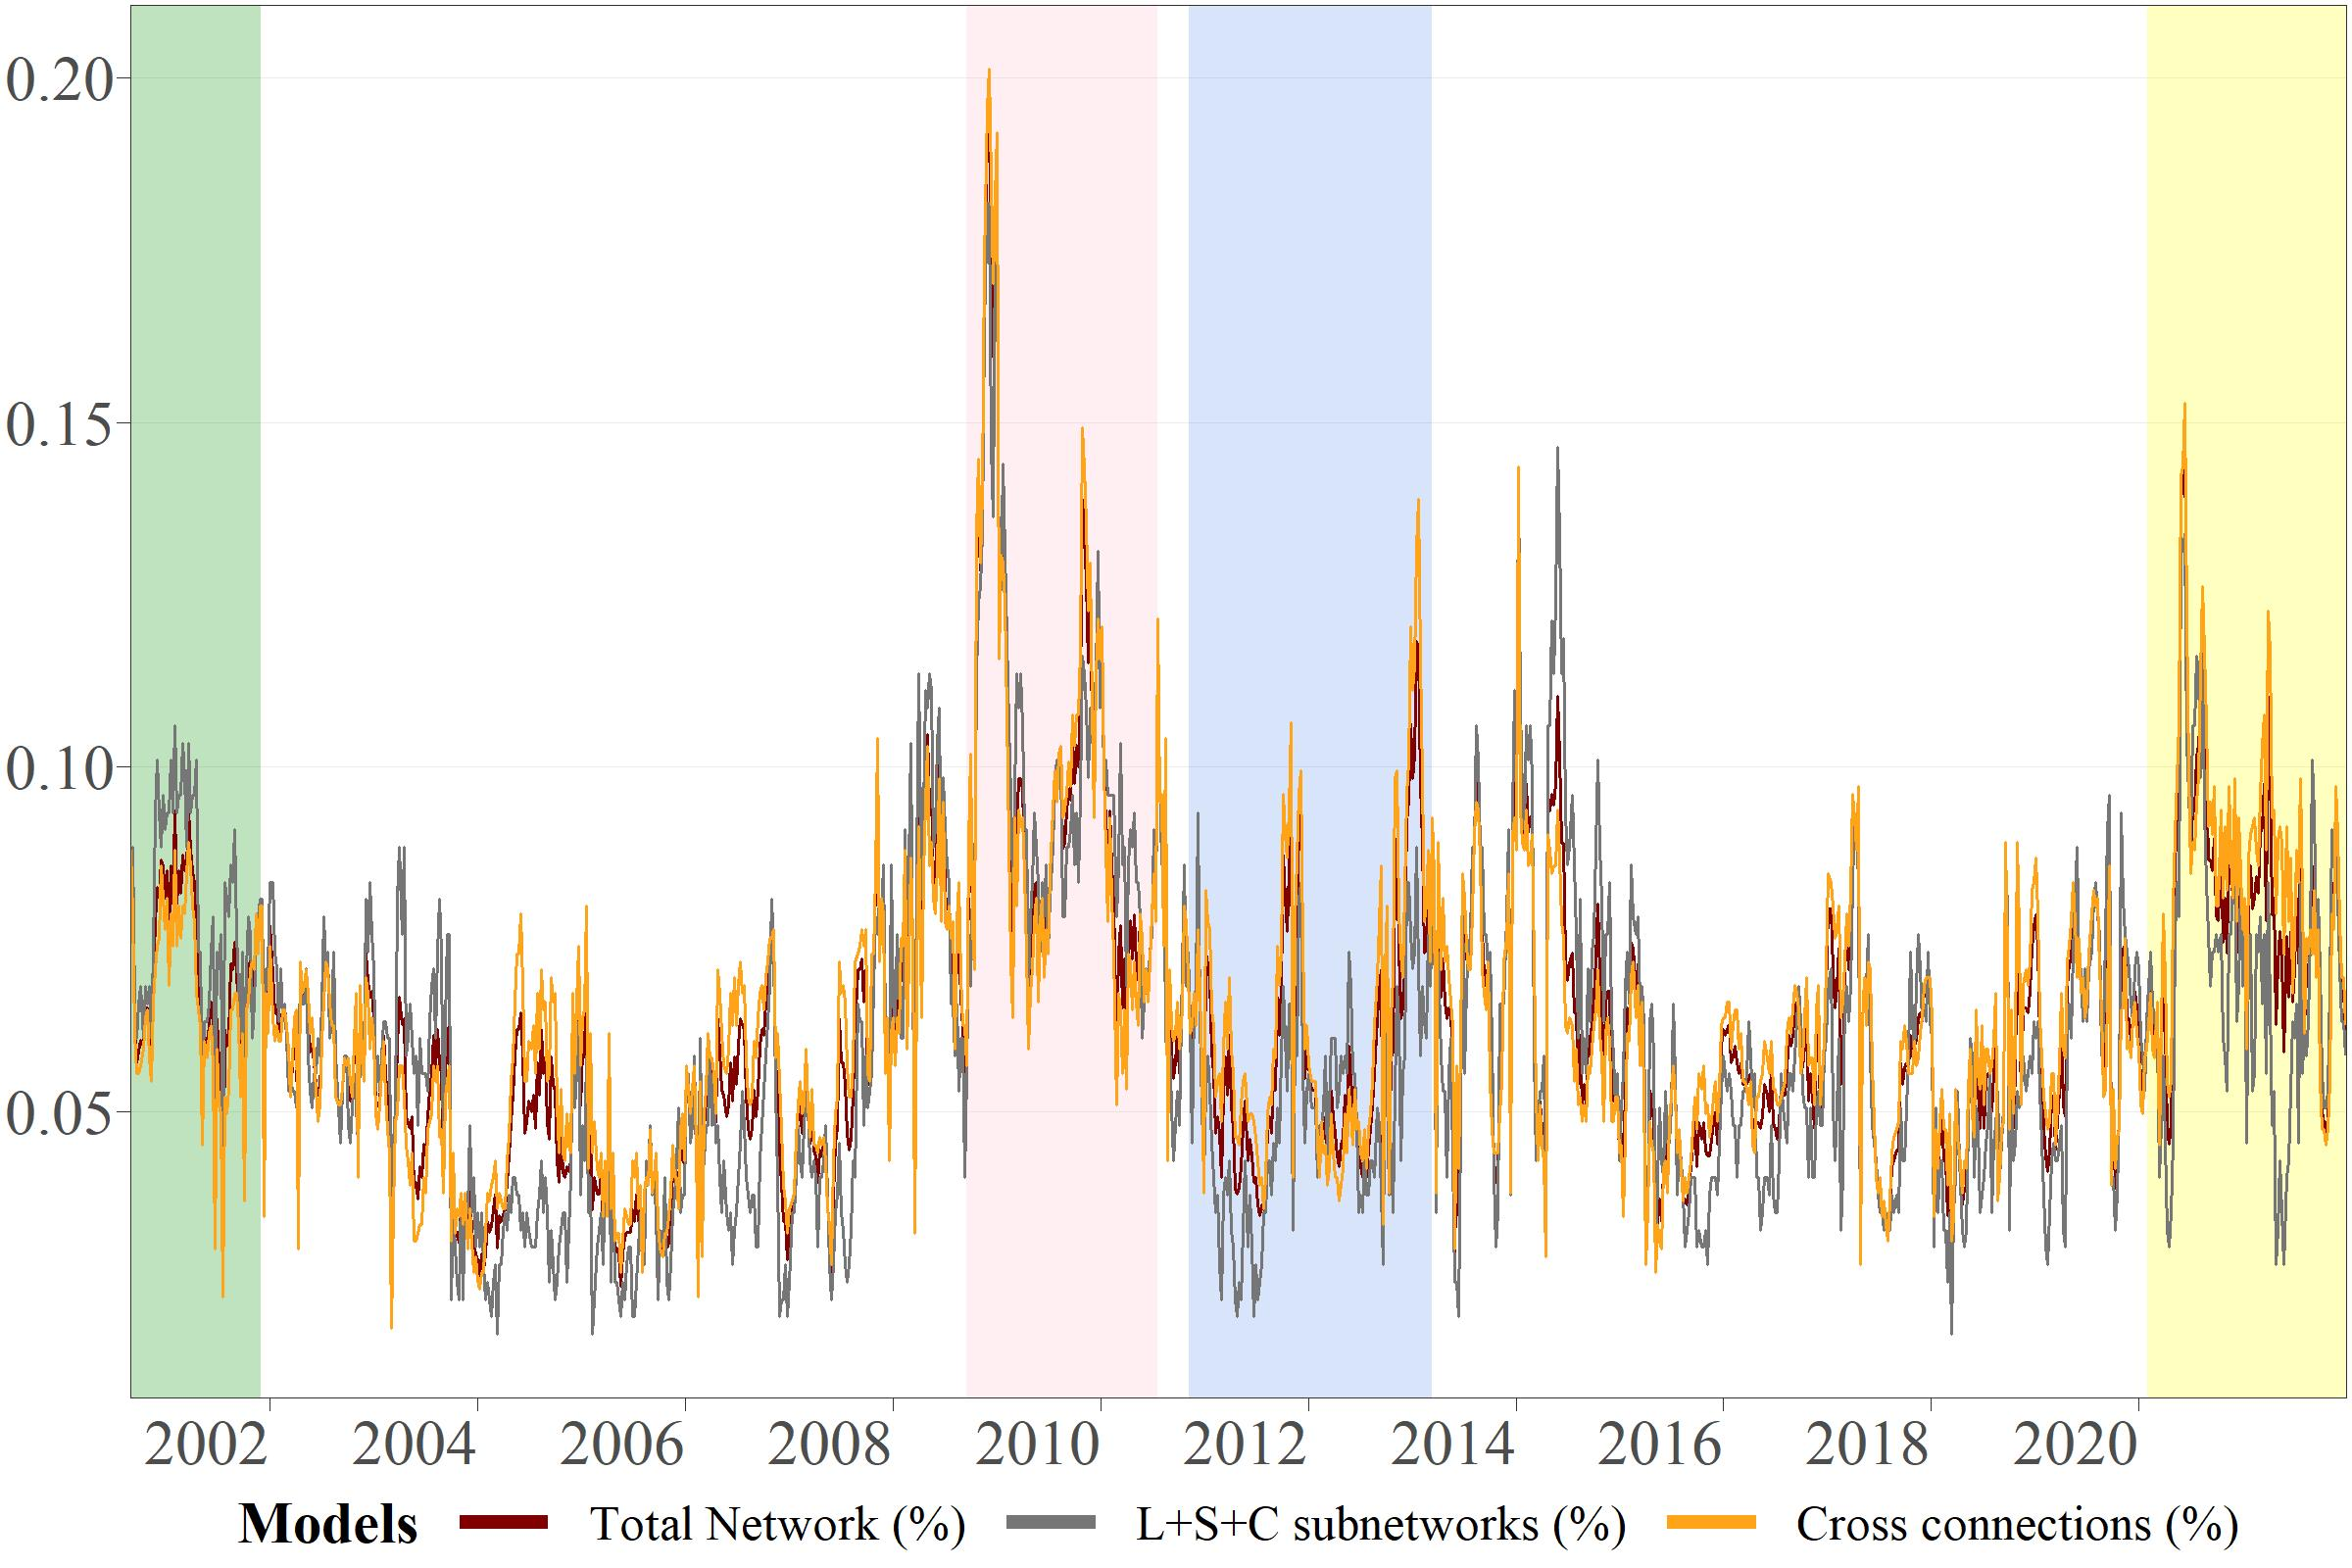
\includegraphics[width=\linewidth]{500edgesDistribution}
    \caption{\textbf{500 observation long rolling window}}
  \end{subfigure}
  \hfill
  \begin{subfigure}[t]{.5\textwidth}
    \centering
    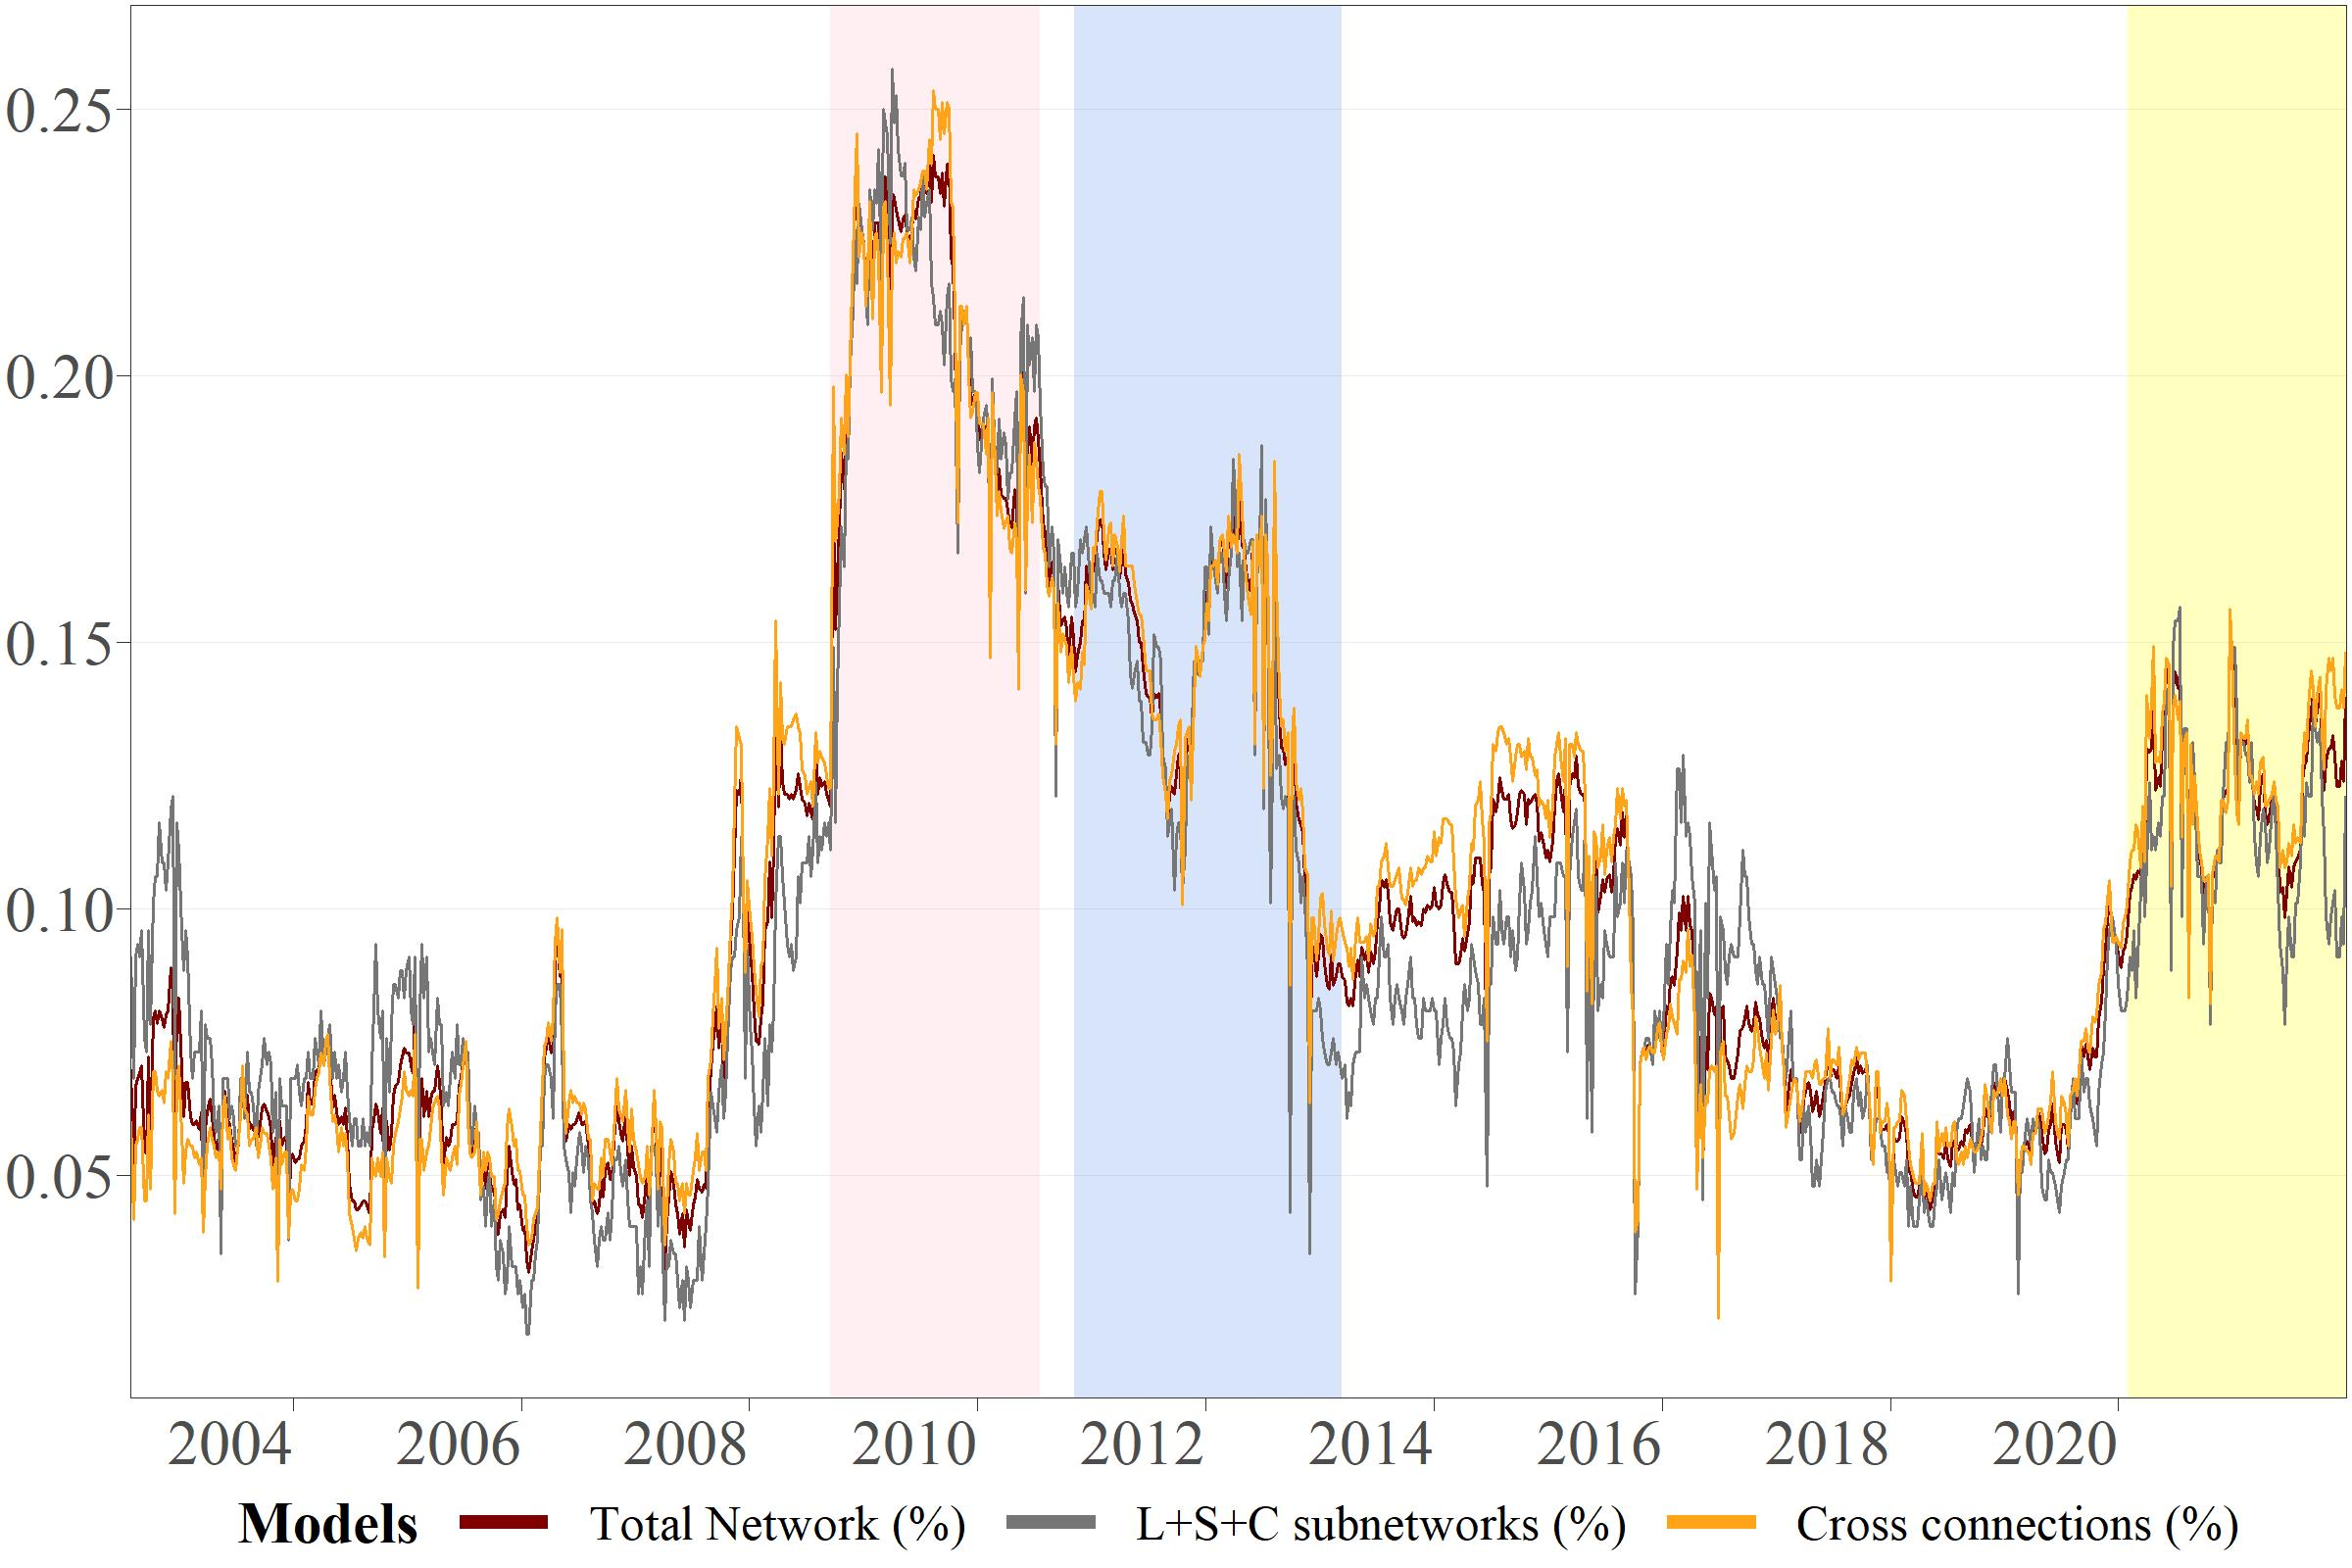
\includegraphics[width=\linewidth]{1000edgesDistribution}
    \caption{\textbf{1000 observation long rolling window}}
  \end{subfigure}
\caption{Summarized edge number by day, resulted by dynamic Toda-Yamamoto analysis}
\label{fig:500and100Longwindowsizes}

\end{figure}














%----------------------------------------------------------------------------------------------------------------------------------------------------

\end{appendices}


\end{document}

